% !TeX program = pdflatex
\PassOptionsToPackage{table}{xcolor}
\documentclass[11pt]{report} 
\usepackage{minted}
\usepackage[utf8]{inputenc}
\usepackage{amssymb}
\usepackage{listings}
\usepackage{xparse}
\usepackage{xspace}
\usepackage{placeins}
\usepackage[english]{babel}
\usepackage{amsmath}
\usepackage{tabularx}
\usepackage{lscape} 
\usepackage{adjustbox}
\usepackage{rotating}	
\usepackage{caption}
\usepackage[T1]{fontenc}
\usepackage{amsfonts}


\usepackage{tocloft}
%\setlength{\cftsecindent}{0em}
%\setlength{\cftsubsecindent}{0em}
%\setlength{\cftsubsubsecindent}{0em}

%\renewcommand{\cftsecfont}{\normalfont\bfseries}% titles in bold
%\renewcommand{\cftsecpagefont}{\normalfont\bfseries}% page numbers in bold
\renewcommand{\cftdotsep}{1}
\renewcommand{\cftsecleader}{\bfseries\cftdotfill{\cftsecdotsep}}% dot leaders in bold

\usepackage{tikz}
\usetikzlibrary{automata, positioning, arrows, matrix}
\tikzset{
	->,
	>=stealth,
	node distance=3cm,
	align=center,
	every state/.style={thick, fill=gray!10},
	initial text=$ $
}
\lstset{
	frameround=fttt,
	language=C,
	numbers=left,basewidth=0.5em,
	breaklines=true,
	basicstyle=\ttfamily\color{blue},
	columns=fixed,
	numberstyle=\color{maroon},
}
	
%\usepackage{geometry}
%\usepackage{natbib}
\usepackage{textcomp}
\usepackage[scaled=.81]{beramono}
\usepackage[sc]{mathpazo} % add possibly `sc` and `osf` options
\usepackage{eulervm}
\usepackage[Lenny]{fncychap}
\usepackage{soul}
\setlength{\headheight}{15pt}
\usepackage[llbracket]{stmaryrd}
%\setcounter{tocdepth}{6}
%\setcounter{secnumdepth}{6}
\usepackage{amsthm}
\usepackage{url}
\usepackage{verbatim}
\usepackage{graphicx}
\usepackage{algorithm}
%\usepackage[noend]{algpseudocode}
%\usepackage{qtree}
%\usepackage{subfig}
%\usepackage{mathpartir}
\usepackage{dirtree}
\setminted{
	fontsize=\footnotesize{},
	linenos,
	tabsize=2,
	breaklines,
	frame=lines,
	samepage=true
}

\newcommand{\code}[1]{\textcolor{blue}{\texttt{#1}}}
\newcommand{\gapwedge}{\ \wedge{}\ }
\newcommand{\ruledef}[4]{
	#1 & \texttt{#3} & $\rightarrow{}$ & \texttt{#4} & #2 \\
}
\captionsetup{width=.9\linewidth}
\newtheorem{assumption}{Assumption}
\usepackage{booktabs}
\usepackage{titlesec}
\usepackage{fancyhdr}
\pagestyle{fancy}
%\usepackage[table]{xcolor}

\titleformat{\section}
{\Large\bfseries\rm}
  {\thesection}{1em}{}
  
\titleformat{\subsection}
{\large\bfseries\rm}
  {\thesubsection}{1em}{}

\captionsetup{width=.9\linewidth}

\interfootnotelinepenalty=10000

\fancyhf{}
\lhead{}
\rhead{\rightmark}
\cfoot{\thepage}

\definecolor{dblue}{rgb}{0.1,0.2,0.6}
\definecolor{dgreen}{rgb}{0.1,0.6,0.2}
\definecolor{dred}{rgb}{0.6,0.1,0.1}
\usepackage[linktocpage=true]{hyperref}
\hypersetup{colorlinks,linkcolor={dblue}, citecolor={dred},urlcolor={dred}}  

\usepackage{epigraph}
\renewcommand{\epigraphsize}{\small}

\setlength{\epigraphwidth}{0.66\textwidth}
\renewcommand{\textflush}{flushright} \renewcommand{\sourceflush}{flushright}
\newcommand{\Imp}{\Longrightarrow}
\newcommand{\All}{\bigwedge}


\title{Formalizing the Semantics of Concurrent Revisions}
\author{Christopher Esterhuyse}
\date{\today}

\begin{document}

\begin{titlepage}
	\centering
	
\includegraphics[width=0.22\textwidth, trim={0 0.15cm 0 0}, clip]{img/vu.png}
%	 \hspace{1.3cm}
%	
\includegraphics[width=0.15\textwidth, trim={0 0.74cm 0 0}, clip]{img/uva.eps}
	\par
%	\vspace{1cm}
	{\scshape\huge Vrije Universiteit Amsterdam \par}
	\vspace{1.5cm}
	{\scshape\LARGE Master's thesis\par \par
	\vspace{0.2cm}
	\small \textit{Submitted in partial fulfillment of the requirements for\\ the degree of Master of Science in\\ Parallel and Distributed Computer Systems.}\par}
	\vspace{1.5cm}
	{\Huge\bfseries \rm \textbf{Generating Safe and Fast\\ Coordination code in\\ Rust with Reo}\par}
	\vspace{1.5cm}
	{\Large\itshape\rm \noindent\textit{Christopher Esterhuyse}\\}
	\vspace{1mm}
	\textit{(ID: 2553295)}
	\vfill
		\rm \noindent \textit{supervisors} \\ \vspace{0.15cm}
	\begin{tabular}{r@{\hskip 0.4in}l}
\rm \hspace{3mm} \textbf{Vrije Universiteit Amsterdam} & \textbf{Centrum Wiskunde \& Informatica} \\ 
dr.\ J.\ \textsc{Endrullis} & prof.\ dr.\ F.\ \textsc{Arbab}
\end{tabular}
\begin{comment}
	\vfill
	\rm supervised by\par
	dr.\ J.C.\ \textsc{Blanchette} (VU), first supervisor \par
	prof. dr.\ W.J.\ \textsc{Fokkink} (VU), second supervisor \par
	ir. R. \textsc{Van Dalen} (ING), daily supervisor
	\end{comment}
	\vfill

\begin{comment} TODO EVENTUALLY
1. check citations going out of margins
2. cite extra sources
3. 
\end{comment}
% TODO!! check for everyone's honorifics

% Bottom of the page
	{\large \today\par}
\end{titlepage}

\abstract{
TODO
}

\include{parts/preface}

\tableofcontents
\listoffigures
%\listoflistings
%\listoftables

\newpage

% worry about the page numbers later. I think it's got something to do with HL

\part{Preliminaries}
\chapter{Introduction}	


Traditional, sequential programming has been changing for decades. Over time, languages acquired more and more tools to manage the level of abstraction, such that programs were of higher quality, and with a lower cost to develop~\cite{shaw1984abstraction}. This trend continues to this day. For example, conventionally imperative languages such as Java and C++ have since added functional features, such as closures, to capitalize on their brevity and lack of side effects. Concurrent programming has undergone a similar process. Various paradigms have emerged to offer their own solutions to managing abstraction. \textit{Coordination languages} attempt to reduce the coupling between the logical coordination of a program from its implementation. Their namesake is their efforts to isolate that which makes concurrency distinct from sequential programming: the coordination of actions into interactions. The means by which this is achieved varies. Linda is a well-known example of a coordination language which abstracts away the implementation of coordination actions. Programs are written in terms of read and write operations over a global namespace of tuple variables. In this manner, coordination actions occupy a higher level of abstraction, and are thus more terse, simple and reusable~\cite{gelernter1985generative}.


Reo is a coordination language developed at the CWI in Amsterdam. As with Linda, Reo augments another general-purpose programming language by allowing a more abstract expression of coordination. Unlike Linda, Reo facilitates the `extraction' of a program's coordination logic to a self-contained \textit{protocol specification}. Reo does away with action-centricism; protocols constrain the ways in which data is permitted to flow through a system of graphical nodes, ie.\ protocols define their permitted interactions~\cite{arbab2005abstract}. The specification is translated by the \textit{Reo compiler} to a the target language. The result is a \textit{protocol object}, a data structure which acts as a coordination medium for the system's actors by distributing a set of \textit{ports} through which they are able to send and receive data. In programming these actors, one is able to rely on the protocol object to coordinate port actions such that the system at large adheres to the protocol specification at runtime. Effectively, programmers are able to act on ports without making any assumptions about the environment beyond.

In this work, we aim to extend the Reo compiler and its related tooling such that it can be integrated into the development pipelines of programs in systems languages such as C, C++ and Rust. Chapter~\ref{sec:imperative_form} details the development of a Rust language target for the Reo compiler, whose outputs are interoperable with these languages. We discuss the various representation changes that a Reo protocol specification must undergo before valid Rust can be emitted.

Reo has intuitive \textit{value-passing} semantics, such that data moving through ports is transferred in its entirety, without interference from the actions of other ports. In the realm of shared memory, this has an undesirable na\"ive implementation which must move the contents of large data types repeatedly. Reo-compiled Java code makes use of an optimization whereby values are kept in place, and their references are moved through ports instead. Currently, Reo-generated Java protocol objects are circumstantially subject to data races as a result of applying this optimization. This violates Reo's semantics; actors cannot be certain that a value acquired through a local port is not being accessed by someone else concurrently. Chapter~\ref{sec:protocol_runtime} explains how our Reo-generated Rust combines the language's systems-level memory management with the explicit protocol descriptions of Reo to perform reference-passing and other optimizations such that Reo's semantics are preserved. Other 
optimizations are also explored. Chapter~\ref{sec:benchmarking} provides an evaluation of our implementation at runtime, comparing it to Reo-generated Java, handcrafted Rust, and breaking down its performance in response to properties of the input Reo specification.

Reo's protocols specify which behaviors systems are and are not permitted to exhibit. At runtime, protocol objects organize actions on their boundary ports into permitted interactions. Actions do not succeed until they are permitted. In this manner, port actions at the wrong time will not cause the program to deviate from the protocol, but may cause a loss of program liveness if the operation blocks for an interaction that never comes. For such cases, Chapter~\ref{sec:api} explores the design of \textit{static governors}, structures which allow the programmer to opt into verifying that local actions will not impede program liveness.


\chapter{Background}
\section{Reo}
\label{sec:reo_background}
Reo is a high-level language for specifying protocols. Here, we explore the motivation behind Reo's development, how the language is used, and (at high level) how it works. 
The Reo language has applicability whenever there is a benefit in being able to formalize a communication protocol. However, this work primarily focuses on Reo's role in automatic generation of glue-code for applications.  

\subsection{Motivation}
\label{sec:reo_motivation}
TODO focus on safety properties

Modern software development involves the construction of large and complex projects. Owing to their scale and the heterogeneity of the tasks required, many people are involved in the development of a program at once, and over its development lifetime. The industry has long-since established paradigms for managing the scale of these projects. One tenet of good software design is \textit{modularity}, which describes a structure that, instead of being designed monolithically, is built out of smaller constituent modules. In addition to isolating modules such that they can be re-used in other projects, this design philosophy allows contributors to concentrate on a subset of all the modules at a time. These ideas are well-established in practice; code re-use and separation-of-concerns have been prevalent for some time.

Reo's utility is not only its ability to facilitate modularity. Reo is designed such that properties of the individual modules are \textit{preserved} when modules are \textit{composed} into larger ones. This preservation marks the difference between \textit{gluing} modules together (and hoping for the best), and \textit{composing} them into something guaranteed to have the intended properties. 

\subsection{Language}
\label{sec:reo_lang}
Reo is a \textit{coordination} language. This describes its focus on the specification of the \textit{interactions} between distinct actors. This is in contrast to the usual \textit{action-centric} model common to languages with their roots in sequential programming, where the programs or specifications describe \textit{actions} of entities, relegating any associated interactions to requiring derivation from the actions. In a nutshell, Reo provides a language for describing the behavior of a \textit{system} of actors by explicitly constraining the behavior of the \textit{connector} which serves as their communication medium. 

(TODO define connector. same as component just maybe structural?)

The Reo language is essentially graphic; each connector defines a relation over named \textit{locations}. Complex connectors are defined as the composition of simpler connectors over its locations. This inherently visual language is also often seen in its textual form, usually in the context of machine parsing. 

The simplest \textit{primitive} connectors cannot be subdivided

by listing a set of constituent connectors. The simplest primitive Reo connectors are \textit{channels}(TODO channel vs primitive). Channels by definition cannot be subdivided into constituent connectors, as they are defined by either (a) the model that provides Reo's semantics, or (b) opaque components defined in some target language such as C or Java. The nodes themselves are the other important aspect of the language. Ultimately, each node corresponds to a (logical) location which may hold up to one datum at a time. Reo is by default \textit{synchronous}, and relationships between locations propagates that synchrony. \textit{Locations} are divided into two classes according to whether 

(TODO)

This motivates the Reo's metaphor of propagation of data and back-propagation of data-constraints, corresponding to its namesake, the Greek word for `flow'. The compositional aspect is meaningful when locations are involved in multiple relationships.

\textit{forwards} (by moving data several `hops' at once) and backwards

In addition to re-using nodes inside a connector, connectors are able to expose these nodes for re-use in the connectors \textit{above them} by exposing the node in the connector's \textit{interface}. These exposed nodes are called \textit{ports}, leaning on the metaphor of the connector \textit{moving} some data in and out of itself.

(data flow corresponds with what happens at runtime, except its SYNCHRONOUS by default. Relate to TDS. Talk about replication and equality checks).

(In the context of applications, components that cannot be composed compile to things managed by different threads. at the boundaries, they communicate with ports. Here, there is a meaningful difference between putter and getter. Include example of how a protocol that uses some port A three times still results in a putter-getter pair)


%\subsection{Typical Channels}
%
%In principle, Reo does not enforce the use of any primitive channels in particular. Users are free to use channels that are best-suited to their use case. In practice, a small set of exceptionally simple channels are favoured in literature and in practice owing to their versatility. As such, this work presumes that these consititute the majority of the channels out of which our protocols are composed. Below, we enumerate this set of channels and their behavior.
%
%\begin{enumerate}
%	\item sync($I_0, O_0$)
%	\item fifo1($I_0, O_0$)
%	\item lossy\_sync($I_0, O_0$)
%	\item exclusive\_router($I_0, O_0, O_1$)
%\end{enumerate}


\subsection{Semantic Models}
\label{sec:semantic_models}
Reo took a number of years to take its present shape. It is recognizable as early as 2001, but was presented as a concept before it was formalized, leaving it as a task for future work~\cite{jongmans2012overview}. Later, This several different approaches to formal semantics were developed. For our purposes, it suffices to concentrate only on the small subset of the semantics to follow. For additional information, the work of Jongmans in particular serves as a good entry point\cite{jongmans2012overview}.


Starting with the fundamentals, a \textbf{stream} specifies the value of a variable from data domain $D$ changing over the course of a sequence of events. Usually streams are considered infinite, and so it is practical to define them as a function $\mathbb{N}\mapsto{}D$. A \textbf{timed data stream} (TDS) takes this notion a step further, annotating each event in the sequence with an increasing \textit{time stamp}. A TDS is defined by some tuple $(\mathbb{N}\mapsto{}\mathbb{R}, \mathbb{N}\mapsto{}D)$, or equivalently, $\mathbb{N}\mapsto{}(\mathbb{R}, D)$ with the added constraints that time must increase toward infinity\cite{arbab2004modeling}. By associating one TDS with each \textit{named variable} of a program, one can represent a \textit{trace} of its execution. TDS events with the same time stamp are considered simultaneous, allowing reasoning about \textit{snapshots} of the program's state over its run time. These traces can be practically visualized as \textbf{trace tables}, with variables for columns and time stamps for rows by representing the absence of data observations using a special `silent' symbol \textbf{*}, referring \textit{silent behavior}. In this work, we use `trace tables' to refer to both the visualization and to a program trace as a set of named TDS's. The runs of finite programs can be simulated either by bounding the tables (constraining the TDS domain to be finite), or by simulating finite behavior as infinite by extending the `end' forevermore with silent behavior. Table~\ref{tab:fifo1_eg} gives an example of a trace table for some program with two named variables.


\begin{table}[]
	\centering
	\begin{tabular}{l|cc}
		$\mathbb{R}$  & A & B \\ \hline
		0.0 & 0 & * \\
		0.1 & * & 0 \\
		0.2 & * & * \\
		0.3 & 1 & * \\
		0.4 & * & 1
	\end{tabular}
	\caption[Trace table of a system adherent to fifo1.]{Trace table comprised of TDS's for variables $A$ and $B$. This trace represents behavior that adheres to the \textit{fifo1} protocol with input and output ports $A$ and $B$ respectively.}
	\label{tab:fifo1_eg}
\end{table}


One of it's earlier \textit{coalegebraic models} represented Reo connectors as \textbf{stream constraints} (SC) over such TDS tables in which variables are ports~\cite{arbab2004reo}. Here, constraints are usually defined in first-order \textit{temporal logic}, which allows the discrimination of streams according to their values both now and arbitrarily far into the future\footnote{Not all variants of temporal logic are equally (succinctly) expressive. It requires a notion of `bounded lookahead' to express a notion such as `$P$ holds for the next 3 states' as something like $\square ^{1-3} P$ rather than the verbose $(\square P \wedge \square \square P \wedge \square \square \square P)$.}. This model is well-suited for translating from the kinds of safety properties that are typically desired in practice. Statements such as `$A$ never receives a message before $B$ has communicated with $C$' have clear mappings to temporal logic, as often it is intuitive to reason about safety by reasoning about future events. Table~\ref{tab:fifo1_eg} above shows the trace of a program that adheres the \textit{fifo1} protocol with ports $A$ and $B$ as input and output respectively.

SC are unwieldy in the context of code generation. In reality, it is easier to predicate one's next actions as a function of the \textit{past} rather than the future. Accordingly, \textbf{constraint automata} (CA) was one of the \textit{operational models} for modeling Reo connectors that has a clearer correspondence to stateful computation. Where an NFA accepts finite strings, a CA accepts trace tables. Thus, each CA represents some protocol. Programs are adherent to the protocol if and only if it always generates only accepted trace tables. From an implementation perspective, CA can be thought to enumerate precisely the actions which are allowed at ports given the correct states, and prohibiting everything else by default. A CA is defined with a state set and initial state as usual, but each transition is given \textit{constraints} that prevent their firing unless satisfied; each transition has both (a) the \textit{synchronization constraint}, the set of ports which perform actions, and (b) a \textit{data constraint} predicate over the values of ports in the firing set at the `current' time step. For example, Listing~\ref{tab:fifo1_eg} above is accepted by the CA of the \textit{fifo1} connector with all ports of binary data type $\{0,1\}$. Observe that here the automaton discriminates the previously-buffered value (`remembering' what $A$ stored) by distinguishing the options with states $q_{f0}$ and $q_{f1}$. As a consequence, it is not possible to represent a \textit{fifo1} protocol for an infinite data domain without requiring infinite states.
\begin{figure}[ht]
	\centering
	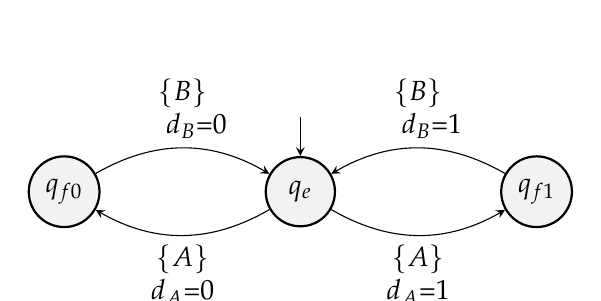
\begin{tikzpicture}
	\node[state, initial above] (q0) {$q_{e}$};
	\node[state, left of=q0] (q1) {$q_{f0}$};
	\node[state, right of=q0] (q2) {$q_{f1}$};
	\draw
	(q0) edge[bend left, below] node{$\{A\}$\\$d_A$=0} (q1)
	(q1) edge[bend left, above] node{$\{B\}$\\\hspace{1em}$d_B$=0} (q0)
	
	(q0) edge[bend right, below] node{$\{A\}$\\$d_A$=1} (q2)
	(q2) edge[bend right, above] node{$\{B\}$\\\hspace{1em}$d_B$=1} (q0)
	;
	\end{tikzpicture}
	\caption[CA for fifo1 connector.]{CA for the \textit{fifo1} protocol with ports $A$ and $B$ sharing data domain $\{0,1\}$.}
	\label{fig:fifo1_ca}
\end{figure}

Later, CA were extended to include \textit{memory cells} (or \textit{memory variables}) which act as value stores whose contents \textit{persist} into the future. Data constraints are provided the ability to assign to their \textit{next} value, typically using syntax from temporal logic (eg: $m'$ is the value of $m$ at the next time stamp). Figure~\ref{fig:fifo1_ca_mem} revisits the \textit{fifo1} protocol from before. With this extension, the task of persistently storing $A$'s value into the buffer can be relegated to $m$, simplifying the state space significantly. This change also makes it possible to represent connectors for arbitrary data domains, finite or otherwise.



\begin{figure}[ht]
	\centering
	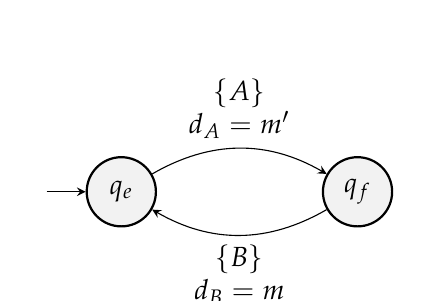
\begin{tikzpicture}
	\node[state, initial] (q0) {$q_{e}$};
	\node[state, right of=q0] (q1) {$q_{f}$};
	\draw
	(q0) edge[bend left, above] node{$\{A\}$\\$d_A=m'$} (q1)
	(q1) edge[bend left, below] node{$\{B\}$\\$d_B=m$} (q0)
	;
	\end{tikzpicture}
	\caption[CA with memory for fifo1 connector.]{CA with memory cell~$m$ for Reo connector~$fifo1$ with arbitrary data domain~$D$ common to ports~$A$ and~$B$. Two states are used to track to enforce alternation between filling and emptying~$m$.}
	\label{fig:fifo1_ca_mem}
\end{figure}


For the purposes of Reo, we are interested in being able to compute the composition of CAs to acquire a model for the compositions of their protocols. Figure~\ref{fig:fifo2_ca} shows an example of such a composition, producing \textit{fifo2} by composing \textit{fifo1} with itself. This new protocol indeed exhibits the desired behavior; the memory cells are able to store up to two elements at a time, and $B$ is guaranteed to consume values in the order that $A$ produced them. Even at this small scale, we see how the composition of such CA have a tendency to result in an \textit{explosion} if state- and transition-space. When seen at larger scales, a \textit{fifo$N$} buffer consists of $2^N$ states. The problem is the inability for a CA to perform any meaningful \textit{abstraction}; here, it manifests as the automaton having to express its transition system in undesired specificity. Intuitively, the contents of $m_0$ are irrelevant when $m_1$ is drained by $B$, but the CA requires two transitions to cover the possible cases in which this action is available. In the context of accepting existing trace tables, data constraints are evaluated predictably. However, in the case of code generation we are able to treat the data constraint instead as a pair of (a) the \textit{guard} which enables the transition as a function of the \textit{present} time stamp, and (b) the \textit{assignment}, which may reason about the next time step, and which we are able to guarantee by \textit{assigning} variables. As such, data constraints are broken up into these parts where possible. Figure~\ref{fig:fifo2_ca} and others to follow formulate their data constraints such that the guard and assignment parts are identifiable wherever it is practical to do so.


\begin{figure}[ht]
	\centering
	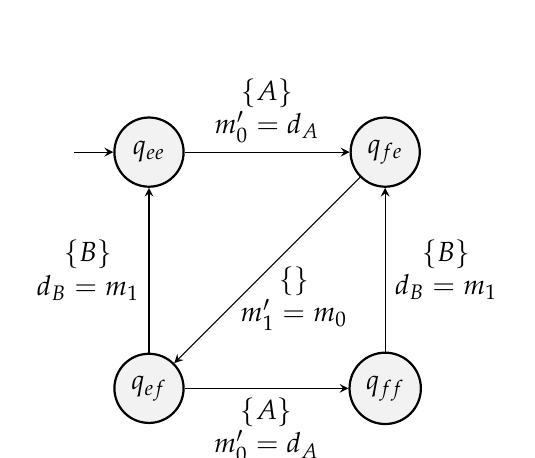
\begin{tikzpicture}
	\node[state, initial]      (qee) {$q_{ee}$};
	\node[state, right of=qee] (qfe) {$q_{fe}$};
	\node[state, below of=qfe] (qff) {$q_{ff}$};
	\node[state, below of=qee] (qef) {$q_{ef}$};
	\draw
	(qee) edge[above] node{$\{A\}$\\$m_0'=d_A$} (qfe)
	(qfe) edge[below] node[pos=0.43]{$\quad{}\{\}$\\$\quad{}m_1'=m_0$} (qef)
	(qff) edge[right] node{$\{B\}$\\$d_B=m_1$} (qfe)
	(qef) edge[below] node{$\{A\}$\\$m_0'=d_A$} (qff)
	(qef) edge[left] node{$\{B\}$\\$d_B=m_1$} (qee)
	;
	\end{tikzpicture}
	\caption[CA with memory for fifo2 connector.]{CA with memory cells $m_0$ and $m_1$ for the \textit{fifo2} connector with an arbitrary data domain for ports $A$ and $B$. Transitions are spread over the state space such that the automaton's structure results in the \textit{first-in-first-out} behavior of the memory cells in series.}
	\label{fig:fifo2_ca}
\end{figure}


\begin{figure}[ht]
	\centering
	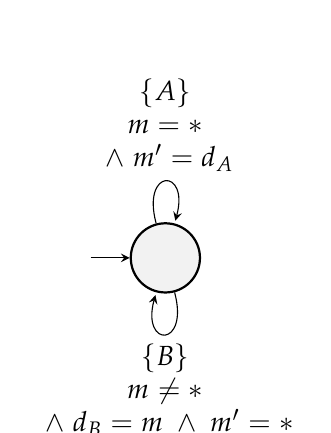
\begin{tikzpicture}
	\node[state, initial] (q0) {$ $};
	\draw
	(q0) edge[loop above] node{$\{A\}$\\$m=*$\\$\gapwedge{}m'=d_A$} (q0)
	(q0) edge[loop below] node{$\{B\}$\\$m\neq{}*$\\$\gapwedge{}d_B=m\gapwedge{}m'=*$} (q0)
	;
	\end{tikzpicture}
	\caption[RBA for fifo1 connector.]{RBA of the \textit{fifo1} connector for an arbitrary data domain common to ports $A$ and $B$. Memory cell $m$ is used both to buffer $A$'s value, and as part of the data constraint on both transitions for \textit{emptying} and \textit{filling} the cell to ensure these interactions are always interleaved. Data constraints are formulated for readability such that the `guard' and `assignment' conjuncts are line-separated.}
	\label{fig:fifo1_rba}
\end{figure}
Evidently, memory cells provide a new means of enforcing how data persists over time. In many cases, it can be seen that the same connectors can be represented differently by moving this responsibility between state- and data-domains. \textbf{Rule-based automata} (RBA) are the cases of CA for which this idea is taken to an extreme by relying only on memory cells entirely; RBAs have only one state. Figure~\ref{fig:fifo1_rba} models the \textit{fifo1} connector once again, this time as an RBA. Aside from the added expressivity, RBAs benefit from being cheaper to compose. As the state space is degenerate, RBAs may be easily re-interpreted into forms more easy to work with. \textbf{Rule-based form} (RBF) embraces the statelessness of an RBA as a single formula, the \textit{disjunction} of its constraints. In this view, Dokter et al.\ defines their composition of connectors such that, instead of exploding, the composed connector has transitions and memory cells that are the \textit{sum} of its constituent connectors\cite{dokter2018rule}.



\begin{figure}[ht]
	\centering
	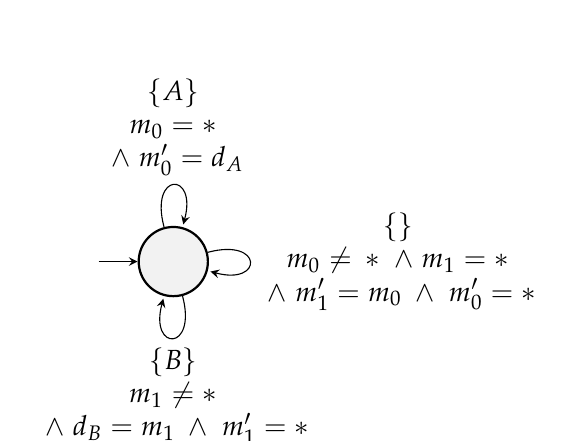
\begin{tikzpicture}
	\node[state, initial] (q0) {$ $};
	\draw
	(q0) edge[loop above] node{$\{A\}$\\$m_0=*$\\$\gapwedge{}m_0'=d_A$} (q0)
	(q0) edge[loop right] node{$\{\}$\\$m_0\neq{}*\gapwedge{}m_1=*$\\$\gapwedge{}m_1'=m_0\gapwedge{}m_0'=*$} (q0)
	(q0) edge[loop below] node{$\{B\}$\\$m_1\neq{}*$\\$\gapwedge{}d_B=m_1\gapwedge{}m_1'=*$} (q0)
	;
	\end{tikzpicture}
	\caption[RBA for fifo2 connector.]{RBA of the \textit{fifo2} connector for an arbitrary data domain common to ports $A$ and $B$. Memory cells $m_0$ and $m_1$ are drained by $B$ in the order they are filled by $A$, and have a capacity of 2 elements. Data constraints are formulated for readability such that the `guard' and `assignment' conjuncts are line-separated.}
	\label{fig:fifo2_rba}
\end{figure}



RBAs have a structure more conducive to \textit{simplification} of the transition space, such that one RBA transition may represent several transitions in a CA. Figure~\ref{fig:fifo2_rba} shows how how this occurs for the \textit{fifo2} connector. Where the CA in Figure~\ref{fig:fifo2_ca} must distinguish the cases where $A$ fills $m_0$ as two separate transitions, the RBA is able to use just one; likewise for the transitions representing cases where $B$ is able to drain $m_1$. This `coalescing' of transitions in RBAs is possible owing to the collapsing of their state space. Even without an intuitive understanding of why such transitions can be collapsed, such cases may often be identified only by inspecting the syntax of the data constraints. For another example of CA, a na{\"i}ve translation to RBA might produce two transitions with data constraints $m=*\wedge{}\;X$ and~$m\neq{}*\wedge{}\;X$ for some~$X$, which are both covered by a single data constraint $X$. As both RBA and RBF share this property, we usually refer to RBA transitions and RBF disjuncts as \textit{rules}, giving these models their name. By distinguishing CA transitions from RBA rules in terminology, we are perhaps more cognizant of the latter's increased ability to \textit{abstract} away needless data constraints. 

\begin{listing}[ht]
	\inputminted[]{java}{putget.java}
	\caption[Type state automaton in Java.]{An example of a program which implements a two-state automaton in the Java programming language. Observe that the behavior of states $A$ and $B$ are encoded implicitly in the \textit{structure} of the program, while determining which of the two in $A$ are available $A$ requires a check ar runtime.}
	\label{listing:putget}
\end{listing}
Typically, Reo has used the $Data$ domains in both CA and RBA as parallels to the data-types of the ports. In most of the languages in which Reo protocols are implemented, the discriminants of such types are not distinguished statically. For example, the C language lacks a way to statically enforce a that function \code{void foo(int x)} is only invoked when $x$ is prime. Instead, checks at runtime are used to specialize behavior. On the other hand, the state-space is simple enough to afford a practical translation into the structure of the program itself, requiring no checking at runtime. For example, Listing~\ref{listing:putget} shows an intuitive representation of a connector that alternates between states $A$ and $B$, getting data $x$ from its environment in $A$, and emitting $x$ when $x=3$. Observe that there is no need to protect operations behind a runtime-check of \textit{which} state the corresponding CA is in. This observation has implications for the behavior of implementations of RBAs, as they `cannot remember' which state they are in and must thus perform more checking. In practice, the overhead of this checking is manageable, and does not \textit{explode} under composition as the state space of CAs tend to do. The representation of automata in programming languages is explored in more detail in Section~\ref{sec:type_state}

\subsection{The Reo Compiler}
TODO ask Sung to summarize the history of the Reo compiler. give a summarized story here. 

The compiler aims to take the low-level implementation of a protocol out of the application developer's hands. Given a protocol specification, the compiler generates the \textit{glue code} and 

TODO focus on RBA

\begin{listing}[ht]
	\inputminted[]{text}{fifo1.rba.treo}
	\caption[Fifo1 connector specfication in textual Reo language.]{TODO.}
	\label{listing:fifo1_treo}
\end{listing}


The steps from Reo specification to the generated glue code can be better understood when broken down into stages:

\begin{enumerate}
	\item \textbf{Specification expansion}\\
	The composed definitions of Reo components are unrolled to the channel-level until the protocol is represented by one large automaton with many nodes.
	
	\item \textbf{Minimization}\\
	Nodes not in the protocol's interface are \textit{hidden} and the RBA is minimized. This step produces a new, simpler automaton with the same behavior and interface.
	
	\item \textbf{TODO PUTTERS AND GETTERS}
	
	\item \textbf{Linking and Code Generation}\\
	The finished source code is generated from the resulting internal-representation. Those associated with functions in the target language are linked accordingly, and the rest are parsed and translated from the operational semantics of Reo to suitable target-language operations (such as data movement and duplication). The rules of the internal state are translated to the runtime definition of a protocol component object. An entrypoint to instantiating this protocol object is generated with the appropriate interface. The specifics of this step vary per target language.
\end{enumerate}

\section{Imperative Languages}
In this section we briefly introduce the properties relevant for discussion associated with imperative programming languages. In our case, these languages are the targets for the Reo compiler. 

\subsection{Affine Type System}
The notion of `affinity' as we use it has its roots in classical and intuitionistic logic. In a type-theoretic proof system, one can attempt to derive some \textit{judgment} $\Gamma\vdash{}t:\tau$ with \textit{statements} assigning \textit{types} to \textit{terms} (here term $t$ is assigned type $\tau$) under context $\Gamma$. A context is simply a list of statements, which can be thought to correspond with \textit{assumptions} or \textit{premises}. The judgment holds if one can construct a proof, starting with the judgment and select and applying rules until no `dangling' judgments remain. For example, simply-typed lambda calculus has a type-derivation rule for abstraction, substitution and application~\cite{nederpelt2014type}. Depending on the type system, \textit{structural rules} may additionally be provided for manipulating (`massaging') the context such that other rules may be applied. For example, \textit{weakening} is a common structural rule that allows one to arbitrarily discard statements from the context. Depending on the proof system, this may be useful or even necessary before other rules can be applied such that the proof can be completed. For example, $weakening$ is required to prove $A, t:\tau\vdash t:\tau$, as $var$ cannot be directly applied; $A$ is in the way. One can imagine that the ability to arbitrary replicate, discard and re-arrange terms effectively describes a type system that treats its context like a set.
\[
\begin{aligned}
(var): \frac{}{t:\tau \vdash t: \tau}
&\quad
(weaken): \frac{\Gamma \vdash \Sigma}{\Gamma, A \vdash \Sigma}
&\quad
(contract): \frac{\Gamma, A, A \vdash \Sigma}{\Gamma, A \vdash \Sigma}
\end{aligned}
\]

\textit{Affine} type systems are characterized by the absence of the \textit{contraction} rule. Proofs cannot replicate statements at will, and thus they are a finite resource in the proof, \textit{consumed} by the application of rules~\cite{walker2005substructural}.

As type systems do in general, type affinity excludes some programs from being expressed. In the context of programming languages, why would we want this? Of course, the hardware has no problem replicating the bytes representing some integer. Why then do we limit ourselves? This argument can be made for type systems in general; the machine likewise has no problem re-interpreting the bytes storing a string as an integer. This limitation is a feature in and of itself as long as the programs lost are usually somehow `undesirable'. For example, it is exceedingly common practice to dedicate a memory region to one type for the duration of the program. The reasons for this are primarily for the programmer and not the program; it is simply easier to distinguish values by type such that values only move between them when explicitly `moving' in memory.


\subsection{The Rust Programming Language}
\label{sec:rust_language}
The Rust programming language is most similar to C++, being a general-purpose, imperative systems-level programming language with C-like syntax. What sets Rust apart is its memory model. Rust is not a memory-managed language, and has no runtime whatsoever. Instead, the language relies on its \textit{ownership system} to predictably insert allocations and deallocations at the right moment such that it \textit{runs} much as C++ would without exposing these details to the programmer. To make this possible, the Rust compiler keeps track of the variable binding which \textit{owns} a value at all times. Owned values are affine, and associating them with new variable bindings invalidates their previous binding. In Rust, this is called \textit{moving}, and doubles (at least conceptually) with the re-location of a value in memory. Listing~\ref{listing:move} illustrates how this appears to a programmer; In \code{main}, the variable \code{x} is moved into the scope of \code{func}. The subsequent access of \code{x} on line 8 is invalid, preventing this program from compiling. Once an owned value goes out of scope, it is no longer accessible, and Rust performs any destruction associated with that type. Along with the RAII (`resource acquisition is initialization') pattern popularized by C++, programmers can rest assured that their resources are created and destroyed on demand, without the need for any bookkeeping at runtime.

\subsubsection{Borrowing}

On their own, movement is incredibly restrictive; there is no apparent way to use any resource without destroying it. To reclaim some vital functionality, Rust has the \textit{borrow system} to facilitate the creation and management of types whose ownership is \textit{dependent} on others. Similar to those in C++, programmers are able to create \textit{references} to values (also called `borrows' in Rust terms). These references are new types, and thus do not represent a transference of ownership to a new binding. Listing~\ref{listing:move2} demonstrates the example from before, but now passing the $x$ by reference into \code{func} such that \code{x} is not invalidated. The Rust compiler's \textit{borrow checker} relies on variable scoping to keep track of these borrows to ensure they do not out-live their referent, as these would manifest at runtime as \textit{dangling pointers}. This relationship between value and reference is referred to in Rust as the reference's \textit{lifetime}. Rust performs this static analysis at a per-function basis. As such, it is necessary for programmers to fully annotate the input and output types of functions, but they can usually be \textit{elided} within function bodies. This has an important consequence; the compiler does cross the boundaries between functions to interpret their relationship. 

For some types there is no practical reason to enforce affinity. This is usually the case for primitives such as integers. For these cases, the language uses the \code{Copy} trait to opt-out of Rust's affine management of these resources. Copy-types behave in ways familiar to C and C++ programmers. Listing~\ref{listing:move} from before would compile just fine if Rust's 4-byte unsigned integer type~\code{u32} was used in place of~\code{Foo}.

C and C++ have no inherent support for preventing data races. The programmer is in full control of their resources. It is all too easy to create data races to C by unintentionally accessing the same resource in parallel precautions. One of the tenets of Rust's design is to use its ownership system to prohibit these data races at compile-time. For this reason, Rust has an orthogonal system for \textit{mutability}. References come in two kinds: mutable and immutable. The distinction is made explicit in syntax with the \code{mut} keyword. Rust relies on a simple observation of the common ingredient for all data races: mutable aliasing; only \textit{changes} to the aliased (one resource accessible by multiple bindings) resource manifest as data races. Rust's approach is thus simply to prohibit mutable aliasing by preventing these conditions from co-existing. Mutable references must be \textit{unique} (prohibiting aliasing) and immutable references do not allow for any operations that would mutate their referent (prohibiting mutability). This is the same thinking behind the \textit{readers-writer} pattern for the eponymous lock: there is no race condition if readers coexist, but if one writer exists, it must have exclusive access. 




\begin{listing}[ht]
	\centering
	\inputminted[]{rust}{move.rs}
	\caption[Example of move semantics in Rust.]{Type \code{Foo} is affine. On line 7, $x$ is moved into function \code{func}, consuming it. Accessing $x$ is invalid, and so line 8 raises an error.}
	\label{listing:move}
\end{listing}

\begin{listing}[ht]
	\centering
	\inputminted[]{rust}{move2.rs}
	\caption[Example of borrowing in Rust.]{\code{Foo} is an affine resource. New references to \code{x} are created and sent into code{func} without changing the ownership of \code{x}. Rust's \textbf{borrow checker} ensures that these borrows do not outlive \code{x}.}
	\label{listing:move2}
\end{listing}

\subsubsection{Traits and Polymorphism}
The primary means of polymorphism in Rust is through generic types with \textit{trait bounds}, also called `type parameters'. Traits are most similar to interfaces in Java, categorizing a group of instantiable types by defining abstract functions for which implementors provide definitions. Unlike Java, Rust traits say nothing about fields and data, thus describing only their behavior. In this manner, Rust traits are somewhat like C's header files, but rather to be defined per implementor type. Elsewhere in the program, functions and structures can make use of \textit{generic} types. These types are arbitrary and thus opaque to any behavior save for those common to all Rust types; for example, any type at all can be \textit{moved} or can be \textit{borrowed} in Rust. To perform more specialized operations on these generic types, they can be \textit{bounded} with traits. This acts as a contract between the generic context and its concrete call-site; the caller promises that the generic type is reified only with a type which implements the specified traits, and thus the generic can be used in accordance with the behavior these traits provide. This is demonstrated in Listing~\ref{listing:traits}. Here, \code{something} is a function which can be invoked with \code{T} chosen to be any type implementing trait \code{T}, such as \code{String}. 

\begin{listing}[ht]
	\centering
	\inputminted[]{rust}{traits.rs}
	\caption[Generic type example in Rust.]{Definition of a function \code{something} generic over some type \code{T}, where \code{T} implements trait \code{PrintsBool}. Types can implement this trait by providing a definition for all the associated functions, in this case, only \code{print\_bool}.}
	\label{listing:traits}
\end{listing}

Above, we see how a function can be defined such that it operates on a generic type. However, the function cannot be used until the type is chosen concretely for a particular instance. This choice is called \textit{dispatch}, and Rust offers two options: static and dynamic. \textit{Static dispatch} (also called `early binding') is used when the called function can be informed which concrete type has been chosen statically, as the caller knows it at the call-site. During compilation, the generic function is \textit{monomorphized} for the type chosen in this manner on a case-by-case basis, generating binary specialized for that type as if there were no generic at all. Static dispatch is used in C++ templates, and opted-out with the keyword \code{virtual}. This is Rust's second option: \textit{dynamic dispatch} (also called virtual functions or late binding) where the generic function exists as only one instance, and all of the specialized operations on the generic type are resolved to concrete functions at runtime by traversing a layer of indirection: functions are \textit{looked up} in a virtual function table (vtable). Java uses such virtualization extensively, which allows a lot of flexibility such as allowing functions to be \textit{overridden} by downstream inheritants. Precisely how a language represents virtual functions and lays out the data in memory varies from language to language. Rust uses the \textit{fat pointer} representation in its \textit{trait objects}. Concretely, some generic object which is known only to implement trait~\code{Trait} is represented as a pair of pointers; the first pointing to the actual object' data, and the second pointing to a dense structure of meta-data and function pointers for the methods of~\code{Trait}, usually embedded into the text section of the binary by the Rust compiler itself.

Rust uses traits for just about everything. Some traits are defined in the standard library, and have a degree of `first class' status by having special meaning when used in combination with the language's syntax. For example,~\code{Not} is a trait that defines a single function,~\code{not}, which is invoked when the type is negated using the usual exclamation syntax, ie.\ \code{!true}. Some traits have no associated functions, instead exist for the purpose of communicating information to the compiler. Seen before,~\code{Copy} is a trait which disables the Rust compiler's checks of a value's affinity. \code{Copy}-types may be passed by value. On the other hand, \code{Drop} associates the \code{drop} function with a type, which the compiler will invoke when it goes out of scope; this is the parallel to the definition of destructors in C++. It is common practice in Rust to rely upon common traits such as these for frequently-occurring cases. For example, it is considered good practice to implement \code{Debug} on your custom traits such that they can be printed using \textit{debug print} syntax (eg.\ \code{print!("{:?}", foo)}) for programmers depending on your work.

\subsubsection{Enums and Error Handling}
As in C, Rust usually relies on \code{struct} for defining its types. Each is defined as the list of its constituent fields. Creation of these structures necessitates building all of their constituents, and all fields exist at once. By contrast, \textit{sum types} have \textit{variants} only one of which may be present at a time. Arguably, the duck-typing of Python and flexible polymorphism of Java do the work of these sum types; a variable can be bound to \textit{anything} and then its `variant' can be reflected at runtime using some explicit operations (\code{ininstance} and \code{instanceof} respectively). C takes the approach fitting the language's philosophy; \code{union} types represent any one of its constituents but the program is at the mercy of the programmer to interact with it as the correct variant as they see fit. Rust's solution is similar to C's unions, but its focus on safety required the use of \textit{tags}. In Rust, an \code{enum} type is defined with a list of variants, only one of which may exist per intance at a time. At runtime, the variant can be descriminated by explicitly \textit{pattern-matching}, inspecting some implicit meta-data field of the enum stores to reflect which of the variants is in use. Like C's unions, each variant can be an arbitrary type (another struct for example), these variants can be of heterogeneous size, and thus are represeted by the largest of their variants \textit{plus} the space for the tag. 

Unlike Java and Python, Rust has no mechanism for \textit{throwables} which override the default control flow, usually for the purposes of ergonomically handling errors. Instead, Rust represents all recoverable errors in the data domain as enums. The standard library defines \code{Option} and \code{Result} enums, which are monadic in that they \textit{wrap} the `useful' data as one of the variants, but represent the possibility for \textit{other} variants also. They differ in that \code{Option::None} carries no data, and thus \code{Option} is generic only over one type, the contents of the \code{Some} variant. \code{Result}, on the other hand, has two generic types, one for its `successful' \code{Result::Ok} variant, and one for its `unsuccessful' \code{Result::Err} variant. Listing~\ref{listing:enums} gives an example of typical error-handling in Rust; here, \code{divide\_by} relies on \code{Result} to propagate the error for the caller to handle. In circumstances where the error is unrecoverable, Rust uses a thread \textit{panic}, which unrolls the control flow (printing debugging information if an environment variable is set). This is somewhat similar to Java's \code{Error}.

\begin{listing}[ht]
	\centering
	\inputminted[]{rust}{enums.rs}
	\caption[TODO.]{Demonstrating the Rust idiom of using a \code{Result} in return position to propagate exceptions to the caller for handling. Here, \code{main} must \code{match} the return value to acquire the result contained within the \code{Result::Ok} variant.}
	\label{listing:enums}
\end{listing}

\subsection{The Type-State Pattern}
\label{sec:type_state}

The \textit{state} or \textit{state machine} pattern refers to the practice of explicitly checking for or distinguishing transitions between and requirements of states in a stateful object\footnote{Usually, we disregard the effects of terminating the program. Equivalently, this pattern only allows one to describe automata in which every `useful' state reaches some final `terminated' state.}. Usually, these states are distinguished in the data domain of one or more types. Even the lowly \code{Option} type can be viewed as a small state machine as soon as some condition statement specializes operations performed with it. Although its uses are ubiquitous in application development in general, this pattern is particularly useful for those for which the added ability to manage complexity is necessary: video games, for example~\cite{nystrom2014game}.

As the name suggests, the \textit{type state} pattern is an instance of the state pattern, characterized by encoding states as types, which usually are distinct from \textit{data} in their significance to a language's compiler or interpreter. A common approach is to instantiate one of the state types at a time. As an example, consider the scenario where a program wants to facilitate alternation between invoking some functions \code{one} and \code{two} which repeatedly mutate some integer $n$. Listing~\ref{listing:typestateeg} gives an example of what this might look like as a \textit{deterministic finite automaton} in the C language. In this rendering, the expression \code{two(one(START)).n} evaluates to the expected result of $(0 + 1) \cdot{} 2 = 2$. Even for this simple example, the encoding of states as types in particular has its benefits; the expression \code{one(two(START))} may appear sensible at first glance, but the compiler is quick to identify the type mismatch on the argument to \code{one}, making clear that the expression does not correspond to a path through the automaton:
\begin{verbatim}
note: expected 'DoTwo' but argument is of type 'DoOne'
\end{verbatim}

The type state pattern can be applied in any typed language, but it is particularly meaningful in languages where the compiler or interpreter \textit{enforces} its intended use. The example above demonstrates some utility, but a language such as C has no fundamental way to prevent the programmer from \textit{re-using} values. 
If the programmer misbehaves, they can retain their previous states when given new ones, and then invoke the transition operations as they please. It's not much of a state machine if all states coexist, is it? This is not always a problem in examples such as the previous. Here, the types prevent the construction of mal-formed \textit{expressions}, and perhaps this is enough. However, we cannot so easily protect a resource from any side effects of \code{one} or \code{two}; imagine the chaos that would result from these functions writing to a persistent file descriptor.
\begin{listing}[ht]
	\inputminted[linenos,tabsize=2,breaklines,frame=lines]{c}{typestate_eg.c}
	\caption[Type state automaton in C with expressions modeling runs.]{An example of the type-state pattern in the C language. The alternating invocation of \code{one} and \code{two} is translated to type-checking the compiler can guarantee. This example guarantees that well-formed \textit{expressions} can be interpreted as valid paths in some corresponding automaton, as the types must match.}
	\label{listing:typestateeg}
\end{listing}

An affine type system overcomes the shortcoming illustrated above. By treating instances of these types as affine \textit{resources}, the programmer cannot retain old states without violating the affinity of the types. The example looks very similar when translated to Rust, but now a case such as that shown in Listing~\ref{listing:typestateeg2} will result in the compiler preventing the retention of the variable of type \code{DoOne}.

\begin{listing}[ht]
	\inputminted[]{rust}{typestate_eg2.rs}
	\caption[Type state automaton in Rust with execution traces as runs.]{A demonstration of how the type-state encoding shown in Listing~\ref{listing:typestateeg} can leverage affine types to ensure that not only expressions, but \textit{a trace through execution} can be interpreted as valid paths through some corresponding automaton. The compiler correctly rejects this example, which corresponds with attempting to take transition \code{two} twice in a row.}
	\label{listing:typestateeg2}
\end{listing}

\subsection{Proof-of-Work Pattern}
\label{sec:proof_of_work}
Section~\ref{sec:type_state} demonstrates how the type-state pattern can be used as a tool to \textit{constrain} actions the compiler will permit the program to do. Indeed, this is a natural parallel to the affinity of the type system, which guarantees that no resource is consumed repeatedly. The counterpart to affine types is \textit{relevant} types, which defines correctness as each resource being consumed \textit{at least once}. Type systems that are both relevant and affine are \textit{linear}, such that all objects are consumed exactly once.

There is no way to create true relevance or linearity in user-space of an arbitrary affine type system; any program which preserves affinity is able to exit at any time without losing affinity. How are we able to enforce a behavior if it is correct to exit at any time? \textit{Proof-of-work} is a special case of the type-state pattern which allows the expression of a relevant type \textit{under the assumption that the program continues its normal flow}; ie. system exits are still permitted. The trick to enforcing the use of some object \code{T} is to specify that a type is a function which must \textit{return} some type \code{R}, and to ensure that \code{R} can \textit{only} be instantiated by consuming \code{T}. Clearly, we cannot prevent \code{T} from being destroyed in some other way, but we are able to prevent \code{R} from being \textit{created} any other way.

Realistic languages have many tools for constraining what users may access. Java has \textit{visibility} to prevent field manipulations. Rust has \textit{orphan rules} to prevent imported traits from being implemented for imported types. Languages without any such features won't be able to prevent users from creating the return type \code{R} without consuming \code{T}. In these cases, another option is \textit{generative types} which, among other things, allow us to further distinguish types with different origins. Here, generative types may be used to ensure not just \textit{any} \code{R} is returned, but a particular \code{R} within our control. As this work uses the Rust language for concrete implementations, we will rely on its ability to prohibit the user from creating \code{R} by using \textit{empty enum types} for types with no data nor type constraints, and by making its fields and constructors \textit{private} otherwise\cite{exotic_sizes}.

Consider the following illustrative scenario: We wish to yield control flow to a user-provided function. Within, the user is allowed to do whatever they wish, but we require them to invoke \code{fulfill}  exactly once (which corresponds to `consuming \code{R}'). How can we express this in terms the compiler will enforce? Listing~\ref{listing:promise} demonstrates a possible implementation (omitting all but the essence of `our' side of the implementation). The user's code would then be permitted to invoke \code{main} with their own choice of callback function pointer. Our means of control is the interplay between dictating both (a)
the \textit{signature} of the callback function and (b) prohibiting the user from constructing or replicating \code{Promise} or \code{Fulfill} objects in their own code.

\begin{listing}[ht]
	\inputminted[]{rust}{promise.rs}
	\caption[Proof of work pattern example of `promises'.]{A demonstration of proof-of-work pattern. Here, the user is able to execute \code{main} with any function as argument, but it must certainly invoke \code{fulfill} exactly once.}
	\label{listing:promise}
\end{listing}


\part{Contributions}
\chapter{Code Generation}
\label{sec:imperative_form}







\section{Two-Phase Code Generation}
In this section, we explain and motivate our approach of segmenting the code generation process into two distinct phases. Throughout, we refer to the precedent set by the existing Reo compiler backend for generating code in the Java language, as it has seen the language most similar to Rust which has seen significant development.   

\subsection{Generation Sub-tasks}
Reo specifications represent connectors declaratively as relations between ports. They are thus well-suited to reasoning about the protocol's properties. In contrast, our target imperative languages such as Java and Rust represent computation such that it corresponds more closely to machine instructions; they are imperative, laying out sequences of actions which together emerge as interaction at runtime. Where interactions in the former can be oriented around the synchronous observations of port values, interactions of the latter must be expressed as sequences of actions, laid out over time. Implementing algorithms for translating between these forms must take care that the translation procedure between these forms preserves the semantics as intended; choosing the incorrect ordering can change the nature of the emergent interaction in unexpected ways. For example, reading memory cell \textit{before} writing it corresponds to a different interaction than reading it \textit{after} writing it. 

Rust and Java have in common their strongly-typed language, while  is untyped. To facilitate the desired level of specificity for connectors, the \textit{textual Reo} language has support for optional \textit{data type annotations} on ports, which are retained by the Reo compiler for use by the relevant backend. How these annotations are used is not specified, as their interpretation is only sensible for target languages in a case-by-case basis. To us, these annotations are understood as types which the associated ports must be capable of transmitting. For our typed languages, typing information must be injected such that the emitted target code is valid.

Regardless of the intermediate representation, protocol objects must ultimately be emitted in the target language. Aside from expression in the correct syntax, the end result must make explicit any work required to make it \textit{executable} with the desired runtime behavior. Even simple concepts require the support of auxiliary book-keeping structures to maintain the protocol object's state, and specialized \textit{concurrency primitives} are needed to ensure that actions compose into interactions at runtime in the expected way. Clearly, this is very particular to the target language, as they vary greatly on how they fundamentally express operations on data at a granular level.

In summary, we identify and name three sub-tasks of generating target language protcol objects from a Reo protocol description:
\begin{itemize}
	\item [$T_{act}$] Synchronous interactions must be decomposed into asynchronous actions, with the roles of each participant laid out in a sequence.
	\item [$T_{type}$] Ports must be given data types such that they agree with any (optional) type-annotations in the Reo specification, and successfully type-check in the target language.
	\item [$T_{run}$] Details necessary to make the result runnable are included. Symbolic actions are represented as concrete operations on data.
\end{itemize}


\subsection{Decoupling the Reo Compiler from Rust}
\label{sec:decoupling_reo_rust}
The Reo compiler has an existing backend for generating Java code. It works by generating Java according to the structure of a \textit{template generator}. In this manner, it can be thought of as performing all code-generation sub-tasks at the same time directly from the compiler's intermediate representation. However, the extent to which the Reo compiler is \textit{coupled} to the Java language is reduced through the reliance on a Java library for the granular implementations of structures that are common to all protocol objects; rather than generating these classes each time, the Reo compiler simply generates a dependency. For example, the library defines a \code{Component} interface, for which the code generator produces a protocol-specific implementor class. Consequently, a significant part of $T_{run}$ is delegated to this library.

For $T_{type}$, help comes from the Reo compiler itself, which in its current form was developed with support for Java in mind. This can be seen in the structure of its internal representation. For example, types are given a \textit{default} type in the event the input specification omits a type-annotation; this is no trouble for Java, which can up-cast all classes to~\code{Object} without losing the capabilities on which the protocol relies at runtime, namely (1) equality checks, and (2) object replication\footnote{In the chapter to follow, we discuss the consequence of this approach, as it necessarily assumes that operations for checking equality and replication can be resolved for any types.}.

Only $T_{act}$ is performed almost entirely by the template generator. For simple protocols, this task is relatively easy, as there is not much to add when actions are largely concurrent. For example, replicating the contents of a memory cell into a set of others is simply-done in Java by first reading an object reference, and then overwriting the others one at a time. However, ordering dependencies must be resolved very carefully in the general case. The current Java code generator is susceptible to erroneously observing value $x$ at memory cell $M$ in the event that the observation is synchronous with $M$'s value being overwritten by $x$. Even with the help of the template generator, this translation is sufficiently complex to make detection of these bugs difficult.

Rust is able to mimic Java's approach to create a similar backend through the explicit use of \textit{dynamic dispatch}, such that types can be collapsed to something analogous to Java's \code{Object} class. If done na\"ively, the resulting backend would inherit the problems of its predecessor, and new ones to boot; the Java-like approach is not idiomatic in the context of Rust; it would not make good use of the extensive control of systems resources unique to a systems language. Chapter~\ref{sec:protocol_runtime} to follow goes into detail about the properties of the protocol runtime. Here, it suffices to say that we wish to implement a runtime that does not rely on heap-allocation of its port-values, and thus cannot rely entirely on dynamic dispatch. Furthermore, our runtime wishes to perform more extensive optimizations, relying on the unique abilities of our systems language to manipulate its resources at a low level. All these extensions pose a problem in particular for $T_{run}$, as runtime properties directly influence how the executable protocol objects are represented. Our work in unremarkable in its solution to this problem: we delegate~$T_{act}$ to a Rust library. However, we make this separation more extreme. In a nutshell, we wish to partition the work of code generation into two clear \textit{phases}, the former of which performs tasks~$T_{seq}$ and~$T_{type}$, and the latter of which performs $T_{act}$. To minimize coupling between the modules performing these tasks, the interface between phases is made terse, unambiguous and explicit in the definition of a new intermediate representation of protocol connectors: the \textit{imperative form}.

\subsection{Temporary Simplifications}
Our intention is to isolate the Reo backend from Rust's specifics as extensively as possible. In this manner, we decouple the modules responsible for the code-generation subtasks in accordance with good software engineering practices. Furthermore, it facilitates the \textit{re-use} of the first phase of the code generation process for \textit{other} imperative programming language targets. The section to follow defines imperative form to be as target-language agnostic as possible. However, for the sake of minimizing the disturbance to the Reo tooling ecosystem, we still embrace the per-target structure for Reo code generation for now. As such, the Reo compiler still specifies a Rust language target, and emits executable Rust source as a result. Our representation of the \textit{imperative form} is expressed in Rust syntax (as the \code{ProtoDef} type) such that this reliance on an intermediate representation is invisible to the end user. As far as they are concerned, Reo generates native Rust that just happens to \textit{somehow} make minimal use of Rust-specific syntax. \code{ProtoDef} corresponds closely to the definition of imperative form, facilitating this decision being overturned in future with minimal effort.


\section{Imperative Form}
In this section, we define our new intermediate representation of Reo protocol specifications. We include an intuitive look at how it captures the details of the Reo compiler's internal representation, but such that only $T_{act}$ remains to be performed before the finished Rust source code can be emitted.


\subsection{Intuition}
Imperative form makes explicit the \textit{ordering} of events for which the ordering cannot be arbitrary. In other words, synchronous concurrency can still be expressed, but operations whose correctness relies on it are ordered explicitly. For very simple protocols, imperative form is very similar to the compiler's RBA-like internal representation; they have in common that they partition rules into (1) \textit{guards} which contain the \textit{synchronization-} and \textit{data-constraints}, and (2) \textit{assignments} which mutate the protocl's state and produce observable events such as boundary ports putting and getting. 

Imperative form differs from that of the compiler's intermediate representation the more extensively the protocol makes use of synchronous manipulations of its state, ie.\ the more the protocol's state is mutated \textit{within} a single rule. For example, consider a protocol in RBF with data constraint $f(P_0)=f(P_1)$ and synchronization constraint $\{P_0, P_1\}$ with input (putter) ports $P_{0-1}$. This rule can be understood as ``$P_{0-1}$ fire \textit{if} the results of function~$f$ on their put-values are equivalent''. Here, the results of $f$ clearly cannot be compared until \textit{after} they are computed, but these intermediate values must be \textit{stored} somewhere in the meantime. How can we correctly store these values (mutating the state) \textit{before} we know whether this rule will fire and should thus mutate the state? Our solution is to ensure that these sorts of situations can occur only if these `transient' state-mutations can be \textit{undone} without observable effects; erroneous state mutation is not a problem if it is immediately reverted. Thus, imperative form models a synchronous rule firing as a \textit{transaction} by partitioning its actions on either side of some \textit{commit}-instant. Actions thus then fall into one of two categories:
\begin{itemize}
	\item \textbf{Transient Actions}\\
	Actions \textit{before} committing may only perform mutations of the protocol state that can be \textit{rolled back} reversing their effects. Implicitly, this prohibits any actions that are visible to an outside observer. Actions are also allowed to trigger a rollback and abort.
	
	\item \textbf{Persistent Actions}\\
	Action \textit{after} committing may irrevocably mutate the state and produce observable effects, but may not trigger a rollback.
\end{itemize}

For our example RBF, the check for equality acts as a \textit{guard}, but its computation involves the values put by $P_{0-1}$. To be valid, $f$ is required to be a pure function which cannot be observed to \textit{consume} the values of $P_{0-1}$ (eg.\ by reading them via immutable reference), and is invoked to produce three temporary variables, which can subsequently be checked for equality. If the check fails, all actions \textit{roll back}, discarding our temporary variables and aborting the rule firing. This corresponds to a guard that was not \textit{satisfied}. On the other hand, if the equality passes, the rule \textit{commits} and the values of $P_{0-1}$ are irrevocably consumed (and in this case, discarded). In this way, $P_{0-1}$ only observe their data being consumed if the rule fires.

Conceptualizing an imperative form rule purely as action-sequences gives good intuition for the intention behind the representation. However, this would require concurrent events to be sequentialized. However, many actions are not given in the compiler's internal representation in this form. For example, the ordering of assignments is left unspecified. There is no harm in sequentializing these actions if the end result is indeed sequential. For example, the Java protocol object indeed assigns to memory cells sequentially. Rather than assuming this will always be the case\footnote{Indeed, our final implementation dispatches data movements sequentially, but they are completed concurrently. See Section~\ref{sec:data_exchange}.}, we represents persistent actions as \textit{concurrent} movements from sources to destinations. In the same manner, is it unnecessary to sequentialize the observations in the \textit{guard}; it does not matter the order in which ports are checked for availability. For this reason, imperative form is ultimately represented with three distinct structures (1) unordered transient actions performed before (2) ordered transient actions with rollback, and finally (3) unordered persistent actions.


\section{Definition}
\label{sec:imperative_form_definition}
A protocol description in imperative form must be provided by a single structure which provides mappings for symbolic names such that they can be resolved as they are encountered when traversing the rest of the definition. This \textit{name definition} structure is similar to a \textit{symbol table}. The behavior of the connector itself is defined by a set\footnote{In our implementation, these rules are provided in an ordered list, primarily for the purpose of making for more comprehensible error messages.} of \textit{imperative rules}, each corresponding to an RBA rule, given by a tuple $(P, I, M)$ with:
\begin{enumerate}
	\item \textbf{Premise $P$}\\
	A tuple of three \textit{identifier} sets $(P_R, P_F, P_E)$. Set $P_R$ contains the \textit{synchronization constraint} identical to that of RBAs, referring to the set of ports that `fire'. In the context of a premise, this set describes which ports must be \textit{ready}. $P_F$ and $P_E$ are the sets of \textit{memory variables} which must be known to be full and empty respectively. By definition, any pair of these sets must have an empty intersection. The rule can certainly not consider firing unless all ports are ready and all memory cells are in the specified states. Omitting a port or memory cell represents \textit{undefined state}, and thus is not considered an accessible resource.
	
	\item \textbf{Instructions $I$}\\
	A list of reversible \textit{instructions} which are performed in sequence. These instructions can manipulate resources. As they are tentative, it is also possible to trigger a rollback. Concretely, each instruction is one of:
	\begin{itemize}
		\item $check(p)$\\
		Trigger a rollback if predicate $p$ over data is satisfied.
		\item $fill_P(m, p)$\\Fill an empty memory variable $m$ with the result of a predicate $p$ over available data. It's data type is implicitly \textit{boolean}.
		\item $fill_F(m, f, a)$\\
		Fill an empty memory variable $m$ with the result of invoking function $f$ with parameters $a$, a list of references to data variables with length matching the arity of $f$. It is incorrect for $f$ to \textit{mutate} its arguments, as this would result in observable effects which cannot be rolled back.
		\item $swap(m_0,m_1)$\\
		Swap\footnote{In principle, any reversible data-agnostic manipulation is possible, but swapping values is sufficiently expressive and intuitive for our purposes.} the values in two memory variables~$m_0$ and~$m_1$.
	\end{itemize}
	If a rollback is triggered by $check$, any swapped memory cells are swapped back, and any memory cells whose values were created by $fill_P$ or $fill_F$ are destroyed.
	
	\item \textbf{Movements $M$}\\
	A mapping from \textit{resources} to any identifiers that can act as getters (getter ports and empty memory cells). This represents the \textit{observable effects} of the rule firing after instructions are performed without triggering rollback. 
\end{enumerate}

As an example to demonstrate this representation, the RBA rule in the previous section with data constraint $f(P_0)=f(P_1)$
and synchronization constraint $\{P_0, P_1\}$ can be represented in the imperative-form rule with:
\begin{enumerate}
	\item [$P$] $(\{P_0, P_1\}, \{\}, \{t_0,t_1\})$
	\item [$I$] $[fill_F(t_0, f, [P_0]), \quad{} fill_F(t_1, f, [P_1]), \quad check(t_0 = t_1)]$
	\item [$M$] $\{\}$.
\end{enumerate}

For our purposes, omitting a source identifier $s$ from~$M$ can be interpreted as $s\rightarrow{}\{\}$ by default, understood to mean `discard $s$'. For other applications, it may be preferable to require that each source have an explicitly-defined destination set. For example, this would be useful in the context of a \textit{linear type system} in which data cannot trivially be \textit{destroyed}. 



\section{Code Generation Pipeline}
In this section we explore the translation procedure of protocols, starting from their declarative Reo specification in the Reo compiler's internal representation to executable Rust. This is done in two distinct phases, as explained in Section~\ref{sec:decoupling_reo_rust}. Section~\ref{sec:translation_phase_1} performs translation sub-tasks $T_{act}$ and $T_{type}$, and Section~\ref{sec:translation_phase_2} performs the final sub-task: $T_{run}$.

\subsection{Phase 1: Reo Compiler Backend}
\label{sec:translation_phase_1}
The Rust backend of the Reo compiler translates from the compiler's intermediate representation to Rust. Section~\ref{sec:decoupling_reo_rust} explains how this task is partitioned such that the compiler itself only performs the first of the two phases that comprise this process. Rust is still the target, but rather than generating the protocol object to be executed directly, Reo outputs a source file that contains a \code{ProtoDef}, the Rust-syntax version of a protocol in \textit{imperative form}. 


\subsubsection{Action Sequencing}
The most obvious role the backend plays in the translation process is to spread the contents of the relational, interaction-oriented internal representation over the imperative, action-oriented \textit{imperative rules}. The process begins given (1) the set of port putters in the synchronization set, (2) a mapping from port-getter to \code{Term}, (3) a mapping from port-putter to \code{Term}, and (4) a \code{Formula}, representing the rule's guard. Terms and formulas are recursive data structures, and can both be thought of as \textit{sum types}. The former describes a an expression to be computed at runtime. For example, \code{MemoryCell(A)} and~\code{True} are both terms that can be assigned to memory cells and retrieved by getter-ports. \code{Formula} is similar, but used in the context of predicates; formulas are essentially terms known to have a boolean data-type, and thus come with variants for the usual boolean operations. For example, \code{True}, \code{And(Eq(A,B), Eq(B,C))} are examples of formulas. The backend traverses the compiler's internal representation, constructing imperative form rules one at a time, also populating the associated \code{NameDef} symbol table. For each such rule, it helps to consider each of its distinct structures in isolation, initially without any optimizations:

\begin{enumerate}
	\item [$P$] \textbf{Premise}\\

The first task of the backend is to build the imperative rule's \textit{premise}. Observe that the this step is nearly trivial, as the synchronization set, set of port-getters, and set of port-putters are already provided. The only exception is for memory cells which are \textit{read}, which must be derived by encountering their occurrences inside terms and formulas for the guard and assignments. Clearly, no information is added by explicitly isolating the set of readable memory cells; we are able to derive it despite being absent in the internal representation, and the term is only meaningful if one cannot read from a memory cell \textit{unless} it is marked as readable. We nevertheless perform this preprocessing as it makes explicit that the memory cell must be available for the interaction without having to `look ahead' into terms and formulas. Furthermore, its inclusion provides us a simplifying property: if an identifier does not occur in the premise, it must refer to a \textit{temporary variable}.

\item [$I$] \textbf{Instructions}\\
Next, the backend generates a list of \textit{instructions}, representing the \textit{tentative actions} that may be rolled back if the rule aborts instead of committing. Here, $fill_P$ and $fill_F$ instructions are inserted to compute the results of any evaluations of predicates or functions and bind them to temporary variables. Next, special cases of each memory cell~$M$ synchronously read-from and written-to are detected. For each, a temporary variable $T_M$ is created, and an instruction $swap(M, T_M)$ is appended to~$I$. As a result, data movements can be conducted in parallel without fear of a race condition emerging; although $M$ is logically involved both in reading and writing, these actions are distinguished by name; $M$ is as independent from $T_M$ as any two distinct memory cells. $M$ receives and stores its new (written) value $M$, and its old value can concurrently be read from $T_M$ without interference. Finally, a \textit{check} instruction is appended to the list, parameterized with an analog to the compiler's \code{Formula} type. 

\item [$M$] \textbf{Movements}\\
All port-getters and memory cells which are \textit{written to} are grouped by source to produce~$M$, a mapping from sources to destination sets. Each mapping is additionally annotated with a flag to indicate whether the value is retained at the source, ie.\ the mapping is of type $Identifier \Mapsto{} (boolean, \{Identifier\})$. As an example, moving a value from~$A$ to~$B$ results in $A$ mapping to $(\text{\textit{false}}, \{B\})$.

\end{enumerate}
Clearly, many opportunities exist for optimization of the imperative form, as it affords some degree of \textit{over}-specification and can represent the same specification in different ways. As an example, it is possible to fragment our guard into several \textit{check} instructions. This can be thought of as an explicit encoding of \textit{short-circuiting} behavior. As long as no guard reasons about a temporary variable \textit{prior} to its definition, this is valid. These opportunities were not explored extensively in this work, as instructions in practice tend to be simple enough not to afford many such opportunities. More significant is the \textit{omission} of trivial checks entirely. 

\subsubsection{Type Classification and Constraint}
1. does actions and types, but not symbols
\subsubsection{Code Generation}
wraps it in a function. handles memory initialization

\subsection{Phase 2: Rust Library}
\label{sec:translation_phase_2}

\subsubsection{Soundness Check}

\subsubsection{Data Layout Optimization}
\subsubsection{Meta-State Initialization}
\chapter{Protocol Runtime}
\label{sec:protocol_runtime}
In this section we explore the Rust implementation of Reo-generated protocol objects. Rather that generating the needed structures and behaviour from scratch each time, the Rust back-end follows the precedent of the well-established Java back-end and relies on a single, re-usable dependency for the work common to all protocols. Here, we explore the implementation of this \textbf{Reo-rs} library, picking up where we left off from the generation step in Chapter~\ref{sec:imperative_form} above.

\section{Examining the Java Implementation}
\label{sec:java_examined}
The work of this project can draw from the efforts of previous work on the Reo Compiler. The Java implementation in particular has seen the most frequent and recent updates. This section treats the Java code generator as a touchstone for Reo-generated application code in general. We give a brief overview of the properties inherent to the generated code, and consider the effects of projecting the underlying ideas to the Rust language.

\subsection{Architecture}
Fundamentally, the generated code adheres closely to Reo's literature, revolving around the interplay between \code{Port} and \code{Component} objects. From the perspective of a developer looking to integrate a generated Java protocol into their application, the entry point is the \code{Protocol} component (where `Protocol' is the name of the associated Reo connector).

Running a system requires an initialization procedure: (1) a \code{Port} is instantiated per logical port, (2) a \code{Component} is instantiated per logical component, and (3) pairs of components are linked by overwriting a port-field for both objects with the same instance of \code{Port}. To get things going, each component must be provided a thread to enter it's main loop; in idiomatic Java, this manifests as calling \code{new Thread(C).start()} for each component \code{C}. A simplified example of the initialization procedure is shown in Listing~\ref{listing:java_gen_1} for the simple `sync' protocol which acts as a one-way channel. In this example, the ports are of type \code{String}.


\begin{listing}[ht]
	\centering
	\inputminted[]{java}{java_gen_1.java}
	\caption[Reo-generated Java protocol initialization.]{A simplified example of initialization for a system centered around a \code{Sync} protocol object, which acts as a channel for transmitting objects of type \code{String}. Both ports and components are constructed before they are `linked' in both directions: each port stores a reference to its components, and each component stores references to its ports. The system begins to \textit{run} when each component is given a thread and started.}
	\label{listing:java_gen_1}
\end{listing}


In a sense, this implementation primarily hinges on \code{Port} as a communication primitive between threads, and equivalently, between components. For matters of concurrency, operations on port-data involves entering a \textit{critical region}. In contrast, \code{Components} are used only to store their ports and to be used as name spaces for their \code{run} function which implements their behavior (which corresponds to RBA rules in the case of the protocol component). Essentially, anything that interacts with \code{Port} objects can reify a logical component, whether or not this is done by an object implementing the \code{Component} interface.

\subsection{Behavior}
The representation of protocol rules is very intuitive; a rule is implemented as a block of code which operates on a component's ports. Once generated into Java, the only obvious sign that a component was generated from Reo is its linkage to multiple other components\footnote{The distinction between `protocol' and `compute' components is tenuous at the best of times. If compute components are allowed to interact directly with one another, the distinction observed here disappears also.}. The (simplified) generated \code{Component} code of the `sync' protocol from the previous section is shown in Listing~\ref{listing:java_gen_2}. This demonstrates that rules are indeed \textit{commandified}, in that their behavior is encoded in discernible structures (appropriately called \code{Command}).

The behavior and structure of a component go together, and are generated by Reo at a relatively granular level. As such, the encoding of memory cells is natural also. Memory cells can be found next to ports in the fields of a \code{Component}.

\begin{listing}[h!]
	\centering
	\inputminted{java}{java_gen_2.java}
	\caption[Reo-generated Java protocol class of the sync connector.]{A simplified example of a Reo-generated Java protocol class for the \textit{sync} connector. By convention, it is started by invoking \code{start}, which is a method inherited from the \code{Runnable} interface which \code{Component} extends. This method assumes that all ports are correctly initialized and linked to another `compute' port. Its RBA-like behavior comes from an array of guards and commands which it iterates over in a loop, firing rules as possible forever.}
	\label{listing:java_gen_2}
\end{listing}

\subsection{Observations}
\label{sec:java_observations}
It is very easy to see the correspondence between a generated Java protocol and its Reo definition. This carries over to how components and ports are used by an application developer. Next, we consider their higher-level properties that follow from the observations in the previous sections:




\begin{enumerate}
	\item \textbf{Protocol Event Loop}\\
	Protocols are fundamentally \textit{passive} in that they do not act until acted upon. Nevertheless, protocols each have their own dedicated thread that waits in a loop for a \textit{notification} from its monitor. Notifications originate from a component's own \code{Ports} in the event of a \code{put} or \code{get} invocation. For this reason, protocols and components are related in both directions, afforded by setting a port variable in one direction, and functions \code{setProducer} and \code{setConsumer} in the other.
	
	True to the intuition behind the RBA model, the protocol must \textit{check} which (if any) commands can be fired, and keep spinning, trying rules while \textit{any} guard is satisfied. This is unfortunate, as this approach requires guards to be evaluated repeatedly. As the protocol relies on the actions of other components to make progress, it is counter-productive for it to spend a lot of system resources evaluating guards to \textit{false}. In cases where threads must share processor time, the excessive work of the protocol component will begin to get in the way of other components making progress, in turn leading yet more guards to evaluate to \textit{false}.
	
	\item \textbf{Reference Passing}\\
	Java is a managed programming language whose garbage collector is central to how the language works. To support the transmission of arbitrary data types, \code{Port} is generic over a type. The language only supports this kind of polymorphism for objects. Unlike primitives (such as \code{int}), the data for objects is stored on the heap and is garbage collected by the Java Virtual Machine. Variables of such objects are therefore moved around the stack by \textit{reference}. Moving and replicating values is cheap and easy, as they always have a small (pointer-sized) representation on the stack.
	
	A minor drawback is the need for indirection when performing operations that need to \textit{follow} the reference. For example, comparing two \code{Integer} objects requires that the \code{int} primitives backing them on the heap be retrieved and compared. Equality is an example of an operation that the Reo protocol thread can be expected to perform frequently. The cost of this indirection depends on a myriad of factors, but is at its worst when it results in new, spread-out locations each time. This case might arise, for example, if the \code{Sender} continuously created new \code{Integer} objects and sent them through its port. Another drawback is the \textit{requirement} to allocate primitives on the heap before they can be sent through a port. This is not usually a problem in the case of Java, as in practice, almost everything is going to be stored on the heap with or without Reo.
	
	This aspect of the generated Java code will require the most change for the Rust version, as Rust has a very different model for memory management; it does not use a garbage collector by default, and structures are stored first and foremost on the \textit{stack} as in the C language.
	
	\item \textbf{Two Hops for Data}\\
	As protocols are components like any other, even the most trivial of data-movements require values to hop at least twice: into the protocol, and out of the protocol. Fortunately, as stated above, the cost of the `hop' itself is trivial, as it will always be a small reference. The problem is the time delay \textit{between} the hops, as it will often involve actions of three distinct threads in series (with the protocol in the middle). 
	
	\item \textbf{Vulnerable to User Error}\\
	The construction and linking of components with ports is not something the protocol itself is concerned with. Indeed, \textit{every} component assumes that their port-variables will be initialized by their environment. At the outermost level, this environment is in the application developer's hands. Components make no attempt to verify that they are correctly linked according to the specification; currently, there is not any infrastructure in place to support this checking if it were desired. As a result, it is possible make mistakes such as fusing two of a protocol's ports into one. Whether this is a problem worth solving depends on the burden of responsibility that Reo intends to place on the end user. These difficulties cannot be completely avoided, but approaches exist to minimize these opportunities for mistakes.
	
	While ports are clearly directional `from the inside out' (ports store distinct references to their producer and consumer components), the same is not so `from the outside in'. Neither of a port's components is prevented from indiscriminately calling \code{put} or \code{get}. The assignment of a port's values for `producer' and `consumer' component is in user-space also. As a consequence, these fields may not agree with the components that interact with the ports at all. In fact, any number of components may store a reference to a port, each arbitrarily calling \code{put} and \code{get}. If done unintentionally, this would lead to \textit{lost wakeups}; the thread blocking for a notification after calling acting on the port is not the same as the thread receiving the notification. Solutions can be conceived to \textit{wrap} ports in objects that constrain the API of a port to one of the two `directions'. However, without affine types, there is no obvious way to ensure the \textit{number} of components accessing a port is correct. In Rust, limiting these accesses becomes feasible.
	
	\item \textbf{Port Data Aliasing}\\
	In Reo, it is common for connectors to replicate port data. Owing to the nature of Java, this is currently achieved by duplicating references, where replication is also known as \textit{aliasing}. For immutable objects, aliasing has no observable side effects, and thus does not threaten Reo's value-passing semantics. However, Reo ports permit instantiation with \textit{any} object-type. Even if the operations are thread-safe, this causes \textit{incorrect} behavior, as a component might observe their data changing seemingly under their feet. Worse still, objects which are not thread-safe can cause undefined behavior. This is a result of Java's view on memory safety having inverted priorities to Rust. In Java, operations are unsafe by default, and the programmer must go out of their way to protect themselves from data races, access of invalid memory and corruption. In Rust, the \textit{ownership system} is based on the prohibition of mutably-aliased variables. Achieving replication in Rust will require some effort to convince the compiler of safety before a program will compile.
	
	\item \textbf{Non-Terminating Protocols}\\
	Currently, Reo-generated protocol objects loop forever unless they raise an exception and crash. For protocols that can perform actions with observable side-effects in the absence of other components, this is perhaps a good idea. However, in the majority of realistic cases, protocols are indeed passive, and cannot do meaningful work as the only component. Reo semantics tend to reason about \textit{infinite} behaviors. However, real programs often do \textit{end}, and it is desirable that the program's exit is not held up by an endlessly-blocked protocol thread.
	
	\item \textbf{Protocol Components Cannot be Composed at Runtime}\\
	(TODO is this the place to explain this?)
	Ports allow data to move from the putter (or `producer') and getter (or `consumer') components as an \textit{atomic} operation by delaying \code{put} or \code{get} operations until their counterpart is called also. This causes problems for the implementation of RBAs with rules whose guards are predicated by the data they move. How can a protocol \textit{decide} if it should fire as a function of values it can only obtain \textit{by} firing? This ability to reason about the future is currently still a luxury limited to models such as TDS. The Java implementation gets around this problem by introducing \textit{asymmetry} between `compute' and `protocol' components. Protocols are allowed to \textit{cheat}. The \code{Port} object has additional operations to inspect a value without consuming it: \code{peek} and \code{hasGet}. However, this asymmetry means that composing two Java protocol components (by linking them with ports) does \textit{not} result in a component with their composed behavior. Solving this problem in earnest requires continuously-connected protocols to reason about their distributed state, which is a problem beyond the scope of this work. Reo's relationship with \textit{liveness properties} is explored in Section~\ref{sec:api}.
	
	\item \textbf{Sequential Coordination}\\
	The Java implementation is structured such with \textit{ports} being the critical region between components. As protocols have multiple ports, at first glance it may appear that coordination events could occur in parallel. However, no communication through protocol $P$ happens without the single thread in $P$'s \code{run} method. Indeed, \code{put} and \code{get} operations can be \textit{started} in parallel by the boundary components, but $P$ can only complete it's half of these operations sequentially.
	
\end{enumerate}

\section{Requirements and Guidelines Defined}
\label{sec:requirements_defined}
The Reo compiler's Java code generator were examined in Section~\ref{sec:java_examined}, resulting in the extraction of some high-level observations, enumerated in Section~\ref{sec:java_observations}. Our goal is to build upon what exists, and to improve where possible. The goal of this section is to make concrete the priorities behind the design process of Reo-rs. This serves a dual purpose: (1) Their existence helps guide the design process of Reo-rs, helping to make design decisions and making the reader cognizant of the library's priorities. (2) Readers most interested in the finished product are able to use the evaluation in Section~\ref{sec:requirements_evaluated} as a means of overviewing the chapter.

First, we identify a number of functional requirements. These determine the functionality that Reo-rs prioritizes, and which safety properties the end user is able to rely upon.


%\begin{landscape}
%\begin{table}[p!]
%\begin{adjustbox}{width=19cm}
%\rowcolors{2}{gray!13}{white}
%\begin{tabular}{l|p{76mm}|p{137mm}}
%\rowcolor{gray!26}
%Name & Definition & Satisfation \\ \hline \hline
%$\boldsymbol{R^F_{correct}}$ & 
%Preserve Reo's value passing semantics. No user interaction should contradict these semantics. This precludes data races as a result of \textit{mutably aliasing} resources which the user considers to be independent values.
%&
%Values passing through ports preserve value passing. This is achieved even in the presence of reference-passing optimizations `under the table' by leaning on the same philosophy that Rust uses to prevent data races: prohibit mutable aliasing. Objects are only aliased (accessible via multiple bindings) if they should be identical. Section~\ref{sec:port_operations} explains how we prohibit aliasing into and out of the protocol by relying on value-passing port operations. On the other hand, Reo-rs aliases values, but only \textit{until} they are mutated. Section~\ref{sec:memory_cells} explains how memory values are safely aliased. \hl{TODO refer to the section that treats transform functions}
%\\
%
%$\boldsymbol{R^F_{init}}$ &
%Prevent the protocol from being initialized in an inconsistent state. Prevent port objects from being unitialized, unsafely accessed in parallel, or incorrectly connected to the protocol.
%& 
%Section~\ref{sec:user_facing} explains how users are shielded from the granular initialization procedure by exposing an API with explicit constructor functions \code{build} and \code{claim} of protocols and ports respectively. Protocol objects are extensively customizable by the expressiveness of \textit{imperative form}, with which \code{build} is parameterized. At the same time, these structures are kept internally-consistent by the preservation of invariants, and relying on \code{build} as the only user-facing means of instantiation.
%\\
%
%$\boldsymbol{R^F_{ffi}}$ &
%Facilitate a foreign function interface with other systems languages C and C++. Ports and protocol objects should be accessible from those languages as well as Rust, such that they can be constructed, used and destroyed.
%&
%C and C++ foreign-function interfaces are provided by relying simply declarations with the C ABI where possible. As C cannot support Rust's notion of generics, where necessary, the \code{ffi} module provides generic-free alternatives for data types and functions where generics are represented as data instead. Reo-rs can thus be compiled once into either a statically- or dynamically-linked library for use in these other languages without any additional runtime overhead.
%\\ \hline \hline
%%---------------------------------------------
%
%$\boldsymbol{R^N_{data}}$ & 
%Allow the transmission of large data types without requiring the user to move the from the stack to the heap. Minimize the number of times data must be \textit{moved} in memory such that data transmission remains performant for types with large representations.
%& 
%Reo-rs facilitates the transmission of any fixed-size data-types by value. This permits but does require data to be heap-allocated. Sections~\ref{sec:data_exchange} and~\ref{sec:memory_cells} explains how Reo-rs has a value-passing API, but relies on reference-passing to minimize the number of times values are moved in memory
%\\
%
%$\boldsymbol{R^N_{fast}}$ & 
%Minimize the overhead of \textit{control operations} for the protocol object to route payloads and perform bookkeeping. In particular, minimize the cost of \textit{evaluating} the rules before one is selected for firing.
%& 
%Section~\ref{sec:chosen_design} explains Reo-rs coordinates the actions of multiple threads while minimizing the overhead of inter-thread communications. Section~\ref{sec:minimizing_the_bottleneck} explains how meta-operations are represented such that they can be batched, allowing the coordinator to reduce the overhead of processing rules for firing.
%\\
%
%$\boldsymbol{R^N_{end}}$ &
%Facilitate the protocol object being destroyed and its resources freed. Facilitate a means of detecting termination which is correct and ergonomic.
%&
%Section~\ref{sec:chosen_design} explains how protocol objects are not given their own threads, trivially facilitating termination detection if no ports remain to interact with it. Section~\ref{sec:construction_and_destruction} describes how protocol structures are implicitly cleaned up once all of their ports are destroyed.  
%\end{tabular}
%\end{adjustbox}
%\caption[TODO]{TODO}	
%\end{table}
%\end{landscape}

\begin{enumerate}
	\item[$\boldsymbol{R_{value}}$] Preserve Reo's value passing semantics. No user interaction should contradict these semantics. This precludes data races as a result of \textit{mutably aliasing} resources which the user considers to be independent values.
	
	\item[$\boldsymbol{R_{init}}$] Prevent the protocol from being initialized in an inconsistent state. Prevent port objects from being unitialized, unsafely accessed in parallel, or incorrectly connected to the protocol.
	
	\item[$\boldsymbol{R_{ffi}}$] Facilitate a foreign function interface with other systems languages C and C++. Ports and protocol objects should be accessible from those languages as well as Rust, such that they can be constructed, used and destroyed.
\end{enumerate}

Furthermore, we identify \textit{guidelines} for softer, qualitative properties of the implementation of Reo-rs. These primarily address matters of feature priority, and provide a basis for making the assumptions necessary for meaningful optimization. The Java implementation is the closest parallel to Reo-rs for performance, and is far too different to form the basis of any thorough quantitative testing. Hence, these guidelines are not formulated such that they can be absolutely satisfied. Instead, performance benchmarking in Chapter~\ref{sec:benchmarking} \textit{motivates} the extent to which the guidelines are followed by Reo-rs.
\begin{enumerate}
	\item[$\boldsymbol{G_{data}}$] Allow the transmission of large data types without requiring the user to move the from the stack to the heap. Minimize the number of times data must be \textit{moved} in memory such that data transmission remains performant for types with large representations.	
	
	\item[$\boldsymbol{G_{fast}}$] Minimize the overhead of \textit{control operations} for the protocol object to route payloads and perform bookkeeping. In particular, minimize the cost of \textit{evaluating} the rules before one is selected for firing.
	
	\item[$\boldsymbol{G_{end}}$] Facilitate the protocol object being destroyed and its resources freed. Facilitate a means of detecting termination which is correct and ergonomic.
\end{enumerate}


\section{Protocol Runtime}
\label{sec:protocol_runtime}
Here, we explore the Reo-rs library implementation which provides user-facing types that work together to behave as coordination primitives at runtime in accordance to the imperative-form-like \code{ProtoDef} used to configure them.

First, Section~\ref{sec:user_facing} explains the functionality of Reo-rs through the lens of the user-facing API. Beyond this surface level, there is a large design space for implementing the internals. As such, this project necessitated the exploration of several of these possibilities before settling on a design. Section~\ref{sec:chosen_design} begins by summarizing these possibilities and motivating the choice for this work. Section~\ref{sec:protocol_object_architecture} details how this design is laid out as more concrete type definitions in the library (most of which the user will never see). Finally, Section~\ref{sec:behavior_implementation} describes how these structures interact to emerge as coordination.

\subsection{Application User Interface}
\label{sec:user_facing}
The Reo compiler generates protocol descriptions in imperative form, which then are transformed by Reo-rs into runnable objects. The user therefore interacts mostly with Reo-rs itself, and Reo provides only the entry point for building particularly instances of protocol object. In this section we explain which functionality of Reo-rs is user-facing, focusing primarily on which requirements are satisfied.


\subsubsection{Construction and Destruction}
\label{sec:construction_and_destruction}
Reo-rs is built to interface with the Reo compiler, but it is not dependent on it. The entry point for protocol objects is the \code{ProtoDef} type, which is a concrete realization of the (logical) imperative form. Instances of this type are visible in Listings~\ref{listing:reo_out} and~\ref{listing:reo_out2}, but its definition is omitted for brevity (available in the source code). Regardless of whether the constructed \code{ProtoDef} was Reo-generated, it is instantiated along with any initial memory cells (in the \code{MemInitial} structure) to produce a \code{ProtoHandle}. This type has a small, pointer-sized shallow representation (ie. 32 or 64 bits) to the \code{Proto} structure on the heap. The handle is opaque to the user, at first glance offering no functionality other than to replicate the handle (aliasing the \code{Proto}) or to destroy the handle (in Rust this is done implicitly by letting its binding go out of scope, or explicitly by invoking~\code{mem::drop}). Once the last handle to a \code{Proto} instance goes out of scope, its resources are freed. This is achieved by relying on the Rust-idiomatic \code{Arc} type, (`atomic reference-counted') for the definition of \code{ProtoHandle}.

The system cannot come to life until the user acquires some of the protocol's \textit{ports}. In Reo-rs, there is indeed a singular type for a port object (\code{PortCommon}), but the user does not acquire it directly; instead, users are able to create and destroy two distinct types that \textit{wrap} \code{PortCommon}: \code{Putter} and \code{Getter}. In this manner, the \textit{direction} of the logical type is enforced; only \code{Putter} can put, and only \code{Getter} can get. Both are created by the \code{claim} function, which is invoked parameterized with (1) a \code{Protohandle}, (2) the data type of the port as a \code{TypeInfo}, and the name of the port to identify it (`name' is a string, corresponding to the one used in the definition of the \code{ProtoDef}, exemplified in Listing~\ref{listing:reo_out}). In this manner, the \code{Proto} is involved in the creation of these port objects and is able to enforce that (1) ports have the correct \textit{direction}, (2) no logical port may have more than one putters or getters at a time, and (3) the port type is instantiated with the correct \textit{data type}. All of these types and operations are also perfectly thread-safe, relying on the proto-lock, to be discussed in Section~\ref{sec:protocol_object_architecture}. When used from Rust, \code{Getter} and \code{Putter} have generic type paramters that do not influence their memory representation, but rather enforce that the data-type with which they are claimed matches that used in puts and gets. These generic arguments are not available in C; instead, a variant of these port types are available that store the \code{TypeId} as data, and reflect on it whenever putting or getting to preserve safety.

Putters and getters store replicas of their proto-handles (by necessity), which can be examined for subsequent claims; this means that the original \code{ProtoHandle} can be safely discarded. The \code{Proto} is destroyed only when all proto-handles \textit{and} all of its ports are destroyed. \code{Proto} is also involved in the destruction of ports, which affords the user discarding and \textit{reclaiming} ports at will. These port objects can also be treated as data, sent across threads, stored in buffers or moved to the heap. However, there is no safe means of \textit{replicating} a port object, ensuring that no two threads can be putting or getting on the same logical port at once.


\subsubsection{Port Operations}
\label{sec:port_operations}
Putters and getters rely on Rust's \textit{mutability} rules for ensuring that at most one thread is accessing each of a protocol's logical ports at a time; concretely, \code{Get} has method \code{get} with signature \code{fn~get(\&mut~self)~->~T}, and likewise for \code{put}. Otherwise, the operations of these two types are distinct.

Getters offer \code{get}, which blocks the calling thread, and returns an object of type \code{T}, where \code{T} is the data type with which the putter was claimed. Other variants of this method exist which may be more ergonomic for the user depending on the circumstance. \code{get\_timeout} takes an extra \code{Duration} parameter, and will attempt to return once the duration has elapsed without the port being involved in a rule firing. Rather than \code{T}, this method returns \code{Option<T>}, where the \code{Option::None} variant communicates that timeout was exceeded before a value was acquired. For cases where the getter wishes to participate in a rule firing, but for whatever reason does not actually want the data, \code{get\_signal} is available; this method behaves like \code{get}, but returns no value. Finally, \code{get\_signal\_timeout} behaves as expected, returning a boolean \code{true} to communicate whether the getter participated in a rule firing before timing out; in either case, no element of the port's data type is returned.

Putters also have variants of \code{code} available that mirror those of the getter; \code{put\_timeout} behaves as expected. However, putters do not have a parallel to the getters' \code{get\_signal}. At the moment the datum is offered, it is unknown whether any getters (directly involved in the firing, or indirectly acquiring it after it is stored in the protocol's memory) will want the data. As putters `go first', they are subservient to the choice of the getters, and must be ready to deal with the situation in which their put-datum was involved in a rule firing, but not consumed. Reo-rs attempts to avoid the costs of creating or destroying port-data values wherever possible, as these operations may be arbitrarily expensive. As such, rather than the expected signature of \code{fn(\&mut self, T)}, the \code{put} method returns a value of type \code{Option<T>}; if their value is not consumed, it is instead \textit{returned} to the putter. The expectation is that this option is beneficial to the user, they are able to re-send the same datum, or use it elsewhere; Here, a return value of \code{Option::None} communicates that the value was consumed. If the putter is not concerned with retaining an unconsumed value, the method variant \code{put\_drop} is available which returns the datum regardless of the actions of getters.


Both putters and getters transfer their data into and out of the stack frames of their port operations respectively \textit{by value}. Owing to its focus on resource affinity, Rust relies on its \textit{move semantics} for both (a) relocating bytes in memory, and (b) transferring a semantic resource binding. For cases where the relocation of bytes is not necessary, LLVM can often be relied upon to optimize the memory movements away, passing consumed resources by reference `under the hood'. However, these optimizations are not guaranteed. Users of the Rust language have grappled with this shortcoming for years, but the search for a satisfying solution remains an open problem~\cite{matsakis_2015}. For us, this problem it presents itself when defining our API. Neither of the available options satisfy all of our requirements; $\boldsymbol{R^F_{correct}}$ asserts that we cannot rely on reference passing from user-controlled code, as it becomes impossible to enforce Reo's value passing semantics. On the other hand, relying on Rust's move semantics has the potential to insert up to two copies of our values, working against our satisfaction of $\boldsymbol{R^N_{data}}$. Our choices are as follows:

\begin{enumerate}
	\item \textbf{Value passing.}\\
	We expose safe functions \code{put} and \code{get} to consume and return data \textit{by value}, guaranteeing correctness. Depending on the compilation environment, it may require up to two moves of the data.
	
	\item \textbf{Reference passing. User provides correctness.}\\
	We expose unsafe functions \code{put\_in\_place} and \code{get\_in\_place} to consume and return data \textit{by reference}, relying on the user's care to initialize or drop the corresponding value themselves. According to Rust's idiom, these functions are marked with the \textit{unsafe} keyword, moving the burden of preserving correctness to the user. Their use necessitates explicitly wrapping them in \code{unsafe} blocks, such that it is easy to identify weak spots in a program's correctness.
	
	These functions are ideal for a \textit{foreign function interface} (to C, for example), for which \textit{unsafe} is often necessary anyway.
	
	\item \textbf{Value pass a `referring' type.}\\
	The user passes type \code{Q} through ports by value, where \code{Q} \textit{represents} the real type, \code{T}, ie. the user re-interprets what Reo-rs will consider to be the port's data type. As far as the protocol is concerned, \code{put} and \code{get} is called as in case (1).
	The simplest approach is to mimic that of Java, passing type \code{Box<T>}, representing an owned heap-allocated resource as an \textit{owned pointer}. Other approaches may be simple (eg: transmitting an integer which keys into a shared map) or arbitrarily complicated (Several Rust libraries exist for decoupling an object's data from its \textit{ownership}, such as \code{rent\_to\_own}, \code{managed} and \code{swapper}\footnote{These libraries are publically available on \url{crates.io}.}). 
\end{enumerate}

Options (1) and (3) are already supported by the methods described thus-far. To cover the remaining case, we rely on Rust's \textit{unsafe} API idiom to expose this trade-off for users to make on a case-by-case basis. Additional `raw' method variants are available which mimic Rust's move semantic by consuming and producing port data at the source and destination of a provided \textit{pointer}. Users are responsible for safely initializing and uninitializing the datum appropriately to avoid leaking memory or encountering undefined behavior. As is the idiom, these functions are explicitly marked with \textit{unsafe}, communicating to users that their use requires additional care to use these functions in accordance with their documentation. This option is therefore well-suited to the foreign-function interface with C.

In sections to follow, we ignore this complication and presume the safer value-passing variants are used only.

\subsubsection{Interface with C and C++}
\hl{TODO}

\subsection{Design Process}
\label{sec:chosen_design}
Many designs for the implementation of Reo-like coordinators are possible. Their structure and workings all depend on how information is arranged, and how multiple threads come together to coordinate on an a-priori unknown task without stepping on one another's toes. In our case, we concentrate on the case where all participants in the system share a memory address space, which opens up many means of exchanging data between threads. As is typical in multi-threading, the problem is not accessing the data, but rather restraining oneself from accessing the data at the wrong time. Before we can approach any design decisions, we examine what we know for certain: ports invoke \code{put} or \code{get}, each from their own thread. They cannot return immediately, as this would not result in the correct system behavior; when not aligned in time, getters will often (unknowingly) read uninitialized data, and putters will write their data, never to be read. They wish to exchange data in accordance with some defined protocol, but a priori have no knowledge of the protocol, nor their role in it. The aim is to facilitate rule firing `greedily' as opportunity allows: ie.\ we do not wish to delay the firing of some rule $x$ if some $y$ can be fired sooner.

\subsubsection{The Coordinator}
The most obvious starting point is asking \textit{who decides which rule to fire?} Reaching consensus prevents the system from reaching some mal-formed state where two rules are being committed to in tandem, violating the protocol or deadlocking on some resource they have in common. It is easy to contrive of such examples where numerous ports are involved. For example, consider a case where two rules disagree on which of two putter ports distribute their datum to a set of getters. If not done carefully, some getters may receive one value, and the rest another. The most approachable solution is to stick more closely to the Reo model by introducing a specialized \textit{coordinator} for each protocol. Consensus is trivial when one participant is elected the leader for every circumstance. Unfortunately, we cannot rely on some port $x$ being involved in every rule firing such that they are the coordinator. Many protocols do not have such an $x$ that can be relied upon to be present. The Java back-end solves this problem by adding a fresh `protocol' thread whose task is to \textit{only} coordinate the others. This approach is easy to think about, as there is a clear mapping from threads to roles. However, the protocol thread is not \textit{inherently} coupled to the actions of ports. It has to \textit{wait} for opportunities to coordinate, necessitating the transmission of explicit events from compute-threads to the coordinator. These messages can use a channel, or use something like semaphores or monitors to send \textit{signals} instead, and then relying on the coordinator to \textit{re-discover} which ports are ready by reading the state of shared memory. Next, one must decide \textit{who} organizes the actions into an interaction. The Java backend's approach is to spread ports out over space such that they can become ready concurrently\footnote{Conceptually this could be in parallel, but the actual implementation the exchange necessitates the use of a \textit{class monitor lock} to prevent interfering with the protocol thread itself.}. The coordinator then treats the port structures like messaging pigeonholes, and performs the task of moving data around itself. The coordinator's notification to the ports is subtle; taking the form of \code{put} and \code{get} calls which release port-local locks, unblocking the compute-threads, completing the interaction. This solution is effective, but has some downsides, as discussed in Section~\ref{sec:java_observations}. 

\subsubsection{Event Handling}
A minor change with the potential for improvement is to remove the necessity of the protocol thread to \textit{re-discover} the nature of the event which generated a wakeup signal. Rather than signals with no payload, we can use \textit{events} which carry explicit information, eg: `Port $x$ is ready to get!'. With this approach, the coordinator waits in an \textit{event loop}, handling incoming events. The Rust ecosystem has a number of libraries for defining event loops built atop system signal handles. An early implementation made use of the \code{mio} crate for sending events which communicated \textit{which} port has become ready. With this minor change, the coordinator does not need to inspect the contents of ports directly, which, owing to their modification by multiple threads, inherently cause several \textit{cache misses} for the coordinator. Rather, the coordinator is able to manage a private, dense, \textit{redundant} record of which ports are ready. Aside from the unfortunate data duplication, this optimization contributes greatly to the satisfaction of $\boldsymbol{R^N_{fast}}$. Unfortunately, regardless of how fast \code{mio} may be, the event must still cross the boundary between threads. In over-encumbered systems, this has the consequence of causing context switches.

\subsubsection{Threadless Protocol}
We observe that the use of a protocol thread results in a strange property for rules involving one or more ports: Always at least one thread is not doing any meaningful work. To understand why, consider an example protocol which simply forwards data from producer~$P$ to consumer~$C$. Figure~\ref{fig:sequence_diag} shows a possible sequence of events. The coordinator cannot act until a rule can be fired. As soon as the rule is ready, all the involved ports are blocked. Until the coordinator has finished completing the interaction, the other threads wait, blocked until the coordinator releases them. Even the most efficient event-handling system cannot help but to make matters worse by adding delays in both directions.

\begin{figure}[t]
	\centering
	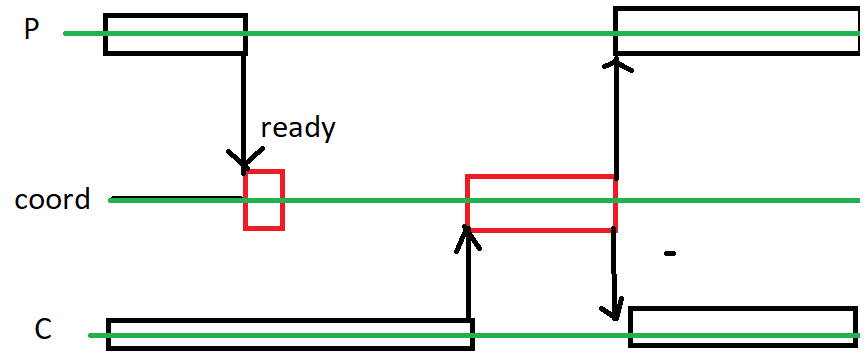
\includegraphics[width=8cm]{sequence.png}
	\caption[Thread activity with an event-handling coordinator.]{TODO. Figure is placeholder too.}
	\label{fig:sequence_diag}
\end{figure}

One pivotal decision of our final design is to attempt to alleviate this problem. If compute-threads are going to block, waiting for progress anyway, why not have them do the coordination \textit{themselves}? In our approach, we discard the dedicated protocol thread and re-interpret the coordinator as a \textit{role} which the other threads take turns adopting. Conceptually, this change is a minor one; there is ultimately still at most one thread acting as coordinator. Until now, we have taken for granted that the coordinator can complete interactions with impunity; as they are the only elected leader of their kind, there is no concern for data races. In our new model, if \textit{anyone} can be a coordinator, we must go our of our way to prevent two threads from adopting the role at once. Where before the bottleneck existed (implicitly) as a single coordinator thread processing a sequence of events \textit{one at a time}, we now make the lock explicit: upon becoming ready, every thread attempts to acquire the \textit{protocol lock}, the holder of which acts is the only coordinator for the duration.

\subsubsection{Delegating the Task of Data Exchange}
Owing to our focus on values at the systems level, we do not have the simplifying luxury of the Java backend to presume that moving data is cheap. In Rust, as in C and C++, values are not represented by indirect references by default; often, their shallowest representations are all there is to them. To satisfy $\boldsymbol{R^N_{data}}$, the Java backend's (admittedly intuitive) representation of ports as data pigeonholes is wasteful. For many realistic Reo protocols, data often moves \textit{through} protocols synchronously, moving from \code{Putter} to \code{Getter} without any storage in memory cells in-between. 

Our implementation introduces a new idea in an attempt to capitalize on this observation: getters fetch their data directly from the \textit{source}. In this approach, the coordinator does necessarily handle data itself. Rather, it decides which rule to fire and \textit{delegates} the task of moving the data to the getters themselves. In addition to skipping a redundant `data hop' from putter to coordinator, this also facilitates the dissemination of a putter's datum to all its getters \textit{in parallel}. This change requires extra messaging form the coordinator, as getters are given more responsibility. Where before a signal from coordinator to getter sufficed (`Your datum is ready!'), coordinators must now communicate the location of the getters' source (`Your datum can be found at $P$!').


\subsection{Architecture}
\label{sec:protocol_object_architecture}
\code{Proto} is a type corresponding closely to its imperative-form specification type, \code{ProtoDef}. While they represent the same thing, their differences in structure and contents are a result of them being used for different \textit{purposes}. Despite the increase in granularity from Reo's RBA-like form, \code{ProtoDef} still represents a \textit{specification} of the protocol; as such, it strives to minimize redundancy to simplify parsing and minimize the surface for internal inconsistency. On the other hand, \code{Proto} is structured to facilitate \textit{execution} at runtime.

\begin{enumerate}
	\item \textbf{Layout optimized for speed.}\\
	As discussed in Section~\ref{sec:imperative_to_rust}, the \code{build} method is the only user-accessible means of constructing \code{Proto} instances. The methods of this type can rely on this to assume that their contents are internally consistent, thereby avoiding the cost of performing many checks at runtime. For example, if a \textit{rule guard} includes an equality check between the values in memory cells $m_0$ and $m_1$, \code{Proto} is able to assume that these cells have the same type; it is safe to use the result of $m_0$'s definition of type-equality.
	
	Additionally, concise structures can be re-arranged such that their layout facilitates less computation time. A general example of this paradigm is caching. Here, a clear example is the replacement with symbolic \textit{names} for ports, functions and memory cells (represented by strings in the \code{ProtoDef} type), using \textit{integers} for keying into vectors, maps and other such structures directly.
	
	\item \textbf{Additional data for primitive concurrency.}\\
	Where \code{ProtoDef} can leave information implicit, \code{Proto} must be explicit. Interface ports require some data structures for storing concurrency primitives. For example, coordinators must send \textit{control messages} to getters, as explained in Section~\ref{sec:chosen_design} above. 
\end{enumerate}

\subsubsection{Critical Region}
Section~\ref{sec:chosen_design} explains how threads initiating actions at boundary ports of a protocol assume the role of coordinator. It is fruitful to examine the fields of \code{Proto} in accordance to which \textit{roles} access them, and how their access is safely controlled. The most coarse-grained distinction is that between fields inside and outside the protocol's lock-protected \textit{critical region}. This divide is so fundamental, that is is immediately apparent by looking at the definition of \code{Proto} itself, seen in Listing~\ref{listing:proto}. \code{ProtoCr} stores all of the fields manipulated only by the coordinator, such as the \textit{allocator}, to which the coordinator delegates the task of storing persistent values. This is explained further in Section~\ref{sec:memory_cells} to follow. Also observe the field responsible for managing which ports are \textit{claimed}. While this is not a task traditionally associated with the coordinator, it's mutually-exclusive access between threads necessitates that this structure is protected by the lock.

\subsubsection{Spaces}
Clearly, \code{ProtoCr} can contain only the data that is not contended by multiple threads. Some structure is still needed for threads to \textit{rendezvous} such that information can be exchanged and actions can be aligned in time. In the Java implementation, the class \code{Port} served two distinct purposes: (1) stored the value being exchanged by two threads, and (2) acted as the rendezvous for putter and getter. As explained in Section~\ref{sec:chosen_design} above, the former of these tasks does not involve the coordinator in Reo-rs. However, the latter is still relevant. To meet this need, \code{ProtoR} associates \textit{space} for every identifier (for ports and memory cells alike). The difference is name exists to distinguish them from ports, to which they are certainly related, but not identical. For every identifier, its \code{Space} contains precisely the data needed for it to communicate with its peers. For ports, this includes a \code{MsgBox}, which serves as a control-message channel from coordinator to compute-thread. Spaces are discussed further in Section~\ref{sec:data_exchange} to follow. 

\begin{listing}[ht]
	\centering
	\inputminted{rust}{proto.rs}
	\caption[Proto type with parts inside and outside the lock.]{Definitions of the most coarse-grained structures of a protocol instance. \code{Proto} is the entry-point, composed of \code{ProtoCr} in the critical section, accessed by only the coordinator, and \code{ProtoR} outside it, accessed by all.}
	\label{listing:proto}
\end{listing}


\subsection{Behavior}
\label{sec:behavior_implementation}
This section explains how the data structures of the \code{Proto} type comes to life at runtime to emerge as coordination according to the protocol with which it was configured. 

\subsubsection{Rule Interpreter}
Unlike the Java implementation, Reo-rs moves the specification of the protocol type very late into the pipeline from Reo to the final application. Rather than relying on Reo to generate \textit{native} application code, in this work we make more extensive use of the \textit{virtualization} pattern. At runtime, the coordinator traverses rules in data form, performing tasks as a rudimentary \textit{interpreter}. The tasks associated with such a \code{Rule} correspond closely to the conceptual interpretation of the imperative form; as such, they are treated like \textit{transactions} at runtime. 

\hl{TODO more detail and talk about temporary variables}


\subsubsection{Minimizing the Bottleneck}
\label{sec:minimizing_the_bottleneck}
Reo-rs shares its centralized locking architecture with the Java back-end. Regardless of whether the coordinator and the thread that performs the role are decoupled, the importance of providing it mutual exclusion is clear; two coordinators in tandem would not be safe in the knowledge that the state does not change between evaluating the guards and changing the state. Methods exist for \textit{fragmenting} protocols such that the locking becomes finer grained as protocols are into sets of smaller ones. As such, the Reo compiler internally produces a \textit{protocol set} as its output, though the work on this feature is ongoing. Nevertheless, we consider this decomposition an orthogonal concern and consider it no farther. Reo-rs embraces this central lock, but takes measures to minimize the duration for which it is held. In this section we discuss these measures and how they work together to help satisfy $\boldsymbol{R^N_{fast}}$. To structure our reasoning, we identify the tasks a coordinator performs from the moment to acquires the lock (accepting its role), to the moment it releases it (relinquishing the role). 

\begin{enumerate}
	\item \textbf{Initialization}\\
	Section~\ref{sec:port_operations} explains how the time spent purely on \textit{overhead} is diminished by avoiding the event-signal interaction used by the Java implementation, necessary to wake a sleeping protocol thread. Once the coordinator has acquired its lock (a task needed in both versions), transitioning into the work of the coordinator is nothing more than the time taken to invoke the \code{coordinate} function call.
	
	\item \textbf{Checking Readiness and Memory State}\\
	Imperative form shares the explicit representation of the \textit{synchronization set} with RBAs, encoding precisely which ports are involved with the firing. Clearly, a rule cannot fire until all ports involved are \textit{ready}. Per port, this is a boolean property which can be represented by a single bit flag. Owing to the simplicity of this data, each of these sets can be represented as a single \textit{bit-vector}, a data structure for which set-operations are exceptionally fast. Reo-rs takes this optimization a step further by extracting another boolean property per memory cell: \textit{fullness}. The idiomatic encoding for memory cells storing data of type \code{T} in Rust would be the \code{Option<T>} type, such that \code{Option::None} represents \textit{emptiness}. Instead, the relevant flags for fullness are extracted, separated from their data and instead coalesced into another bit-vector. With just a handful of fast bit-wise operations, the coordinator is able to quickly detect whether a rule \textit{cannot} fire, as a result of a port not being ready, or a memory cell being full when it should be empty, or empty when it should be full. In practice, the vast majority of cases where a rule's guard is unsatisfied are detected in this step.
	
	
	\item \textbf{Instructions}\\
	Instructions are relatively expensive compared to the other steps in a rule's interpretation. Their cost scales with their complexity, as they can be defined as arbitrarily large and deep formula terms. Even individually, the cost of each operation can be high, as they include arbitrary user-defined function invocations, arbitrary user-defined equality checks, and allocation space for newly-created data objects. Section~\ref{sec:memory_cells} explains how the cost of memory allocation is mitigated such that the allocation itself is amortized to constant time. For the rest of these operations, there is not much that can be done to avoid the cost; for the most part, they would be expensive even if each rule were performed by a native Rust function. Fortunately, the vast majority of rules for Reo connectors require no instructions at all. In practice, Reo connectors tend not to \textit{inspect} the data whose flow they coordinate. The more intrusive the protocol's routing logic becomes, the more it begins to resemble \textit{computation}, a task for which Reo should probably not be optimized. For the protocols without instructions (including \textit{fifo1}, \textit{alternator}, \textit{sequencers}, \textit{sync}, \textit{lossy sync} and more), the support for instruction parsing costs no more than the time to determine that there are zero instructions to execute.
	 
	 \item \textbf{Movements}\\
	 Once a rule is committed, the role of the coordinator is to kick any getters into action, delegating the data exchange to them. Each \textit{movement} encodes one \textit{resource} (\code{Putter} or memory cell) being distributed amongst a set of \textit{recipients} (each a \code{Getter} or memory cell). This meta-interaction is not synchronous; getters may take arbitrary time before waking up and actually participating in the data exchange. This is not the case for memory cells; as part of the \textit{state} of the protocol, this is manipulated by the coordinator only. As such, operations which move values \textit{into} memory (where memory cells act as getters) are performed first. Section~\ref{sec:memory_cells} explains this procedure in more detail. Here, it suffices to say that the movement of memory between memory cells is fast.
	 
	 For port-getters, the coordinator does not move the value itself. Rather, the work is delegated to the compute-thread by sending a \textit{control message} to the getter's \code{MsgBox}. 
	 
	 Usually, the coordinator does not have to interact with the resource (acting as putter) at all. It can rely on getters to `clean up'. The coordinator returns, releasing the protocol lock. The only exception is for movements with \textit{zero getters}. Such cases can represent a resource being destroyed. In these cases, there is no getter to perform the cleanup, and so, the coordinator does it itself. For a \code{Putter}, this is no more than sending a control message, releasing it. For memory cells, this may require running the \textit{destruction} function associated with the memory cell's data type.  Section~\ref{sec:memory_cells} provides more detail on how these are managed.
	 	
\end{enumerate}

\subsubsection{Data Exchange}
\label{sec:data_exchange}

Eventually, each \code{Getter} waiting at their \code{MsgBox} receives a control message from the coordinator, revealing to them the identity of their \textit{resource}. Their task is to locate the corresponding \code{Space} and contend with an unknown number of fellow getters to complete the \textit{movement}. The correctness of this exchange relies on the satisfaction of a number of properties:
\begin{enumerate}
	\item \textbf{One getter cleans up the resource}\\
	Regardless of whether the resource is a \code{Putter} or a memory cell, the set of getters are responsible for cleaning up the resource to finish the interaction. In the case of a putter, this takes the form of sending them a \textit{control message}, notifying them that everyone has finished inspecting their datum and they may return to the caller. Clearly it is unsafe for anyone to release the putter \textit{before} some getter has finished reading the datum; by returning, the putter may \textit{invalidate} the memory region storing the datum.
	
	In the case of a memory cell resource, cleanup takes the form of re-setting its \textit{ready flag} inside \code{ProtoCr}, signifying that the memory cell is in a stable state can again be involved in rule firings. This is necessary as there is no dedicated thread guaranteed to set this flag in future, as is the case for getters and putters. Section~\ref{sec:memory_cells} to follow also explains how these memory cells are \textit{emptied} in these events such that they can again store new values. This manipulates the protocol's state, potentially making new rules' guards satisfiable. As such, this last getter must once again acquire the protocol lock and attempt to \textit{coordinate}.
	
	\item \textbf{At least $N-1$ getters \code{clone}}\\
	Rust generalizes the operation for \textit{replicating} a datum to produce another instance from it. It is idiomatic to rely on the standard trait \code{Clone} with single operation \code{clone} to implement this behavior. This approach covers cases for which there is a non-trivial means of replicating objects; sometimes, performing a bit-wise copy of the structure's shallowest representation is not enough. Consider the example of \code{Arc} (`atomic reference-counted') in Rust's standard library. This type consists of just a pointer to some heap-allocated tuple \code{(refcount, data)}, and is used for shared, reference-counted ownership of \code{data}. For this type, coping the pointer to the tuple is not sufficient. Cloning must \textit{follow} the pointer and increment \code{refcount}.
	
	\item \textbf{One getter \textit{moves} instead of cloning}\\
	Data movements represent the \textit{transmission} of data from source to a set of destinations. Generally, the value is no longer present at the source afterwards. Na\"ively, the original must be \textit{destroyed} to complete the interaction. However, it is wasteful and illogical to replicate an object only to destroy the original. Instead, we wish to \textit{move} a value between threads, much as Rust's move semantics allow the movement of affine types between bindings. This cannot be done in the conventional way, as movement is defined is generally within the context of a single thread and scope. Regardless of Rust's expressiveness, it is nonetheless an \textit{action-based} language, and does not offer the \textit{interaction} we need.\footnote{Rust is able to understand uni-directional movement of values into \textit{new} threads using the same mechanism by which closures can \textit{enclose} variables in their parent scope. More complex types are able to also create their own notions of safe `movement' by composing actions as we suggest in this section. As in our case, they require the use of \code{unsafe}, as by definition the Rust compiler cannot reason about their correctness in the usual way.}
	
	When orchestrated correctly, we are able to implement a safe \textit{move} operation between threads by invoking a pair of \textit{unsafe} operations, one on either end. In \textit{unsafe Rust} it is possible to \textit{copy} a value without influencing the original. If not done correctly, this can easily lead to \textit{double-frees}. On the other hand, it is possible to leak resource memory with \code{forget}, an operation of Rust's standard library which causes the compiler to consider the value \textit{moved} without invoking \code{drop}. These pitfalls should be familiar to C programmers, as \textit{unsafe Rust} gives one the capability to interact with \textit{raw pointers} in a fashion similar to that of C. Together, these actions constitute the inter-thread move primitive we need.
	
	We elaborate our task by requiring an election between getters, such that one is designated the \textit{mover}, and the rest are \textit{cloners}. 
	
	\item \textbf{All clones must be complete before the move}\\
	 It is unsafe to \textit{move} a value before or while performing \code{clone} on the original. Essentially, every data exchange must proceed in two strict phases such that all clones occur in the first, and the move in the second.
	 Consider again the example of type \code{Arc} by examining this sequence of events that results in undefined behavior: (1) \code{Arc} $x$ represented by a pointer to heap region at $p$ is moved to binding $y$. (2) $y$ goes out of scope, it's \code{refcount} is reduced to zero, and so its heap allocation is freed. (3) \code{Arc::clone} is invoked with $x$, which traverses its pointer to memory position $p$, and attempts to increment \code{refcount}. $p$ is no longer allocated, and arbitrary memory corruption ensues. To prevent such cases, Reo-rs must take care to order all clones of some value before it can be moved, as the Rust compiler would do.
\end{enumerate}

Many solutions are possible, but have in common that these getters must exchange some meta-information safely across thread boundaries. Our solution uses a pair of atomic variables for this purpose, \textit{count} and \textit{mover}, initialized by the coordinator a priori to $N$ and \textit{true} respectively. In a nutshell, \textit{mover} is true if no getter has yet claimed the role of mover, which represents both (1) the responsibility to clean up, and (2) the privilege of moving the original value, rather than cloning it. Part of the procedure at large is a \textit{pair} of \textit{elections} between getters to determine a \textit{mover} and a \textit{last} getter. We elect a mover first. The time between the elections gives the losers (the `cloners') the opportunity to clone, safe in the knowledge that the mover will not clean up until they are finished. If the mover is also elected last, they clean up and return immediately, as all clones must already be complete. Otherwise, the mover must await a signal from whomever is last before cleaning up.

This process is complete enough to implement the desired functionality for \mbox{Reo-rs}. However, we identify two important optimization opportunities which have the unfortunate consequence of complicating the data-exchange procedure further.
\begin{enumerate}
	\item \textbf{Not all getters want data}\\
	Getters participating as a result of the \code{get\_signal} operation will not return a value. Clearly these getters cannot avoid participating in the mover-election, as then nobody would clean up. These getters specialize their interactions by participating in the last-election first. The intuition is that if they lose this election, it is safe for them to return without participating in the mover-election; clearly this covers the case of no getters wanting the data. It is also safe to re-arrange these elections in this case; these getters have no intention to \code{clone}, and thus are not a threat to the invariant that required these elections to be ordered in the first place: all clones are complete by the time the last-getter is
	
	\item \textbf{\code{Copy}-types can be replicated without \code{clone}}\\
	Section~\ref{sec:rust_language} explains how \code{Copy} marks types for which have a trivial destructor, and are safe for multiple getters to replicate by \textit{copying} their value bit-wise. This is the case for primitives, and structures composed entirely out of primitives, such as arrays of integers. 
	
	For copy-types, the mover and the \textit{copiers} may copy the original datum in parallel. Afterward, only a last-getter is elected to clean up, safe in the knowledge that all copies are finished.
\end{enumerate}

The full data-exchange procedure is spelled out in Rust-like pseudocode in Listing~\ref{sec:data_exchange} in the Appendix.

% (1) getters invoked by \code{get\_signal}  //
%
%
%Another optimization exists for cases where the data type implements the \code{Copy} trait, communicating that this type has a trivial destructor, and it is perfectly safe for multiple getters to \textit{copy} the data by replicating its shallowest representation in parallel. This is the case for primitives, and structures composed entirely out of primitives, such as arrays of integers. For these types, each getter knows a priori that every getter will conclude that the type implements \code{Copy}, and it can forgo the mover-election business. It is still necessary to elect one getter as the \textit{last} to perform the cleanup (the putter must still be released, or the memory cell must still become ready). The full procedure for a getter's role in data exchange is given in the appendix as Listing~\ref{listing:get_data}, which in and of itself demonstrates the logistic complexities that Reo-rs is able to hide from its users.



\subsubsection{Memory Cells}
\label{sec:memory_cells}
Section~\ref{sec:protocol_object_architecture} explains that per \textit{location} (generalizing ports and memory cells), Reo-rs maintains a persistent \code{Space} structure at a fixed location on the heap such that threads have a predetermined location to \textit{rendezvous} on communication primitives. Section~\ref{sec:data_exchange} follows up, explaining how these structures are also pivotal to data exchange. When getters converge on the space of a \code{Putter}, they rely on the presence of a prepared \textit{data reference} in the space to the location of the putter's datum on its own stack. In this manner, values moving between ports are never moved to the heap at all. The memory-alignment of the putters datum generally differs per data exchange, necessitating that their space's reference be \textit{updated} to the location of their value each time. 

Memory cells differ from putters in that their value \textit{persists} beyond the lifetime of any individual thread participating in the protocol; consequently, the data itself \textit{must} be stored on the heap. A na\"ive implementation treats memory cells similarly to putters by continuously \textit{updating} the data-reference in the associated \code{Space} such that it points to a freshly-allocated value on the heap every time the memory cell is filled.

We are able to rely on a property of Reo for an optimization: memory cells have pre-defined types. Instead of shifting the pointer around to a fresh allocation each time, we are able to \textit{pre-allocate} the space needed to store one value per memory cell. In this model, the references do not change. Instead, each has a single allocation which is repeatedly re-used. Whenever the cell is empty, the contents of the allocated space are \textit{uninitialized}. This can be done safely by relying on auxiliary structures for tracking when memory cells are empty; Section~\ref{sec:minimizing_the_bottleneck} explains how \textit{bit vectors} serve this purpose for Reo-rs. This approach removes the cost of creating and allocating spaces at runtime. Unfortunately, this approach suffers a drawback inherited from its strict interpretation of \textit{value-passing semantics}: moving data between memory cells is expensive. While small optimizations are possible for some circumstances (eg.\ we are able to swap references when the contents of two memory cells are \textit{swapped}), they are only applicable in a handful of situations. 

Requirements~$\boldsymbol{R^N_{data}}$ and~$\boldsymbol{R^N_{fast}}$ incentivize a more extensive optimization. Reo-rs intentionally decouples memory cells (including their spaces and their fullness flags) from \textit{storage}, which describes where the contents of the cells is kept on the heap. We observe that Reo protocols perform logical replication of values often, while mutating existing values rarely. As such, many situations exist in which we are able to safely \textit{alias} values between memory cells by relying on \textit{reference counting}. We extend the idea of re-using allocations, but rather that fixing them per memory cell, we allow all memory cells of the same data type to draw from a shared pool of re-used allocations; this is often referred to as an \textit{arena allocator}. The intricacies of this process are delegated by the coordinator to the \code{Allocator}, which tracks which \textit{storage cells} of a type are available (free) and which are occupied. Rules which replicate, destroy or move data between memory cells thus can often moving data altogether, instead manipulating only the references within spaces, and reference counters of storage cells. For example, a rule which empties memory cell $m_0$ (destroying the contents) needs to only decrement the reference counter. Only when the counter reaches zero does the allocator need to be involved, invoking the value's destructor in-place and freeing the storage slot. This approach has another advantage: \code{clone} is invoked \textit{lazily}, in some cases being avoided altogether. Consider a connector for which values originate from putters, get stored in memory slots, are replicated repeatedly, only to be destroyed before ever being emitted to a getter. In this example, \code{clone} is never necessary. This approach has an additional consequence; the data exchange operation explained in Section~\ref{sec:data_exchange} may be initialized such that \textit{nobody} is permitted to move. The procedure already given (in Listing~\ref{sec:data_exchange}) is able to handle this case.



%
%Memory cells can be \textit{empty}, in which case their pointers are \textit{dangling}\code{For safety, their pointers are managed such that they are \code{null} if and only if the memory cell is empty. This is safe, as null never represents a valid value. Reo-rs can be compiled with \textit{assertions} intact to continuously check this invariant.}. A na\"ive implementation might affix the location
%
%Reo allows the expression of \textit{stateful} protocols whose rules move data into and out of memory cells inside the protocol itself. The protocol object already stores \textit{references} to data on the stacks of port-putters, but this data is \textit{transient}, where memory cells are persistent. To play the part, each protocol object contains a \code{Storage} structure, which acts as a custom \textit{memory allocator}. As the \textit{system allocator} (familiar in C through functions \code{alloc} and \code{free}) depends on a simpler layer of system calls (\code{mmap} etc.) to provide the intended functionality, so too does the \code{Storage} rely on the system allocator. This special type has much the same functionality of the system allocator, but is designed to take advantage of a non-trivial property of Reo protocols: We at most require one allocation per memory cell, and we know the required memory size and alignment ahead of time, as these cells are typed. Thus, \code{Storage} will make a constant number of system-allocations at runtime, re-using the allocated slots as data is moved in and out.
%
%As both the behavior of the coordinator and the allocator are under the control of Reo-rs, it is safe to represent values in memory cells with a layer of indirection between a \textit{memory cell} (a variable that is involved with guards and rules), and \textit{storage cell} (A chunk of memory reserved by the allocator). Regardless of the size of the data itself, `moving' it between memory cells is an instance of \textit{reference passing}.
%
%This approach can be easily extended to facilitate a powerful optimization: \textit{aliasing}. In practice, it is common for Reo to replicate data without mutating either replica. Until the replicas diverge, it is perfectly correct to \textit{alias} the original memory cell by copying its storage-cell reference. Here, the contents of a storage cell are only moved out again if the reference to it is \textit{unique}. This necessitates \textit{reference counting}.
%
%Observe that this approach allows us to \textit{delay} the cost of the \code{clone} operation, avoiding it entirely in cases where the clone is never mutated nor moved out of protocol memory before being discarded; ie. aliased references are made independent with \code{clone} \textit{lazily}. The logical extreme of this idea is to avoid unnecessary clones entirely, covering cases where a value is cloned into memory from a putter, and then discarded. (TODO) Our solution relies on the Reo compiler's minimization procedure to remove these data-movements when the value is \textit{statically} guaranteed to be discarded before use. Supporting the \code{get\_signal} operation described in Section~\ref{sec:port_features} prevents us from avoiding these clones where their values are discarded \textit{dynamically}, as the choice of whether it will be used is not decided until \textit{after} the putter has returned, invalidating the original datum.
%\hl{
%memory cells clearly outlive the stacks of any putters. therefore, the protocol has its own independent persistent memory on the heap. However, it does not use the system allocator directly; data moves through ports very quickly and the overhead of allocating new objects is exceptionally wasteful. instead, we leverage the information made available by the reo specification: we know ahead of time which memory allocations we will need, and we know precisely in which sizes and alignments they will be. we can allocate a fixed number of STORAGE SLOTS and then re=use them. A sensible implementation would simply assign such a slot to each MEMORY CELL SPACE and swap values in and out, initializing and uninitializing the same memory region repeatedly. Clearly, as these memory variables are of irregular sizes, this necessitates a level of indirection: spaces have POINTERS to an allocated heap space. while we are at it, a minor change provides a powerful optimization: we decouple storage slots and memory cells entirely with the addition of a custom ALLOCATOR with REFERENCE COUNTING. when a memory cell moves data to others, only the POINTER moves to its storage slot, and the refcount is updated accordingly. this makes movement and replication within the protocol trivially cheap. it also means that the cost of dropping values is postponed until the last possible moment: the `original' is destroyed only when the LAST memory cell removes its reference.
%}



\subsubsection{Type Reflection}
\label{sec:type_reflection}
\hl{TODO refactor. PortDatum is no longer public-facing}



Section~\ref{sec:rust_language} explains how Rust offers both \textit{static} and \textit{dynamic} dispatch for executing generic code, similar to how it is done for C++. These options offer a trade-off in runtime speed, binary size and flexibility. The interpreter approach taken by Reo-rs makes it difficult to make effective use of static dispatch, as this requires that the concrete type be known at the \textit{call site}. While it is common for Rust libraries to be written in terms of generic arguments which the user will statically dispatch in their own code, this is not particularly ergonomic in our case. As their types are distinguished by context alone, it is impossible to store generic types together in typical collections (such as maps or arrays). This presents a problem for defining objects for generic Reo protocols, which vary also \textit{number} and \textit{arrangement} of data types. 

Cases such as ours which require more extensive flexibility usually rely on dynamic dispatch instead. With this approach, generic type parameters behave less like static \textit{macros}, and more like \textit{interfaces} in Java, whose virtual functions are resolved at runtime. 
As Java interfaces define their virtual functions, Rust achieves dynamic dispatch by hiding some concrete type behind a particular \textit{trait}, which provides the interface henceforth. Appropriately, the Rust term for these dynamic objects is \textit{trait objects}, identifiable by the keyword \code{dyn}, for example, \code{Box<dyn Foo>}. In our case, we define trait \code{PortData} to encapsulate precisely the operations Reo needs: (1) a function for checking equality, (2) an accessor function for the concrete type's \textit{layout}, which allows us to create new heap allocations, (3) the type's destructor, and (4) the associated \code{clone} operation. These type-specific operations are distinguished at runtime by traversing \textit{virtual function tables} of the data types to resolve their specific functions. This lookup incurs some extra overhead at runtime, but we argue why this is acceptable for Reo-rs:
\begin{enumerate}
	\item \textbf{Only pay for what you use}\\
	The most significant argument in favor of dynamic dispatch for our case is the observation that the only significant downside, the added overhead to type-specific operations, are seldom incurred. Much of the work performed by the coordinator is agnostic to the data-type. Section~\ref{sec:data_exchange} explains how usually getters perform moves themselves, while coordinators interact with spaces, send messages and compare bit vectors. Furthermore, usually the argument in favor of reducing overhead is in the context of \textit{hot path} computation; one wouldn't use dynamic dispatch to compute force vectors between every pair of atoms in a physics simulation, as these would dominate the computation. Protocols are low level but simply not \textit{that} low.
	
	\item \textbf{Reduced binary size}\\
	In some cases virtualization is able to \textit{increase} performance indirectly by reducing the overall size and heterogeneity of the binary. When a program has enough different port types, static dispatch would (statically) cause a lot of code replication that interacts poorly with the \textit{instruction cache}.
	
	\item \textbf{Data type can change at runtime}\\
	Dynamic dispatch is a method of relegating the task of distinguishing type behavior to runtime by relying on \textit{data} to distinguish types. Regardless of whether this is done by necessity, this opens up new opportunities for \textit{changing} behavior at runtime. If you change the data, you change the behavior. Projects beyond the scope of this thesis may rely on dynamic dispatch to implement \textit{dynamic reconfiguration}. In a sense, the interpreter approach taken by Reo-rs represents this idea taken to the extreme: changing the contents of the \code{Proto} is able to influence more than just the \textit{types} of protocol rules, but alter them altogether.
\end{enumerate}

Rust's chosen representation of trait objects is the \textit{fat pointer}, which is able to represent an indirect object by appending a \textit{virtual function table} (`vtable'). These two pointers can be thought of as representing the data and behavior respectively. The necessity for the data itself being accessed via indirection is clear; objects implementing the trait may have different sizes in memory, but these sizes must be unified to create a common trait object with a known size. The second pointer is used by Rust `under the hood' to access the concrete functions of the original object such that it's data is accessed by functions of the correct concrete type. These trait objects can be thought to carry their behavior around with them by moving with their vtables. While ergonomic in general, this is often redundant in the case of Reo, where values are guaranteed to only move between ports and memory cells of the same type anyway. In our case, vtable pointers would be repeatedly overwritten by the same vtable pointer, coupled to a new datum. Instead, we split these pointers, and store the vtables at fixed positions; one per memory cell, and some in the \textit{allocator}. In this manner, we are able to use Rust's native dynamic dispatch, but move only \textit{data} around as is done with static dispatch. 

Our internal use of dynamic dispatch is not visible to the user. The API of putters and getters uses \textit{static dispatch} instead, as it is most suitable for the context; port objects retain the same type throughout their lifetimes. We rely on a custom type, \code{TypeInfo}, to bridge the gap. This type serves a dual purpose: (1) it acts as a key, which can be checked for equality, and (2) it \textit{contains} the vtable of the type it represents. Listing~\ref{listing:reflection} shows the \code{TypeInfo::of} function, which is the user's only means of creating new \code{TypeInfo} instances. This function is used by the user themselves to \textit{specify} the types of in the Rust-representation of a protocol's \textit{imperative form}, \code{ProtoDef}. It is used once more inside the \code{claim} function for creating a new \code{Putter} and \code{Getter}, which guarantees that the new port object represents a logical port associated with a matching \code{TypeInfo}.



\begin{listing}[ht]
	\centering
	\inputminted{rust}{reflection.rs}
	\caption[Tricking Rust into exposing a vtable.]{`Tricking' the Rust compiler into retrieving the vtable of a given type \code{T} for dynamic dispatch to virtual functions of trait \code{PortDatum}. The safe cast on line~7 inserts a pointer to a vtable which the compiler will ensure is present in the program text. \code{TypeInfo} structures can later be used for type reflection, by manually appending this pointer to reconstruct the \textit{fat pointers} that Rust natively uses for dynamic dispatch.}
	\label{listing:reflection}
\end{listing}

\code{TypeInfo::of} works by extracting an object's vtable from the text section of the generated binary, which Rust will guarantee is included by virtue of being used. To demonstrate how this works at runtime, we see the assembly generated for the \code{TypeInfo::of} function with an extremely simplified version of \code{PortDatum} consists of only function \code{get\_num}, where \code{u32} implements the trait with \code{fn~get\_num(\&self)~->~usize\{45\}}. Listing~\ref{listing:reflection2} shows the result of compilation where \code{main} returns the \code{TypeInfo} for~\code{u32}. Here, \code{.L\_\_unnamed\_1} shows the text region of the compiled binary containing a 24-byte-long vtable for \code{u32} when dynamically dispatched as implementors of trait \code{PortDatum}. In Rust, all vtables carry information about the type's \textit{layout} (\code{u32} occupies 4 bytes, and must be 4-byte aligned in memory), as well as a pointer to its \code{drop} function for deallocation (which for \code{u32} is trivial, simply returning). The remaining field points to the single function pointer associated with the trait, returning 45 as expected.  

\begin{listing}[ht]
	\centering
	\inputminted{text}{reflection2.rs}
	\caption[Example of assembly generated for extracting a vtable.]{The resulting assembly showing the vtable of type~\code{u32} for dynamic dispatch of trait \code{PortDatum} (here simplified to only having a single function `\code{get\_num}', returning an integer). Function \code{main} is exposed, creating and returning the \code{TypeInfo} of type~\code{u32} using the function shown in Listing~\ref{listing:reflection}. Observe how this function simply returns \code{.L\_\_unnamed\_1}, the vtable of \code{u32}, included by the Rust compiler.}
	\label{listing:reflection2}
\end{listing}


\section{Requirements and Guidelines Evaluated}
\label{sec:requirements_evaluated}
In this section, we give a summary of the means by which the requirements and guidelines of Section~\ref{sec:requirements_defined} are satisfied and adhered to respectively. This section serves as an overview of this chapter at large, motivating its points by referring to the relevant subsections above.


\begin{enumerate}
	\item[$\boldsymbol{R_{value}}$] Values passing through ports preserve value passing. This is achieved even in the presence of reference-passing optimizations `under the table' by leaning on the same philosophy that Rust uses to prevent data races: prohibit mutable aliasing. Objects are only aliased (accessible via multiple bindings) if they should be identical. Section~\ref{sec:port_operations} explains how we prohibit aliasing into and out of the protocol by relying on value-passing port operations. On the other hand, Reo-rs aliases values, but only \textit{until} they are mutated. Section~\ref{sec:memory_cells} explains how memory values are safely aliased. \hl{TODO refer to the section that treats transform functions}
	
	\item[$\boldsymbol{R_{init}}$] Section~\ref{sec:user_facing} explains how users are shielded from the granular initialization procedure by exposing an API with explicit constructor functions \code{build} and \code{claim} of protocols and ports respectively. Protocol objects are extensively customizable by the expressiveness of \textit{imperative form}, with which \code{build} is parameterized. At the same time, these structures are kept internally-consistent by the preservation of invariants, and relying on \code{build} as the only user-facing means of instantiation.
	
	\item[$\boldsymbol{R_{ffi}}$] C and C++ foreign-function interfaces are provided by relying simply declarations with the C ABI where possible. As C cannot support Rust's notion of generics, where necessary, the \code{ffi} module provides generic-free alternatives for data types and functions where generics are represented as data instead. Reo-rs can thus be compiled once into either a statically- or dynamically-linked library for use in these other languages without any additional runtime overhead.
	
	\item[$\boldsymbol{G_{data}}$] Reo-rs facilitates the transmission of any fixed-size data-types by value. This permits but does require data to be heap-allocated. Sections~\ref{sec:data_exchange} and~\ref{sec:memory_cells} explains how Reo-rs has a value-passing API, but relies on reference-passing to minimize the number of times values are moved in memory.
	
	\item[$\boldsymbol{G_{fast}}$] Section~\ref{sec:chosen_design} explains Reo-rs coordinates the actions of multiple threads while minimizing the overhead of inter-thread communications. Section~\ref{sec:minimizing_the_bottleneck} explains how meta-operations are represented such that they can be batched, allowing the coordinator to reduce the overhead of processing rules for firing.
	
	\item[$\boldsymbol{G_{end}}$] Section~\ref{sec:chosen_design} explains how protocol objects are not given their own threads, trivially facilitating termination detection if no ports remain to interact with it. Section~\ref{sec:construction_and_destruction} describes how protocol structures are implicitly cleaned up once all of their ports are destroyed. 
\end{enumerate}
\chapter{Generating Static Governors}
\label{sec:api}

The cumulation of the previous chapters describe a stand-alone contribution to the Reo compiler. We have seen that users are able to generate Rust source code from a Reo specification (Chapter~\ref{sec:imperative_form}) which may be used in conjunction with their own Rust code to behave according to the corresponding protocol specification at runtime (Chapter~\ref{sec:protocol_runtime}). The programmer is able to rely on these protocol objects to constrain the behavior of their program at runtime such that no deviations from the protocol specification may be observed. 

In this chapter, we design the \textbf{governor generator}, a tool to augment the user's Reo-coordinated Rust programs. As with the Reo compiler before, this tool generates a Rust source file from the Reo protocol specification which the user may import as a dependency. Within, a Rust type which corresponds with a \textit{governor}. If integrated into the implementation of the user's components, the Rust compiler will enforce that the user's code does not \textit{inhibit} the behavior of the system at large. In effect, users are provided an ergonomic means to opt-into their Rust compiler enforcing \textit{liveness} properties of their programs. 

Section~\ref{sec:governor_defined} provides the formal definition of \textit{governors}, and how they relate to protocols, components and liveness. Section~\ref{sec:unintended_constraints} describes the problem the \textbf{governor generator} aims to solve from the perspective of a Rust programmer relying on Reo to coordinate their components' communication. Section~\ref{sec:soluition_static_governance} gives a high-level overview of our corresponding solution. Section~\ref{sec:making_it_functional} explains in detail how the \textbf{governor generator} works, concentrating only on what is required to make it minimally-functional. Finally, Section~\ref{sec:making_it_practical} elaborates on the means by which the solution is made ergonomic and practical.

\section{Governor Defined}
\label{sec:governor_defined}
A Reo protocol specification defines which interactions are permitted between its boundary ports. In other words, protocols \textit{constrain} the behavior of any system of which they are a component. This is the result of Reo's semantics, which 
guarantees that the behavior of a system is the composition of its components at any granularity. However, protocols do not prevent their boundary components from adding constraints of their own. As a consequence, the definition of a component viewed in isolation does provide any guarantees on which interactions \textit{are} observable in the system at large. To make this possible, a component needs some knowledge about the behavior of the system beyond its own ports. Fortunately, Reo specifications take us halfway there, as they make explicit which behaviors they permit in an unambiguous form that can be transformed and inspected. To proceed, we define the \textit{governor}.

Protocol $P$ with interface ports $I_P$ defines $G_{P,I_P}$, its governor with respect to its interface ports. $G_{P,I_P}$ shares interface $I_P$ with $P$ itself, and also constrains the interactions between them in the same manner as~$P$. However, all port actions in $G_{P,I_P}$ are the \textit{complement} of those in $P$, ie.\ all \textit{puts} are \textit{gets} and all \textit{gets} are \textit{puts}. $G_{P,I_P}$ characterizes the behavior of a component that, if connected to $P$ with interface $I_P$, would result in a composite system with the same behaviors of $P$ itself. In other words, $G_{P,I_P}$ describes the behavior which $P$ would permit to occur, from the perspective of a component interfacing with \textit{all} of $P$'s ports.

Governors are generalized such that they are defined for any \textit{subset} of a protocol's interface ports, ie.\ a protocol $P$ with interface $I_P$ defines a set of governors $\{G_{P,x} \; | \; x\subseteq I_P\}$. Governors characterize the reverse-oriented behaviors as before, but such that these behaviors are \textit{projected} onto the governor's own interface; \textit{projection} is defined precisely by Baier et al.\ ~\cite{baier2006modeling}, and is explained in Section~\ref{sec:rba_projection} when it is needed. Here, it suffices to say that the behavior as constrained by the governor omits the actions of all ports not in the governor's interface. This captures the intuition that the governor only specifies the interactions of its own boundary ports, not constraining the actions of other ports at all. As such, the behavior of a governor is \textit{at most} as constrained as that of the protocol itself; for every port not included the interface, the governor potentially becomes more \textit{lenient}. This is made clear for the trivial case of a governor with the empty interface, which has no constraints whatsoever.

The utility of this construction is that it provides a means by which a component interfacing with some protocol $P$ with any of its ports may compute \textit{precisely} which behavior the protocol permits. By relying on the fact that protocol objects will facilitate any and all permitted interactions as possible at runtime, this boundary component is able to predict \textit{precisely} the behavior the component that arises from its composition with the protocol. In the simplest case, one is able to enforce that the resulting behavior matches the constraints of the protocol; equivalently, the protocol's boundary components do not contribute any behavioral constraints that the protocol itself did not define already. For such systems, one may understand the entirety of the system's coordination behavior by inspecting the definition of the protocol alone. In these cases, we say that the component is \textit{adherent} to the protocol.

\section{The Problem: Unintended Constraints}
\label{sec:unintended_constraints}
A central tenet of Reo's design is the \textit{separation of concerns}, part of which is the desire to minimize the knowledge a compute component must have of its protocol. In this view, coordinating the movements of data is not a concern relevant to the task of computation. A desirable balance is possible with the observation that protocol objects are able to partially impose protocol adherence on their neighbors; External ports may instigate a \code{put} or \code{get} at any moment, and the protocol will complete them as soon as the protocol definition allows it. In this way, coordinators possess a crucial subset of the features of \textit{governers}: aligning the \textit{timing} of two actions that compose an interaction. Unfortunately, in the properties of the realm of sequential, action-centric programming itself \textit{implicitly} imposes constraints on the behavior of the system: \code{put} or \code{get} block until their interaction is completed, and no subsequent code (potentially, other port operations) will occur until they do. This is beyond the capabilities of the coordinator to influence.

In the context of application development, this has an interesting consequence; the behavior of the system is influenced by the behavior of (potentially) all of its components. This is sensible in theory, but becomes unwieldy in practice. Even small changes to the behavior of a compute component influences the system's behavior in unexpected ways, as we are not used to thinking about synchronous code as a composable protocol, nor are we able to intuit the \textit{outcome} of the composition. For example, Listing~\ref{listing:transform_not} gives the definition of a compute function which a user may write to interact with a protocol. When \code{p} and \code{g} are connected to a \textit{fifo1} protocol (which forwards \code{p} to \code{g}, buffering it asynchronously in-between), it runs forever and the output will be something like:
\begin{verb}
	I saw true. I saw false. I saw true. I saw false. (...)
\end{verb}.\\However, when connected with the \textit{sync} protocol (which forwards \code{p} to \code{g} synchronously), the system has no behavior. The problem is that even though \textit{fifo1} and \textit{sync} have the same \textit{interface}, \code{transform\_not} is \textit{adherent} to the former protocol, but not the latter. By definition, \textit{sync} fires when both \code{p} and \code{g} are ready, but \code{transform\_rot} does not \code{put} until the \code{get} is completed. Once the intricacies of these programs grow beyond a programmer's ability to keep track of these relationships, the composed system may have \textit{unintended} behavior. This property may be obvious at the small scale of this example, but it becomes more difficult the larger and more complex the program becomes. In the worst cases, an innocuous change adds a new constraint such that no next interaction exists, manifesting at runtime as \textit{deadlock}. 


\begin{listing}[ht]
	\inputminted[]{rust}{transform_not.rs}
	\caption[Rust example of a compute component.]{A function in Rust which can be used as a compute component in a system, connected to a protocol component.}
	\label{listing:transform_not}
\end{listing}


%That said, the Reo compiler aims to generate code which describes \textit{eac}
%
%In this section
%
%1. intro to the problem at high level.
%2. you are writing a more complicated component. multiple ports yeah!
%3. oh no its not behaving as expected!
%4. section guide

%\section{Governors Defined}
%\label{sec:governor}
%In this work, we accept that it is necessary to write compute code that has blocking behavior. Rather than attempting to empower the coordinator with the ability to further influence its boundary components, we introduce explicit governors into our applications such that from the protocol's perspective, the components appear to manage themselves. A particular compute component requires a particular governor as the behavior permitted to the compute component is a function of its \textit{interface} with the protocol.
%
%Ultimately, all governors have in common that they enforce adherence to a given protocol on the components they govern. However, governors may differ on \textit{when} and \textit{how} this enforcement manifest. For example, a governor may intercept and filter network messages at runtime, while another checks for deviations \textit{statically} and emitting compiler errors.
%
%In this work, we leverage the unique expressiveness of the Rust language by creating a tool which generates protocol-specific governor code. When used by an application developer, these governors assess the protocol adherence of compute functions \textit{statically}, and prevent compilation if deviations are detected. As such, these governor are absent from the compiled binary.

\section{Solution: Static Governance with Types}
\label{sec:soluition_static_governance}
In this work, we accept that it is necessary to write compute code that has blocking behavior. Rather than attempting to empower the coordinator with the ability to further influence its boundary components, we empower the boundary components with the ability to manage themselves by exposing the behavior of their protocols. Specifically, we create a means by which we are able to generate the relevant \textit{governor} for a given protocol and interface. With this information exposed, we ensure that the implementation is \textit{adherent} to the protocol by prohibiting it from adding any new constraints. Counter-intuitively, this takes the form of \textit{disallowing} the component from performing the `wrong' port operation, as the resulting blocking behavior would inhibit its ability to perform the `right' port operation.

There is a vast possibility space for facilitating this enforcement on the users code given a governor as it is defined in Section~\ref{sec:governor_defined}; any solution that results in protocol adherence is sufficient. A user with a keen eye would be able to check protocol adherence manually by reasoning about the relationship between their component's control flow. Instead, we opt for a more ergonomic approach that leverages a tool the user is guaranteed to have at their disposal anyway: the Rust compiler. Our solution involves the interplay between two novel facets of the Rust language that follow from its \textit{affine type system}; 
\begin{enumerate}
	\item We are able to model the protocol's underlying \textit{constraint automaton} (see Section~\ref{sec:semantic_models}) as a \textit{type-state automaton} (see Section~\ref{sec:type_state}), such that the Rust compiler is continuously aware of the protocol's \textbf{state} throughout control flow of the user's code wrt.\ its execution at runtime,
	
	\item and we are able to protect the API of Reo-rs's \textit{port objects} (see Section~\ref{sec:user_facing}) such that the Rust compiler statically allows their use only if doing so in the current \textbf{state} preserves \textit{protocol adherence}.
\end{enumerate}

From the user's perspective, they are able to opt-into the Rust compiler enforcing protocol adherence in their component code. Concretely, the are able to modify their implementation such that it takes the form of a function with a \textit{signature} as defined in the Rust dependency generated by the \textbf{governor generator}. The user defines the function with \code{put} and \code{get} operations interspersed with arbitrary Rust code as usual. However, any port-operations that would violate protocol adherence will result in the Rust compiler generating a static \textit{type error}; if their implementation is completed without type errors, the user can be certain that their component's behavior at runtime will be \textit{protocol adherent}.
%(1) 
%
%Counter-intuitively, we are able to 

%we introduce explicit governors into our applications such that from the protocol's perspective, the components appear to manage themselves. A particular compute component requires a particular governor as the behavior permitted to the compute component is a function of its \textit{interface} with the protocol.
%
%Ultimately, all governors have in common that they enforce adherence to a given protocol on the components they govern. However, governors may differ on \textit{when} and \textit{how} this enforcement manifest. For example, a governor may intercept and filter network messages at runtime, while another checks for deviations \textit{statically} and emitting compiler errors.

%In this work, we leverage the unique expressiveness of the Rust language by creating a tool which generates protocol-specific governor code. When used by an application developer, these governors assess the protocol adherence of compute functions \textit{statically}, and prevent compilation if deviations are detected. As such, these governor are absent from the compiled binary.

\section{Making it Functional}
\label{sec:making_it_functional}
This section details the workings of the \textbf{governor generator} tool which generates Rust code given (a) a representation of a protocol's RBA, and (b) the set of ports which comprise the interface of the compute component to be governed.

\subsection{Encoding CA and RBA as Type-State Automata}
% How to do type-state pattern for CA and RBA
\label{sec:type_space_automaton}
The \textit{type state} pattern described in Section~\ref{sec:type_state} provides a means of encoding finite state machines as affine types. Their utility is in guaranteeing that all runtime traces of the resulting program correspond to runs in the automaton. For this class of machines, the encoding is very natural, as there can be a one-to-one correspondence between the states of the abstract automaton, and the types required to represent them. This is also the case for transitions and functions; in the worst case, this mapping is one-to-one also. For an arbitrary transition from states $a$ to $b$ with label $x$, a function can be declared to consume the type for $a$, return the type for $b$, and perform the work associated with $x$ in its body.

The encoding is more complicated for CA, where not only states but data constraints must be encoded into types and must interact with transitions. One approach is to treat \textit{configurations} as \textit{states} were treated before by enumerating them into types. For example, the configuration of state $q_0$ with memory cell $m=0$ is represented by type \code{q\_0\_0}, while state $q_0$ with $m=1$ is represented by \code{q\_0\_1}. On a case-by-case basis, one might be able to represent several configurations using one type in the event these configurations are never \textit{distinguished}. For example, a connector may involve positive integers, but only distinguish their values according to whether they are \textit{odd} or \textit{even} and nothing else; in this case \{\code{q\_0\_0}, \code{q\_0\_1}, \code{q\_0\_2}, ...\} may be collapsed to \{\code{q\_0\_odd}, \code{q\_0\_even}\}. For an arbitrary case unique types are needed for every combination of state with every value of every variable. As RBAs are instances of CA, we are able to represent them using the same procedure. As RBAs are used by both the Reo compiler and Reo-rs, they are the model of choice for governors also. 

\subsection{Rule Consensus}
% how to represent choice
\label{sec:rule_consensus}
The protocol works by firing rules at runtime which correspond to those of the RBA which defines its Reo connector. Section~\ref{sec:type_space_automaton} above explains how various compute-components are able to proceed in lockstep with the protocol's RBA in a type-state automaton of their own. For deterministic RBAs, this is easy enough; everyone can trivially know which action occurs \textit{next}, and they can transition through configuration space independently, safe in the knowledge that their representations of the run will stay aligned. This ignores temporary mis-alignments in \textit{time} for transitions in which the compute component does not communicate with the protocol; for these cases, one may work head, leaving the other in a previous state. However, they will catch up eventually when they both reach a transition that involves them communicating (which is ultimately all that matters). This process becomes more complicated when the protocol can reach configurations with \textit{multiple} choices for the next transitions. Without a priori agreement on how these situations are handled, the choice is defined to be nondeterministic. Clearly, all is well as long as all parties agree on this choice; problems only present themselves when compute components and protocols diagree on what may happen next. If the view of a governor are out of sync with its protocol it is generally unable to guarantee that the actions it permits are adherent, or it may prohibit something it ought not to, resulting in unintended constraints of the intended behavior (in the worst case, deadlock). This is a problem of \textit{consensus}. 

  

%Thus far, we have reasoned about operations on RBAs that preserve their ability to simulate the non-silent port actions of the original. However, at runtime the protocol's state will follow a \textit{particular} path, which may not be the only one possible. When two distinct paths branch out from the current configuration, which one should the governor follow such that it can enforce the correct actions? Consider the protocol \textit{fifo2} once again, and observe that from type-state \code{(E,F)}, two rules may be fired next, one firing $A$ and the other firing $B$. The governor must enforce $A$ if and only if the protocol's state goes down the path for $A$, and likewise for $B$. This is an instance of the \textit{consensus} problem; all RBAs in the system must agree on the path taken such that they can proceed in lockstep.

Many means of creating consensus exist. We are able to enforce a \textit{meta-protocol} a priori between governors and protocol such that consensus emerges at runtime. This can be achieved without any overhead by making the decision based only on information statically available. For example, peers may rely on a shared, total \textit{priority} ordering on rules to remove all nondeterministic choice. Many such meta-protocols are possible, each making assumptions about the desired system behavior.

This work takes the approach of statically `electing' the \textit{coordinator} as the leader in every case, and having all governors follow the lead of its arbitrary choice by `asking' it what to do next \textit{dynamically}. This approach is primarily motivated by its \textit{flexibility}; by supporting an arbitrary choice on the part of the protocol, we make the choice itself an \textit{orthogonal} concern for future work. Electing the coordinator in particular as the leader is also somewhat natural; It is only actor in the system with a complete view of the protocol's state, allowing it to make the choice as a function of the state, ie.\ the protocol is capable of making the best-informed decisions.

In terms of implementation, we make a modification to the encoding of our governor's automaton such that it can represent all choices available from a particular configuration. Before proceeding, the governor `collapses' these options to match the choice of the protocol by communicating with the coordinator. Concretely, the Rust function for a rule no longer returns a \textit{particular} type-state token, but rather a \code{StateSet} which enumerates the options. This object is collapsed as a result of calling \code{determine}. Handling the returned variants branches the governor's control flow in a manner akin to a \code{match} (similar to a \code{switch} statement in other languages), with each arm given a single state token to proceed. Na\"ively, this must be encoded as a distinct \code{enum} type with a variant for every possible outcome. Clearly creating new type definitions for every conceivable combination of branches is prohibitively expensive\footnote{Early versions of our implementation indeed enumerated these types with a relatively effective \textit{powerset} construction. However, it was unable to avoid explosion if there simply were many solutions to be found. The nail in the coffin was the changing from the exponential base from~2 to~3 as a result of the modification explained in Section~\ref{sec:user_defined_simplification}.}. Ideally we wish to be able to create enumeration types on-the-fly with precisely the variants needed on a case-by-case basis. Rust provides \textit{tuples} for this purpose in the case of \code{struct} (product types), it has no parallel for \code{enum} (sum types). This feature has been requested for some time~\cite{anon_sum}. If it is supported one day, this may be ideal fore representing these \code{StateSets} with minimal code generation. 

Until anonymous sum types are supported, our solution to the problem of representing the generic \code{StateSet} type relies on Rust's traits to encode the variants as a \textit{tail-recursive} list of nested tuples. Matching the elements of the lists is achieved by repeatedly attempting to match the \textit{head}. Listing~\ref{listing:state_set} shows one possible representation which uses a final \textit{sentinel} list element to make for an ergonomic definition of the \code{StateSetMatch} trait, which provides distinct head-matching behavior for \textit{singleton} lists from that of larger ones. From the user's perspective, \code{StateSet} objects are opaque, and prevent the automaton from proceeding with transitions until the object is collapsed to some usable \code{State} object.

\begin{listing}[h!]
	\centering
	\inputminted{rust}{state_set.rs}
	\caption[Rust implementation of an arbitrary state set.]{Definition of type \code{StateSet}, which acts as an anonymous sum type by encoding its variants as a tail-recursive tuple in its generic argument. Two non-overlapping definitions of trait \code{StateSetMatch} are provided to make the type behave as expected in response to associated method~\code{match\_head}. Function \code{example} demonstrates how the arbitrary number of variants are matched two at a time by repeatedly attempting to match the first element of the list (the head), translating it into a conventional \code{Result} enum which Rust can pattern-match as usual. The result of this match can depend on the contents of field \code{data}, which is instantiated dynamically at runtime by interacting with the coordinator.}
	\label{listing:state_set}
\end{listing}


% representing an indeterminate state-type which will \textit{later} be chosen from the elements of the set. This type is entirely opaque other than a function to code{determine} it. At runtime, \textit{determine} blocks until the governor receives a message from the protocol, communicating a particular choice. For cases where the \code{StateSet} is a singleton, \code{determine} simply unwraps the element. While the decision is made at \textit{runtime}, the type-state automaton exists at runtime. To make this possible, the programmer must provide behavior for each \textit{case}, corresponding to elements of the set, one of which will be chosen by \code{determine}. This use case describes a \textit{sum type}, which is already present in rust as the \code{enum}, a union type with a set of \textit{variants}. However, every new variant set would necessitate the definition of a new enum. This is impractical, as the number of combinations are large. Instead, we implement our own types which behave and appear to the user much like \textit{anonymous sum types} (which do not currently exist in the rust language). This is achieved by relying once again on Rust's trait system to encode \textit{lists} in type-space, using nested tuples. \textit{Matching} of these nested tuple types translates to peeling away tuple layers.

\subsection{Governed Environment}
\hl{TODO}

\section{Making it Practical}
\label{sec:making_it_practical}
With a basic outline for the implementation, we are able to realize some functional, yet na\"ive governors. However, there is a long way to go before these systems can be applied in any realistic scenario. In this section, we explain which problems remain to be solved, whether for the sake of managing complexity, or for the user's ergonomics.

\subsection{Approximating the RBA}
The approach to generating a type-state automaton from an RBA was given in~\ref{sec:type_space_automaton}. Our type-state automaton suffer the same state-space explosion of Constraint Automata, prior to the inclusion of memory (explained in Section~\ref{sec:semantic_models}). We cannot hope to represent realistic programs with this approach alone, as the type-state automata would be wildly unmanageable in its number of states and transitions. In this section, we explain how the type-state automaton is adapted to \textit{approximate} the protocol's configuration space such that we strike a balance between accuracy and simplicity, without any effect on the governor's correctness.

\subsubsection{Data Domain Collapse}
% making RBA automata feasible
\label{sec:approximating_rba}
We abandon the goal of faithfully representing the entirety of the protocol's configuration space in favor of representing an approximation by assuming all data types to be the trivial \textit{unit-type}. With this assumption, memory cells may be in one of two states: (a) empty, (b) filled with `unit'. Converting existing RBAs may see large sub-expressions of \textit{data constraints} becoming constant, including checks for equality and inequality between port values. This assumption is justified by its relation to Assumption~\ref{as:1} from Section~\ref{sec:minimizing_bottleneck}. In this context, it can be understood to mean that \textit{usually}, two configurations that are only distinguished by having different \textit{data values} in memory cells or begin put by putters satisfy precisely the same subset of the RBA's guards. Consequently, they do not need to be distinguished. This simplification greatly reduces the total number of types to encode an RBA's configuration space. However, it is still necessary to consider the possible \textit{combinations} of all empty and full memory cells, requiring potentially $2^N$ types for $N$ cells. Rather than enumerating these types explicitly, we can rely on the \textit{structure} the RBA provides by simply encoding each automaton configuration as a \textit{tuple} of types \code{Empty} and \code{Full}. In a sense, each tuple is indeed its own type, but neither the code generator nor the compiler need to pay the price of enumerating all the combinations eagerly. For example, a configuration of three empty memory cells would be represented by type \code{(Empty,Empty,Empty)}. For brevity, we will henceforth abbreviate these tuples by omitting commas, and shortening~\code{Empty} and~\code{Full} to~\code{E} and~\code{F} respectively.


As before, we are able to represent an RBA rule as a \textit{function} in the Rust language by encoding a configuration change from $q$ to $p$ determines its \textit{declaration} such that it consumes the type-state of $p$ and returns the type-state of $q$. The na{\"i}ve approach of generating functions per type-state is susceptible to the same \textit{exponential explosion} that plagued CAs in the first place. Fortunately, tuple-types have inherent structure which Rust's generic type constraints are able to understand. The use of generics to \textit{ignore} elements of the tuple coincides with an RBA's ability not \textit{ignore} memory values. Consequently only one function definition per RBA rule is required. The way the rule's data constraint manifests is somewhat different, as our function must \textit{explicitly} separate the \textit{guard} and \textit{assignment} parts and represent them as constraints on the parameter-type and return-type respectively. As an example, Listing~\ref{listing:fifo_tsa} demonstrates the type definitions and rule functions for the \textit{fifo2} protocol first seen in Section~\ref{sec:semantic_models} with the associated RBA shown in Figure~\ref{fig:fifo2_rba}. Observe that the concrete choices for tuple elements act as \textit{value checks} for memory cells in either empty or full states. Omission of a check must be done explicitly using a \textit{type parameter} such that the function is applicable for either case of \code{Empty} or \code{Full}, and to ensure the \textit{new} state preserves that tuple element; this causes memory cells to have the expected behavior of \textit{propagating} their values into the future unless otherwise overwritten by assignments. This serves as an example of a case where our simplification coincides with a faithful encoding of the original protocol as \textit{fifo2} never discriminates elements of the data domains of~$A$ and~$B$.


\begin{listing}[ht]
	\inputminted[]{rust}{fifo_tsa.rs}
	\caption[Type state automaton in Rust for the fifo2 connector.]{Type-state automaton for the \textit{fifo2} protocol in Rust. The three latter functions correspond to the three rules seen for the RBA in Listing~\ref{fig:fifo2_rba}. Function bodies are omitted for brevity. Note that \code{M} is not a type, but rather a generic \textit{type parameter} to be instantiated at the call site.}
	\label{listing:fifo_tsa}
\end{listing}



%For the sake of brevity in sections to come, we introduce a more compact syntax for representing \textit{simplified} RBAs as a list of rules, each of which is:
%
%\begin{tabular}{r|rcll}
%	$index$ & $guard$ & $\rightarrow$ & $assignment$ & $ports$ \\
%\end{tabular}
%\\
%where:
%\begin{itemize}
%	\item $index$ is a numeric index to facilitate referring to specific rules in text
%	\item $guard$ is a string of concatenated symbols $g_0g_1g_2 ...$ from alphabet set \{\texttt{E},\texttt{F},\texttt{.}\} such that $g_i$ \textit{guards} the value of the $i$th memory cell. \texttt{.} is \textit{arbitrary} and thus the memory cell is not checked.
%	\item $assignment$ is formatted similarly to $guard$, but determines the \textit{assignment} of memory cells in the next time stamp. Here, \texttt{.} \textit{carries over} the value from the guard for that memory cell.
%	\item $port$ 
%\end{itemize}




\subsubsection{RBA Projection}
% removing silent transitions p1
\label{sec:rba_projection}
When a protocol's interface is provided as-is to a compute component, its model itself (an RBA in our case) defines precisely what it is permitted to do, just with the \textit{direction} of operations reversed; for the component to be compatible, it must put on port $P$ whenever the protocol gets on $P$, and get on port $Q$ whenever the protocol puts on port $Q$. In such cases, the procedure for encoding the RBA described in Section~\ref{sec:approximating_rba} can be applied directly. Otherwise, the interface of a compute component does not subsume the entirety of the interface of its protocol. In such systems, the protocol interfaces with several compute components. Indeed such cases form the majority in practice; compute components tend to only play a small role in a larger system.

The contents of Section~\ref{sec:approximating_rba} are sufficient to generate some functional governors. We consider a system containing protocol $P$ and connected compute component $C$ with interfaces (port sets) $I_P$ and $I_C$ respectively such that $I_P \supseteq{} I_C$. We wish to generate governor $G_C$ whose task is to ensure that $C$ adheres to $P$. As a first attempt, we translate $P$'s RBA to Rust functions and types as-is. We would quickly notice that the RBA's data constraints represent port-operations that are excluded from $I_C$. These interactions involve no actions on $C$'s part; from the perspectives of $C$ and $G_C$, these actions are \textit{silent}. Equivalently, we do not use the RBA of $P$ directly, but consider instead its \textit{projection} onto $I_C$, which \textit{hides} all actions that are not in the interface projected upon. 


\begin{table}
	\centering
	\begin{tabular}{l|ll|}
		rule & guard & assignment \\
		\hline
		0 & $m_0=*$ & $\gapwedge{}m_0'=d_A$\\
		1 & $m_0\neq{}*\gapwedge{}m_1=*$ & $\gapwedge{}m_1'=m_0\gapwedge{}m_0'=*$ \\
		2 & $m_1\neq{}*$ & $\gapwedge{}d_B=m_1\gapwedge{}m_1'=*$ \\
		\hline
	\end{tabular}
	\caption[RBF for the fifo2 connector.]{RBF of the \textit{fifo2} protocol, equivalent to the RBA in Figure~\ref{fig:fifo2_rba}. Formatted with an outermost disjunct per line such that guard and assignment parts per rule are discernible.}
	\label{tab:fifo2_rbf_tsa}
\end{table}

\begin{listing}[ht]
	\inputminted[]{rust}{fifo_tsa_2.rs}
	\caption[Type state automaton in Rust with silent rules.]{Type-state automaton rules which govern the behavior of a compute component with interface ports $\{A\}$ for the \textit{fifo2} protocol. Function bodies list the \textit{actions} which the component contributes to the system. Observe that rules but 0 are silent.}
	\label{listing:fifo_tsa2}
\end{listing}

As an example, we once again generate a governor for a compute-component with interface $\{A\}$ with the \textit{fifo2} protocol. This time the protocol is represented as an RBF in Table~\ref{tab:fifo2_rbf_tsa} to make the correspondence to the generated governor in Figure~\ref{listing:fifo_tsa2} more apparent. Observe that all but one of its rule functions are \textit{silent}, serving no purpose but to advance the state of the automaton by consuming one type-state and producing the next. As demonstrated here, this approach to generating governors is correct, but has two undesirable properties:
\begin{enumerate}
	\item \textbf{API-clutter}\\
	The end-user is obliged to invoke functions which correspond with rules in the protocol's RBA. In many cases, these rules will serve no purpose other than to consume a type-state parameter, and return its successor.
	
	\item \textbf{Protocol Entanglement}\\
	The type-state automaton captures the structure and rules of the protocol's RBA in great detail. This is a failure to \textit{separate concerns}, which further couples the compute component to its protocol. This has the immediate effect of making components difficult to re-use (their implementations are more protocol-specific), as well as making them brittle to \textit{changes} to the protocol, making them difficult to maintain. 
	
\end{enumerate}

\subsubsection{RBA Normalization}
% removing silent transitions pt 2
\label{sec:rba_normalization}
Section~\ref{sec:rba_projection} introduced a procedure for generating governors, but also discussed a significant weakness; all governors are represented by type-state automata based on the original protocol's rules. In this section, we introduce a notion of \textit{normalization} that intends to \textit{specialize} the governors according to its needs such that it is still `compatible' with the protocol's RBA in all ways that matter, but has greatly reduced \textit{api-clutter} and \textit{protocol-entanglement}. 

Let an RBA be in normal form if it has no silent rules. We observe that the presence of silent rules contributes to both api-clutter and protocol entanglement. Ideally, we wish to abstract away the workings of the protocol as much as possible; at all times, the governor only needs to know which actions the component must perform \textit{next}. To make this notion more concrete, we introduce some definitions which build on one another to define the term we need: our normalization procedure should generate an RBA with starting configuration which \textit{port-simulates} the protocol's RBA in its starting configuration:
\begin{itemize}
	\item $Act(r)$ of an RBA state $r$:\\
	The set of ports in $r$ which perform actions (ie: are involved in interactions).
	
	\item \textit{Rule sequence} from $c_0$ to $c_1$ of RBA $R$:\\
	Any sequence of rules in $R$ that can be applied sequentially, starting from configuration $c_0$ and ending in configuration $c_1$.
	
	\item \textit{$P$-final} wrt.\ port set $I$:\\
	A rule sequence of RBA $R$, with \textit{last} rule $r_{last}$ is $P$-final with respect to port set $I$ if $Act(r_{last})\cap{}I=\{P\}$ and for all rules $r$ in the sequence, $r=r_{last} \lor{} Act(r)\cap{}I=\varnothing$.	
	
	\item RBA $R_1$ in config.\ $c_1$ \textit{port-simulates} $R_2$ in config.\ $c_2$ wrt.\ Interface $I$:\\
	If for every $P$-final rule sequence of $R_2$ starting in $c_2$, ending in $c_2'$ there exists some $P$-final rule sequence of $R_1$ starting in $c_1$, ending in $c_1'$ such that $R_1$ in $c_1'$ port-simulates $R_2$ in $c_2'$.
\end{itemize}

The intuition here is that it does not matter how the governor's RBA structures its rules. It is unnecessary for governors to advance in lockstep with the protocol to the extent that they agree on the protocol's \textit{configuration} at all times. It suffices if the protocol and governor always agree on which \textit{actions} the ports in their shared interface do next. Figure~\ref{fig:path_sim} visualizes this idea; observe how the normalized RBA has entirely different transitions (different labels and configurations), but is ultimately able to pair actions of the protocol for ports in its interface with its own local actions.

\begin{figure}[ht]
	\centering
	\footnotesize
	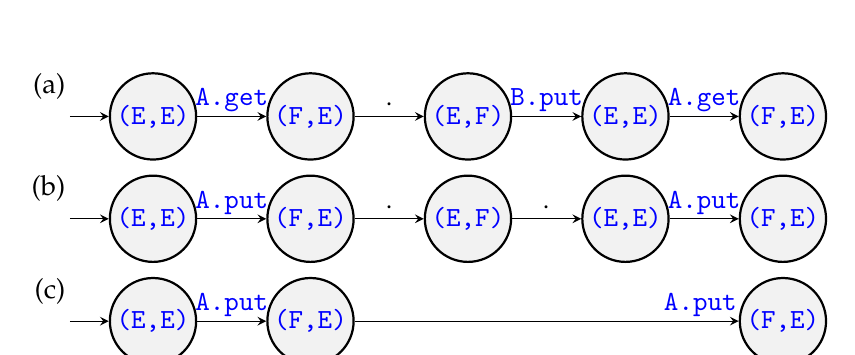
\begin{tikzpicture}[node distance=2cm, inner sep=0.5mm ]
	
	\node[state, initial, initial text=(a)\\\\] (qee) {\code{(E,E)}};
	\node[state, right of=qee] (qfe) {\code{(F,E)}};
	\node[state, right of=qfe] (qef) {\code{(E,F)}};
	\node[state, right of=qef] (qee2) {\code{(E,E)}};
	\node[state, right of=qee2] (qfe2) {\code{(F,E)}};
	
	\node[state, initial, below of=qee, yshift=7mm, initial text=(b)\\\\] (qee') {\code{(E,E)}};
	\node[state, right of=qee'] (qfe') {\code{(F,E)}};
	\node[state, right of=qfe'] (qef') {\code{(E,F)}};
	\node[state, right of=qef'] (qee2') {\code{(E,E)}};
	\node[state, right of=qee2'] (qfe2') {\code{(F,E)}};
	
	\node[state, initial, below of=qee', yshift=7mm, initial text=(c)\\\\] (qee'') {\code{(E,E)}};
	\node[state, below of=qfe', yshift=7mm] (qfe'') {\code{(F,E)}};
	\node[state, below of=qfe2', yshift=7mm] (qfe2'') {\code{(F,E)}};
	
	\draw
	(qee) edge[above] node{\code{A.get}} (qfe)
	(qfe) edge[above] node{$\cdot$} (qef)
	(qef) edge[above] node{\code{B.put}} (qee2)
	(qee2) edge[above] node{\code{A.get}} (qfe2)
	
	(qee') edge[above] node{\code{A.put}} (qfe')
	(qfe') edge[above] node{$\cdot$} (qef')
	(qef') edge[above] node{$\cdot$} (qee2')
	(qee2') edge[above] node{\code{A.put}} (qfe2')
	
	
	(qee'') edge[above] node{\code{A.put}} (qfe'')
	(qfe'') edge[above] node[pos=0.9]{\code{A.put}} (qfe2'')
	;
	\end{tikzpicture}
	\caption[RBAs in lockstep with and without normalization.]{Rules being applied to walk three RBAs in lockstep, with time horizontally, showing the (simplified) configurations traversed, and annotating rules by showing which port actions they involve.\\(a) RBA of protocol \textit{fifo2}. (b) RBA of \textit{fifo2} projected onto port set $\{A\}$. (c) RBA of \textit{fifo2} projected onto port set $\{A\}$ and normalized to remove silent rules.}
	\label{fig:path_sim}
\end{figure}



\begin{listing}[ht]
	\inputminted[]{rust}{normalize.rs}
	\caption[Normalization procedure Rusty-pseudocode.]{Normalization procedure, expressed in (simplified) Rust code. In a nutshell: while one exists, an arbitrary silent rule $x$ is removed, and the list of rules is extended with composed rules $x\cdot{}y$ such that $y$ is another rule.}
	\label{listing:normalize}
\end{listing}

The final normalization procedure is given in Listing~\ref{listing:normalize} in the form of simplified Rust code. It works intuitively for the most part: silent rules are removed, and new rules are added to retain their contribution of moving the RBA through configuration space. The function \code{normalize} ensures that the returned rule set is in the same configuration as the protocol after matching a non-silent, but the configuration is allowed to `lag behind' while the protocol performs rules which it considers to be silent. New rules must be added to `catch up' to the protocol after any such sequence of silent rules. The procedure does this by building these \textit{composed} rules from front to back, ie. replacing every silent rule $x$ with a \textit{set} of rules $x\cdot{}y$, where $y$ is any other rule. Once completed, the RBA may contain rules that are subject to \textit{simplification}. For example, \{$m=*\wedge{}n=*$, $m\neq{}*\wedge{}n=*$\} can be represented by only $n=*$.

The normalization algorithm is \textbf{correct} as clearly it does not have silent rules once it returns (\code{not\_silent} containing zero silent rules is invariant). Observe that for each silent rule removed, it does not consider composing with \textit{itself}. The immediate result is that the algorithm never inserts some rule $x\cdot{}x$ for silent rule $x$. This is not a problem, as all \textit{silent} rules of our approximated RBAs are \textit{idempotent} with respect to their impact on the configuration. The algorithm is able to take for granted that the result any \textit{chain} of silent rules $x\cdot{}x\cdot{}x\cdot{}...$ is covered by considering $x$ itself. Furthermore, the incremental removal of rules prohibits the creation of any silent cycles at all. This is due to the reasoning above being extended to any sequences also\footnote{The reader may note the similarity between this observation and that made by the \textit{pumping lemma for regular languages}~\cite{linz2006introduction}. In both cases, we observe that an arbitrary sequence of `idempotent' cycles as part of a walk through configuration space have no influence on the rest of the path.}. 


The normalization algorithm is \textbf{terminating}. It consists of finitely many \textit{algorithm steps} in which the RBA $A$ is replaced by RBA $B=(A \setminus{}\{r\}) \cup{} \{r\cdot{}x | r\in{} A\setminus{}\{x\} \wedge{} composable(x,r)\}$ for some silent rule $x \in{} A$. Initially, $A$ is the input RBA with silent rules. The algorithm terminates, returning $B$ when $A$ is replaced by $B$ where $B$ has no silent rules. Let $P(x)$ be the set of \textit{acyclic paths} through RBA $x$'s configuration space. Observe that initially, $P(A)$ is finite. It suffices to show that in each algorithm round, $|P(A)|$ strictly decreases. Within a round, for every `added' $p$ in $P(B)\setminus{}P(A)$, $p$ contains a rule $m\cdot{}n$ such that there exists $p'$ in $P(A)\setminus{}P(B)$ identical to $p$ but with a 2-long sequence of rules $m, n$ in the place of $x$. From this we know that $|P(A)| \geq |P(B)|$. However, the 1-long path of $x$ itself is clearly in $P(A)\setminus{} P(B)$. Thus, $|P(A)| > |P(B)|$. \textsc{qed}.

To demonstrate the normalization procedure, Table~\ref{tab:fifo2_rbf_tsa_norm} shows the result of projecting the \textit{fifo2} connector's RBF onto port set $\{A,B\}$ and normalizing. The two additional rules can be understood to `cover' the behavior lost as a result of omitting the silent rule 1 from the original~RBF.


\begin{table}
	\centering
	\begin{tabular}{l|ll|}
		rule & guard & assignment \\
		\hline
		0 & $m_0=*$ & $\gapwedge{}m_0'=d_A$\\
		2 & $m_1\neq{}*$ & $\gapwedge{}d_B=m_1\gapwedge{}m_1'=*$ \\
		\hline
		$1\cdot{}0$ & $m_0\neq{}*\wedge{}m_1=*$ & $\gapwedge{}m_0'=d_A\wedge{}m_1'=m_0$ \\
		$1\cdot{}2$ & $m_0\neq{}*\wedge{}m_1=*$ & $\gapwedge{}m_0'=*$ \\
		\hline
	\end{tabular}
	\caption[RBF of fifo2 connector, projected and normalized.]{RBF of the \textit{fifo2} protocol, projected onto port set $\{A,B\}$ and normalized. Rules 0 and 2 are retained from Table~\ref{tab:fifo2_rbf_tsa}, and new rules $1\cdot{}0$ and $1\cdot{}2$ are composed of rules from the original RBF.}
	\label{tab:fifo2_rbf_tsa_norm}
\end{table}


\subsection{User-Defined Protocol Simplification}
\label{sec:user_defined_simplification}
Recall, the purpose of a governor is to preserve a system's \textit{liveness}.
They do this by ensuring that their governed compute component performs port operations that allow the interfacing protocol (and the system around it) to progress. 
Governors do this by enforcing that their compute component's implementation \textit{covers} each possible transition with code that performs the required task, and ensuring it is chosen correctly in accordance with the wishes of the protocol. Section~\ref{sec:rule_consensus} explains how our type-state automaton represents this by each configuration requiring the definition of a \textit{set} of transitions, one for each action. We say the implementation `covers' each of these cases by defining the component's behavior in each cases, including the invocation of the relevant port operation.

An overzealous governor which requires to cover \textit{additional} (unnecessary) cases would still serve its purpose. In effect, such a governor would enforce adherence to some \textit{other}, more permissive protocol. However, liberty of the protocol means responsibility to the compute-component: the more the protocol \textit{might do}, the more the compute-component \textit{must consider doing}. There is incentive for governors to do this: permissive protocols are simpler to enforce.

This conservatism becomes a problem when it infringes on the component's ability to express its behavior as intended. Consider the example of a compute-component~$X$ that forwards values from its input port~$A$ to its output port~$B$. Perhaps this component is used in a pipeline as intended such that the component is involved in an endlessly-alternating sequence, represented by regular expression~$(AB)^*$. Perhaps there is a sensible way for $X$ to implement the more permissive protocol which permits~$B$ firings to be omitted, expressed $(A(B|\lambda{}))^*$. $P$ has no problem discarding values input from $A$. However, if the governor takes it a step further such that `anything goes' (expressed $(A|B)^*$), $X$~cannot meaningfully represent its work. How on earth can it forward a message to $B$ before receiving it on~$A$? Not even clairvoyance can help; what if $A$ never fires at all? This is how the user would experience the problem of a governor infringing on the component's own behavior; in a sense,~$P$ has a protocol of its own which must be preserved on its interface ports which the governor violates.



\begin{table}
	\centering
	\begin{tabular}{l|ll}
		rule & guard & assignment \\
		\hline
		0 & $m_0=*$
		& $\gapwedge{}m_0'=d_A$\\
		1 & $m_0\neq{}*\wedge{}m_1=*$
		& $\gapwedge{}m_1'=d_A\wedge{}m_0'=*$\\
		2 & $m_0=m_1\neq{}*\wedge{}m_2=*$
		& $\gapwedge{}m_2'=d_A\wedge{}m_0'=m_1'=*$\\
		3 & $m_0=m_1=m_2\neq{}*$
		& $\gapwedge{}d_B=m_0\wedge{}m_0'=m_1'=m_2'=*$\\
		\hline
	\end{tabular}
	\caption{RBF of the \textit{a7b1} connector, which is characterized by cycling through a predictable sequence of period~8, where~$A$ inputs seven times and~$B$ outputs once. It works by encoding its configuration in an 8-long cycle as a three-bit integer using the fullness of memory cells $m_{0-2}$.}
	\label{tab:counting_rbf}
\end{table}

Nevertheless, there is value in providing a compute-component with a simplified (permissive) view of the protocol where possible. As a motivating example, consider the \textit{a7b1} connector, given as RBF in Table~\ref{tab:counting_rbf}. This connector uses the fullness of three memory cells to count in binary from zero to seven (using the binary alphabet of memory cell states $\{\text{\code{E}}, \text{\code{F}}\}$), and cycling back again to zero. Configurations in this cycle are distinguished by specifying different behaviors on~$A$ and~$B$. Here, the projection and normalization of the protocol's RBF is trivial, as no rules are silent. Without the ability to simplify, the~$Y$ must be implemented such that it corresponds exactly with the protocol's (predictable) walk through its approximated configuration space, given in Figure~\ref{fig:counter_RBAs}. As all states are distinguishable, so too are their corresponding \textit{state types} distinct. Now consider this protocol interfacing with some compute-component~$Y$, which is always ready to consume and emit some data element~\textit{Q}. Without simplification, the resulting governor would require that the traversal through configuration space be spelled out; the user would be forced to distinguish these states, even though~$Y$ has no need for this specificity. Most likely, the resulting implementation will be repetitive and verbose, if the behavior is the same for configurations \code{(EEE)}, \code{(EEF)}, et cetera.

\begin{figure}[ht]
	\centering
	\footnotesize
	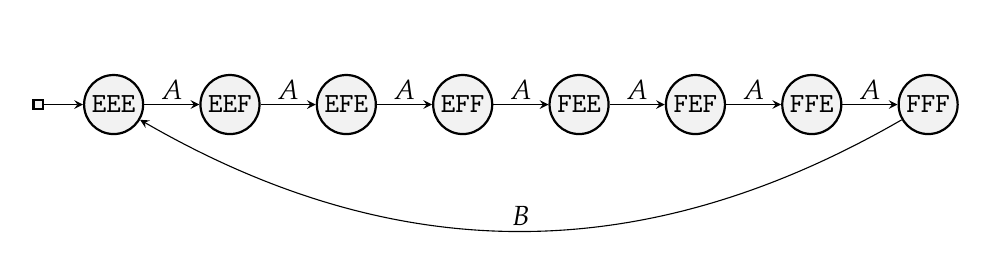
\begin{tikzpicture}
	[ inner sep=0.6mm ]
	\matrix (m) [ matrix of nodes, row sep=0.5cm, column sep = 0.7cm, 
	nodes = {anchor=center,circle, draw=black, thick, fill=gray!10},] {
		\node(m0)[initial]{\texttt{EEE}}; & \node(m1){\texttt{EEF}}; & \node(m2){\texttt{EFE}}; & \node(m3){\texttt{EFF}}; & \node(m4){\texttt{FEE}}; & \node(m5){\texttt{FEF}}; & \node(m6){\texttt{FFE}}; & \node(m7){\texttt{FFF}};\\
	};
	\draw
	(m0) edge[above] node{$A$} (m1)
	(m1) edge[above] node{$A$} (m2)
	(m2) edge[above] node{$A$} (m3)
	(m3) edge[above] node{$A$} (m4)
	(m4) edge[above] node{$A$} (m5)
	(m5) edge[above] node{$A$} (m6)
	(m6) edge[above] node{$A$} (m7)
	(m7) edge[bend left, above] node{$B$} (m0)
	;
	\end{tikzpicture}
	\caption[Configuration space of the a7b1 connector.]{Rules transitioning through configuration space of approximated RBAs for \textit{a7b1} connector, with states named after the `count' the three memory cells represent in base~2 (in binary alphabet $\{\text{\code{E}}, \text{\code{F}}\}$). Here, the normalization procedure with interface set~$\{A,B\}$ is trivial as no transitions are silent.}
	\label{fig:counter_RBAs}
\end{figure}

Our solution to this problem is to introduce a third type for representing the state of a memory cell which may be \textit{either} full or empty:~\code{Unknown} (abbreviated as~\code{U}). Rather than corresponding to a specific configuration of the (approximated) RBA, the governor now reasons about the \textit{set} of states which the protocol may be in. For example, type \code{(UUE)} encapsulates all the concrete configuration types $\{\text{\code{(EEE)}}, \text{\code{(EFE)}}, \text{\code{(FEE)}}, \text{\code{(FFE)}}\}$, and is liable to covering the \textit{union} of the rules applicable to any of those states. In this manner, it is safe for the programmer to arbitrarily `forget' the state of a memory cell, replacing its element in the tuple type with~\code{U}. To be clear, \code{U} is not special as far as Rust is concerned; we have changed to a ternary alphabet for representing memory cells in types. However, \code{U} does not correspond to any real configuration that memory cells are ever `really' in at runtime; they are always either empty or full. \code{U} is a stand-in for an empty \textit{or} full memory variable, an abstraction in which the protocol is not (explicitly) involved.
With this tool in their belt, the implementation of the compute component is able to arbitrarily \textit{unify} the state-types of multiple branches. Our example component~$Y$ above is able to implement its behavior to the satisfaction of its governor with transitions through configuration space in Figure~\ref{fig:weakening}. This weakening can be communicated quite ergonomically, resulting in something very close to what the user would implement themselves: a single loop where the four rules (numbered 0-3) may be applied to configuration type~\code{(UUU)}, each resulting again in~\code{(UUU)}.


\begin{figure}[ht]
	\centering
	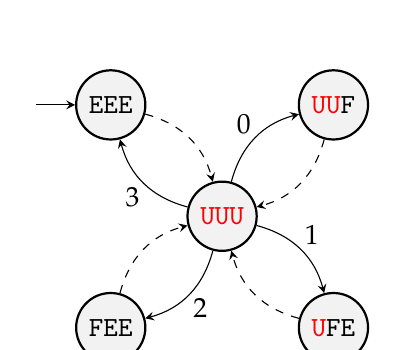
\begin{tikzpicture}[node distance=2cm, inner sep=0.5mm ]
	\node[state, initial]      (q000) {\texttt{EEE}};
	\node[state, below right of=q000] (q???) {\texttt{\textcolor{red}{UUU}}};
	\node[state, above right of=q???] (q??1) {\texttt{\textcolor{red}{UU}F}};
	\node[state, below right of=q???] (q?10) {\texttt{\textcolor{red}{U}FE}};
	\node[state, below left of=q???] (q100) {\texttt{FEE}};
	\draw
%	weakenings
	(q000) edge[dashed, bend left] node{} (q???)
	(q??1) edge[dashed, bend left] node{} (q???)
	(q?10) edge[dashed, bend left] node{} (q???)
	(q100) edge[dashed, bend left] node{} (q???)

%	actual transitions
	(q???) edge[above left, bend left] node{0} (q??1)
	(q???) edge[above right, bend left] node{1} (q?10)
	(q???) edge[below right, bend left] node{2} (q100)
	(q???) edge[below left, bend left] node{3} (q000)
	;
	\end{tikzpicture}
	\caption[Traversed configuration space for a7b1 connector using weakening.]{Rules transitioning between configurations of the \textit{a7b1} connector shown in Figure~\ref{fig:counter_RBAs}. Here, the user employs \textit{weakening} to convert (dashed arrows) state tokens to configurations to the configuration-set `???' containing \textit{all} concrete configurations. RBA rules firing are shown with solid arrows, annotated with the rule name, corresponding to those given in Table~\ref{tab:counting_rbf}.}
	\label{fig:weakening}
\end{figure}



%How can the governor know which distinguishable states the compute components does not wish to distinguish? Our solution is to provide a means for \textit{unifying} 
%We cannot know a priori which distinguishable states the compute component \textit{wishes} to distinguish. Ideally, the user has an ergonomic means of making this choice themselves. Our solution introduces a means for 
%
%
%We currently consider memory variables of the binary domain, ie.\ each is either in state~\code{Full} or~\code{Empty}. We introduce a third state with type \code{Unknown}. Conceptually, configurations with \code{Unknown}-state memory cells represent protocol configurations where each is either concretely full or empty, ie.\ the governor `cannot remember'. 
%
%
%Section~\ref{sec:rule_consensus} describes how the Governor must already be prepared to handle configurations for which there are multiple possible \textit{next} transitions. By adding 
%
%As far as the compiler is concerned, \code{Unknown} is just another state, as distinct from \code{Empty} or \code{Full} as any other. Conceptually, we use \code{Unknown} to represent th
%
%type for a new state memory cells can be in to supplement existing types \code{Empty} and~\code{Full}:~\code{Unknown}. A type-state with memory cells in an \textit{unknown} state is obliged to cover the \textit{union} of all its concrete possibilities. For example, \code{(Empty, Unknown)} may result in any states either \code{(Empty, Empty)} or \code{(Empty, Full)} may result in. With this definition, it is perfectly correct for a state-type to be `weakened', converting it into a new state-type, identical but with any of its tuple-elemets replaced by \code{Unknown}. In a sense, this approach has type-states no longer corresponding with configurations 1-to-1, but rather, each type-state encodes a simple predicate such that it represents a \textit{set} of configurations. For example, \code{(Unknown, Unknown)} represents \textit{any} configuration (of an RBA with two memory cells). Conceptually, this change has no influence on the way a governor computes which rules are applicable next, but the programmer is empowered with the ability to trade \textit{specificity} for \textit{brevity} in their compute-component implementations. Figure~\ref{fig:weakening} shows an example of how the programmer may choose to traverse their configuration space for the same connector as in the example above. In this case, using \textit{weakening} does not reduce the number of type-states encountered in the implementation; this is only the result of (a) the original RBA not being very complicated, and (b) the choice to only \textit{partially} weaken some states (It is also possible to weaken everything to \code{(Unknown, Unknown, Unknown)} and then match all rules).
%
%
%\begin{figure}[ht]
%	\centering
%	\begin{tikzpicture}[node distance=2cm, inner sep=0.5mm ]
%	\node[state, initial]      (q000) {\texttt{000}};
%	\node[state, right of=qee] (q??0) {\texttt{\textcolor{red}{??}0}};
%	\node[state, right of=q??0] (q??1) {\texttt{\textcolor{red}{??}1}};
%	\node[state, below of=q??1] (q?11) {\texttt{\textcolor{red}{?}11}};
%	\node[state, right of=q??1] (q101) {\texttt{101}};
%	\draw
%	(q000) edge[dashed] node{} (q??0)
%	(q??0) edge[above] node{0} (q??1)
%	(q??1) edge[below, bend left] node{3} (q000)
%	
%	(q??1) edge[left, bend right] node{$1\cdot{}0$} (q?11)
%	(q?11) edge[dashed] node{} (q??1)
%	
%	(q??1) edge[below, bend right] node{$2\cdot{}0$} (q101)
%	(q101) edge[dashed] node{} (q??1)
%	;
%	\end{tikzpicture}
%	\caption{Rules transitioning between configurations of the \textit{8-count cycle} connector in Figure~\ref{fig:counter_RBAs}. Here, the user employs \textit{weakening} to convert (dashed arrows) state tokens to configurations with \textit{unknown} memory cell states. RBA rules firing are shown with solid arrows, annotated with the rule name, corresponding to those given in Table~\ref{tab:counting_rbf}. Note that not all possible weakenings are shown, only an example set that covers all rules.}
%	\label{fig:weakening}
%\end{figure}


\subsection{Match Syntax Sugar}
Section~\ref{sec:rule_consensus} explains how the set of transitions to be covered by a configuration type can be represented in Rust's type system as a tail-recursive list. This alleviates the problem of having to explicitly enumerate the needed sets each as their own enumeration type. This is necessary, as the upper-bound\footnote{Many factors reduce this number drastically in practice. For example, state-sets are usually not large because they are only ever encountered when reached by \textit{transitions} from some state.} of state sets is $2^{3^M}$, where $M$ is the number of memory cells\footnote{The number of unique state sets is $2^S$, where $S$ is the number of configurations (automaton state types). This, in turn is $3^M$, as each memory cell's state is represented by a type in $\{\text{\code{E}}, \text{\code{F}}, \text{\code{U}}\}.$}; suffice it to say, it is \textit{a~lot}.
Unfortunately, these are not natively-supported enumeration types, and thus cannot be \textit{matched} as is idiomatic in the Rust language. However, Rust has extensive support for abstract syntax tree \textit{macros}, allowing us to have the best of both worlds; the user interacts with \code{StateSet} types by using a match-like macro which enumerates the branches, but there is no need for concrete \code{enum} classes to be defined for all the conceivable combinations. Figure~\ref{listing:sugar} gives an example of how these cases compare to one another.


\begin{listing}[ht]
	\centering
	\inputminted{rust}{sugar.rs}
	\caption[Example of mimicing enum matching with a sugaring macro.]{Example of three methods for matching a \textit{state set}, representing a sum type of three variant types simplified here to \code{X}, \code{Y} and \code{Z}. First, \code{match\_standard} shows how this is done in idiomatic Rust, requiring an enum type \code{StateSetXyz} be explicitly defined. \code{match\_recursive} shows how the same state set represented by a tail-recursive \code{StateSet} type can be similarly matched by exhaustively `unzipping' head elements using a function \code{match\_head}. finally, \code{match\_macro} functions identically to the second case, but relies on a sugaring macro \code{match\_set} to mimic the syntax of Rust's \code{match} statement, seen in the first function.}
	\label{listing:sugar}
\end{listing}
\chapter{Benchmarking}
\label{sec:benchmarking}

In this section we evaluate the performance of the Reo-rs library, focusing primarily on the optimizations described in Section~\ref{sec:protocol_runtime}.
\hl{TODO add references to requirements and guidelines from Reo-rs chapter}

\section{Experimental Setup}
\hl{TODO}
rustc 1.38.0-nightly (bc2e84ca0 2019-07-17)
compatible and contemporary with rust version 1.36.0 (a53f9df32 2019-07-03)
Windows 10.0.2.1000 intel core i7-7500U CPU @ 2.70 GHz. 12Gb ram, 4 physical (8 logical) 64-x86 architecture processor. Micron 1100 SATA 5122 GB SSD 



%\begin{landscape}
%\begin{table}[p!]
%\begin{adjustbox}{width=19cm}
%\rowcolors{2}{gray!13}{white}
%\begin{tabular}{l|ll|p{46mm}p{67mm}}
%\rowcolor{gray!26}
%Name & Connector & Data Type & Goal & Description \\
%
%\hline
%seq-fifo & fifo1 & Integer & Tease out Proto overhead & alternate between putting and getting on single thread. measure RTT. Repeat for different sizes of data. Compare overhead to std::spsc channel \\
%
%SIMO clone & N-replicator & BigClonable & check if getters are effectively cloning in parallel & repeatedly clone from a single putter in parallel \\
%
%SIMO copy & N-replicator & BigCopyable & check if copying saves a lot of time vs cloning & repeatedly copy from a single putter in parallel \\
%
%MO clone & N-keeper & BigClonable & Check if waiting for putter adds significant time & repeatedly clone from a memcell \\
%
%counting & binary counter & BigClonable & Check how effective the refcounting is & binary counter circuit, moving memory between cells a hell of a lot. not much firing \\
%
%MO fine & N-keeper fine & BigClonable & Check if coordinator is the bottleneck & have one rule per getter. each readiness causing a firing. \\
%
%bitsets & N-keeper fine & BigClonable & fire every time, but after N-1 false guard evals by bitsets & N-keeper where only the last port and rule are active. effectively have to traverse all these dead rules each time \\
%
%hashsets & N-keeper fine & BigClonable & check if the bitsets themselves helped & repeat bitset experiments, but modify Reo-rs to use stdlib hashsets instead \\
%
%transform & transformer & int, float & overhead of createfromcall & \\
%
%filter & filter & int & & \\
%
%router & router & int & & \\
%
%parallel & parallel & BitCopyable & concoct a scenario where data is moving in parallel as much as possible. & 
%
%\end{tabular}
%\end{adjustbox}
%\caption[TODO]{TODO}	
%\end{table}
%\end{landscape}

\section{Reo-rs in Context}
This section compares the performance of Reo-rs to its various competitors: (1) existing Reo back-end for the Java language (2) Hand-crafted Rust protocol code. The goal is to provide the reader with an understanding on the strengths and weaknesses of Reo-rs in a broader context.

\subsection{Versus the Java Implementation}
We begin by making the most intuitive benchmark to get an understanding of how effectively Reo-rs has been optimized for its task; we compare it to the work of the Reo compiler's Java code-generator. This comparison spans two vastly different systems with different goals, but also compare a memory-managed language to a system's language. The reader should bear this in mind when interpreting the measurements. As our test scenario, we have a set of $N$ getters repeatedly copying some memory value $M$, retained inside the protocol from initialization. By involving a contended resource, we are able to test and compare the \textit{scalability} the generated programs, both in terms of number of ports and the size of the transmitted data.

\begin{figure}
	\centering
	\makebox[\textwidth][c]{
		\begin{subfigure}[b]{0.63\textwidth}
			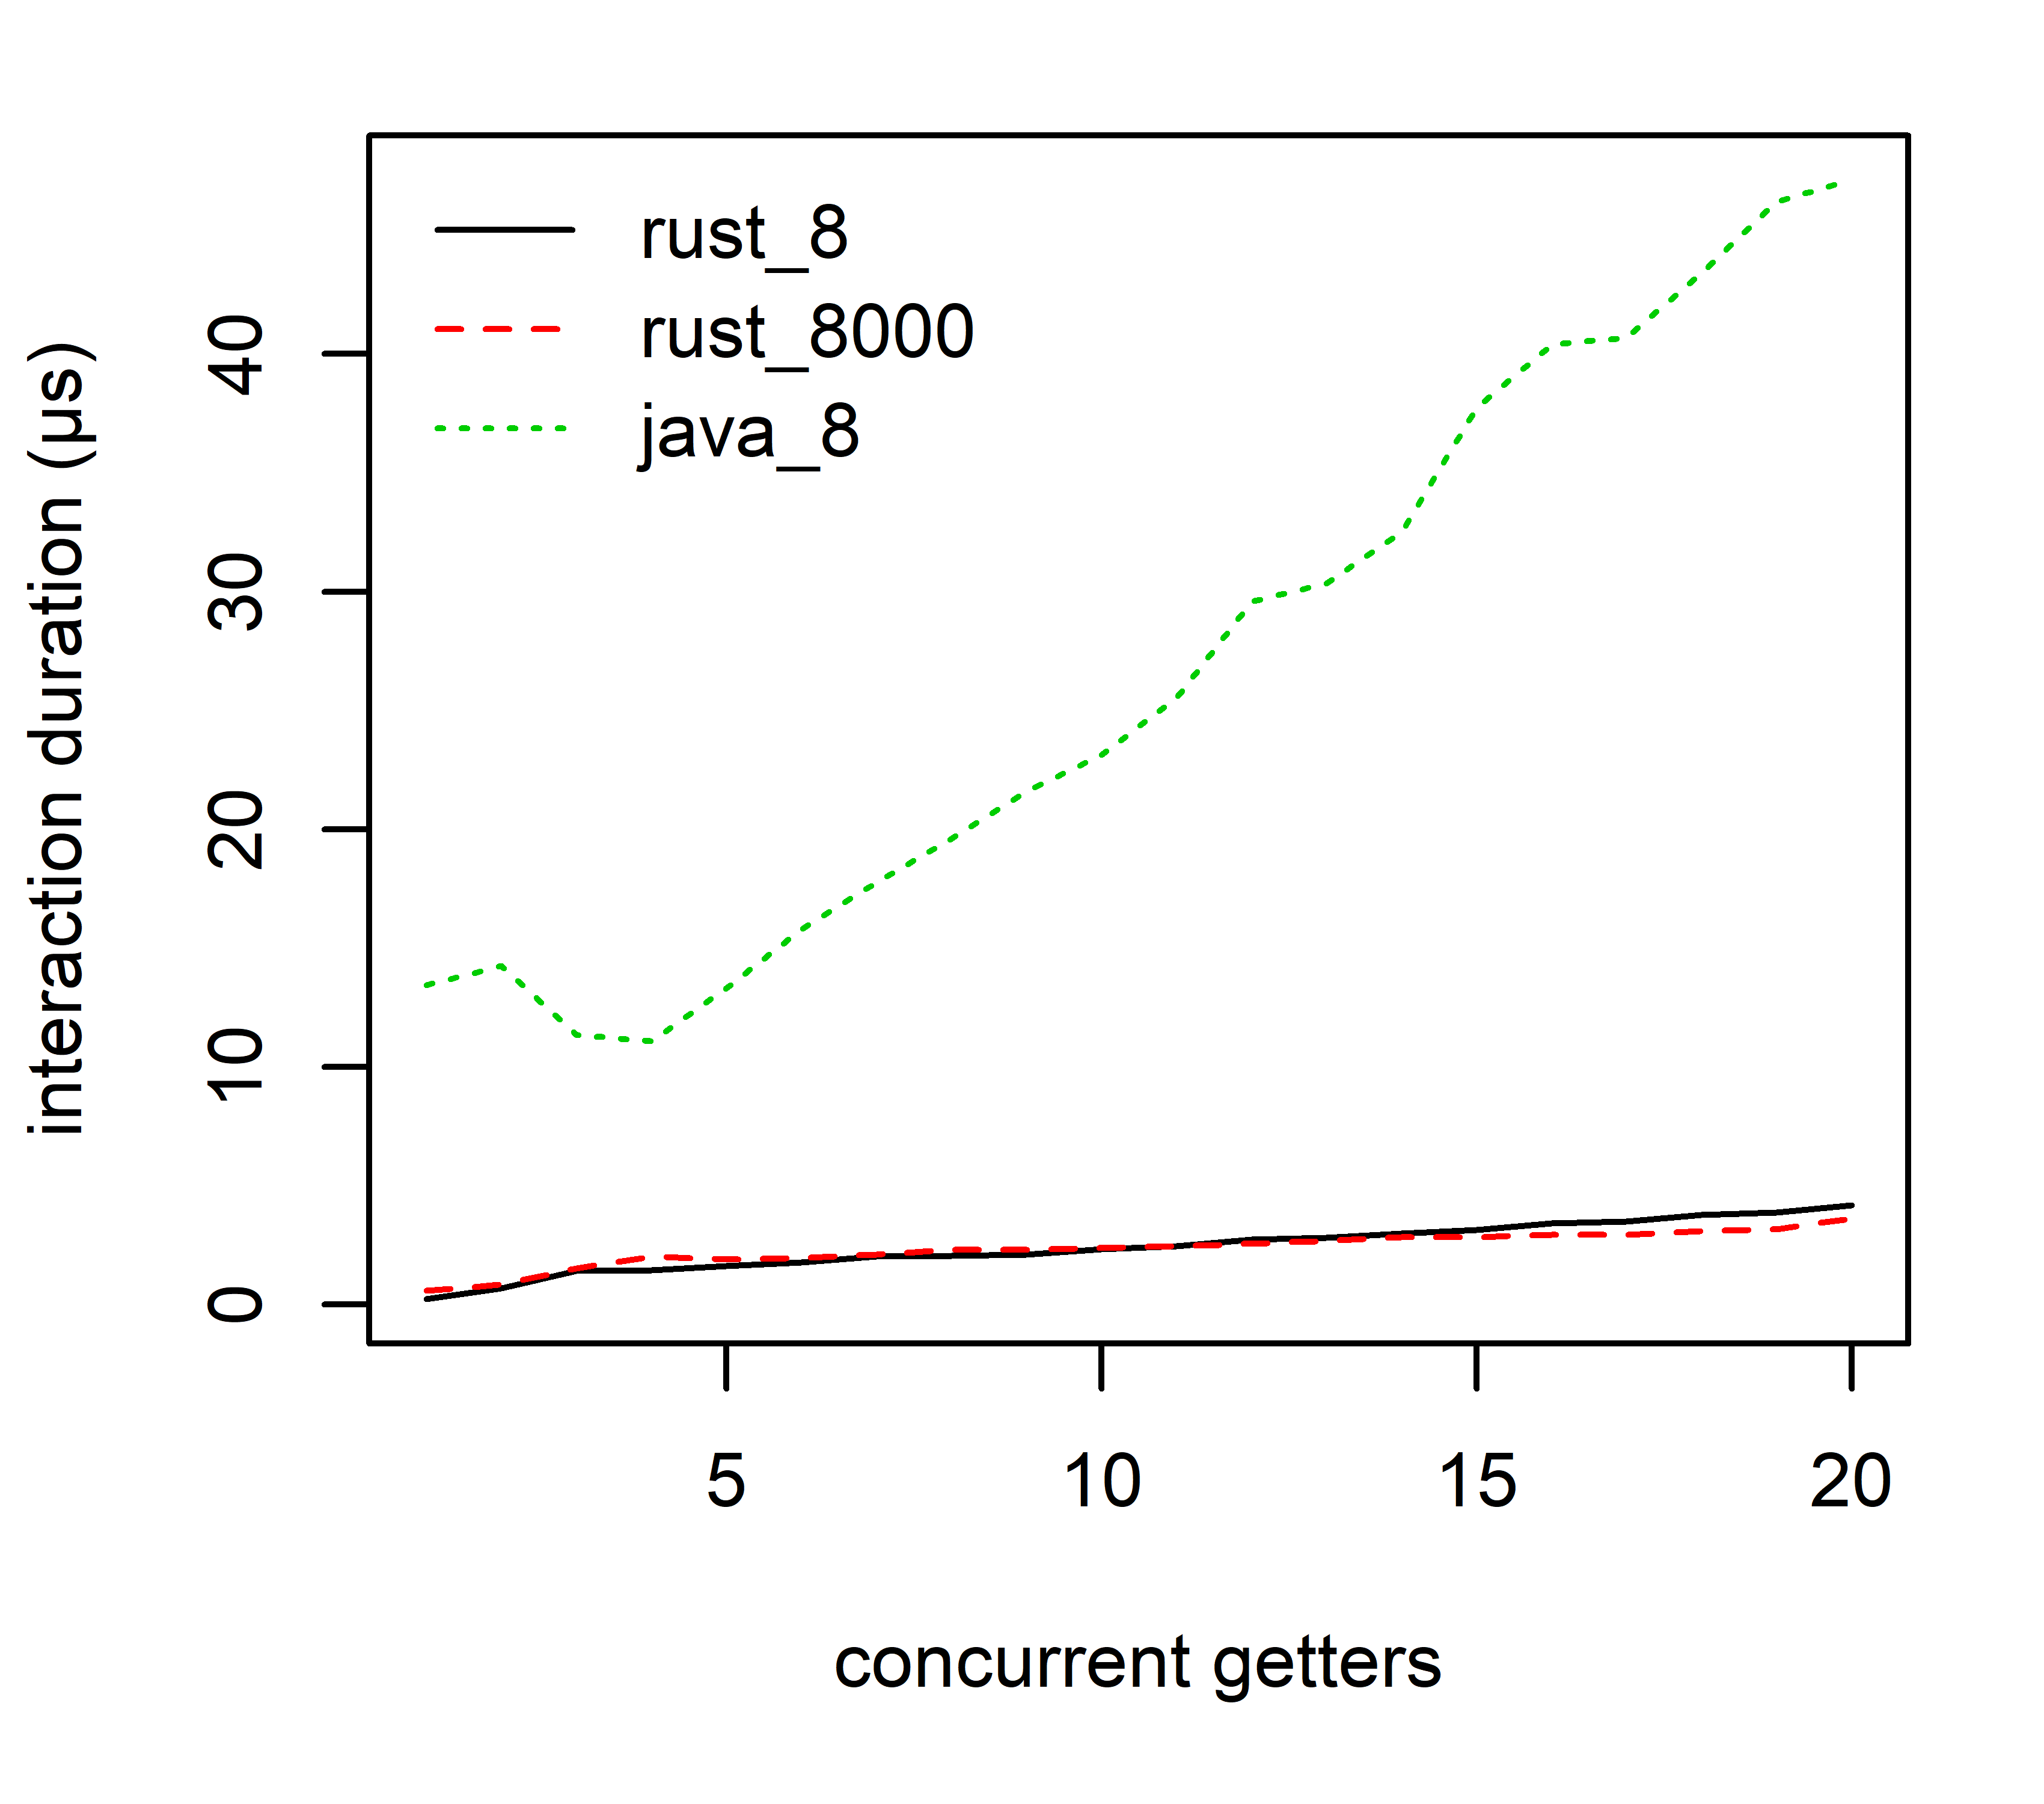
\includegraphics[width=\textwidth]{experiments/rust_v_java_0.png}
			\caption{}
			\label{fig:rust_v_java_0}
		\end{subfigure}%
		\begin{subfigure}[b]{0.63\textwidth}
			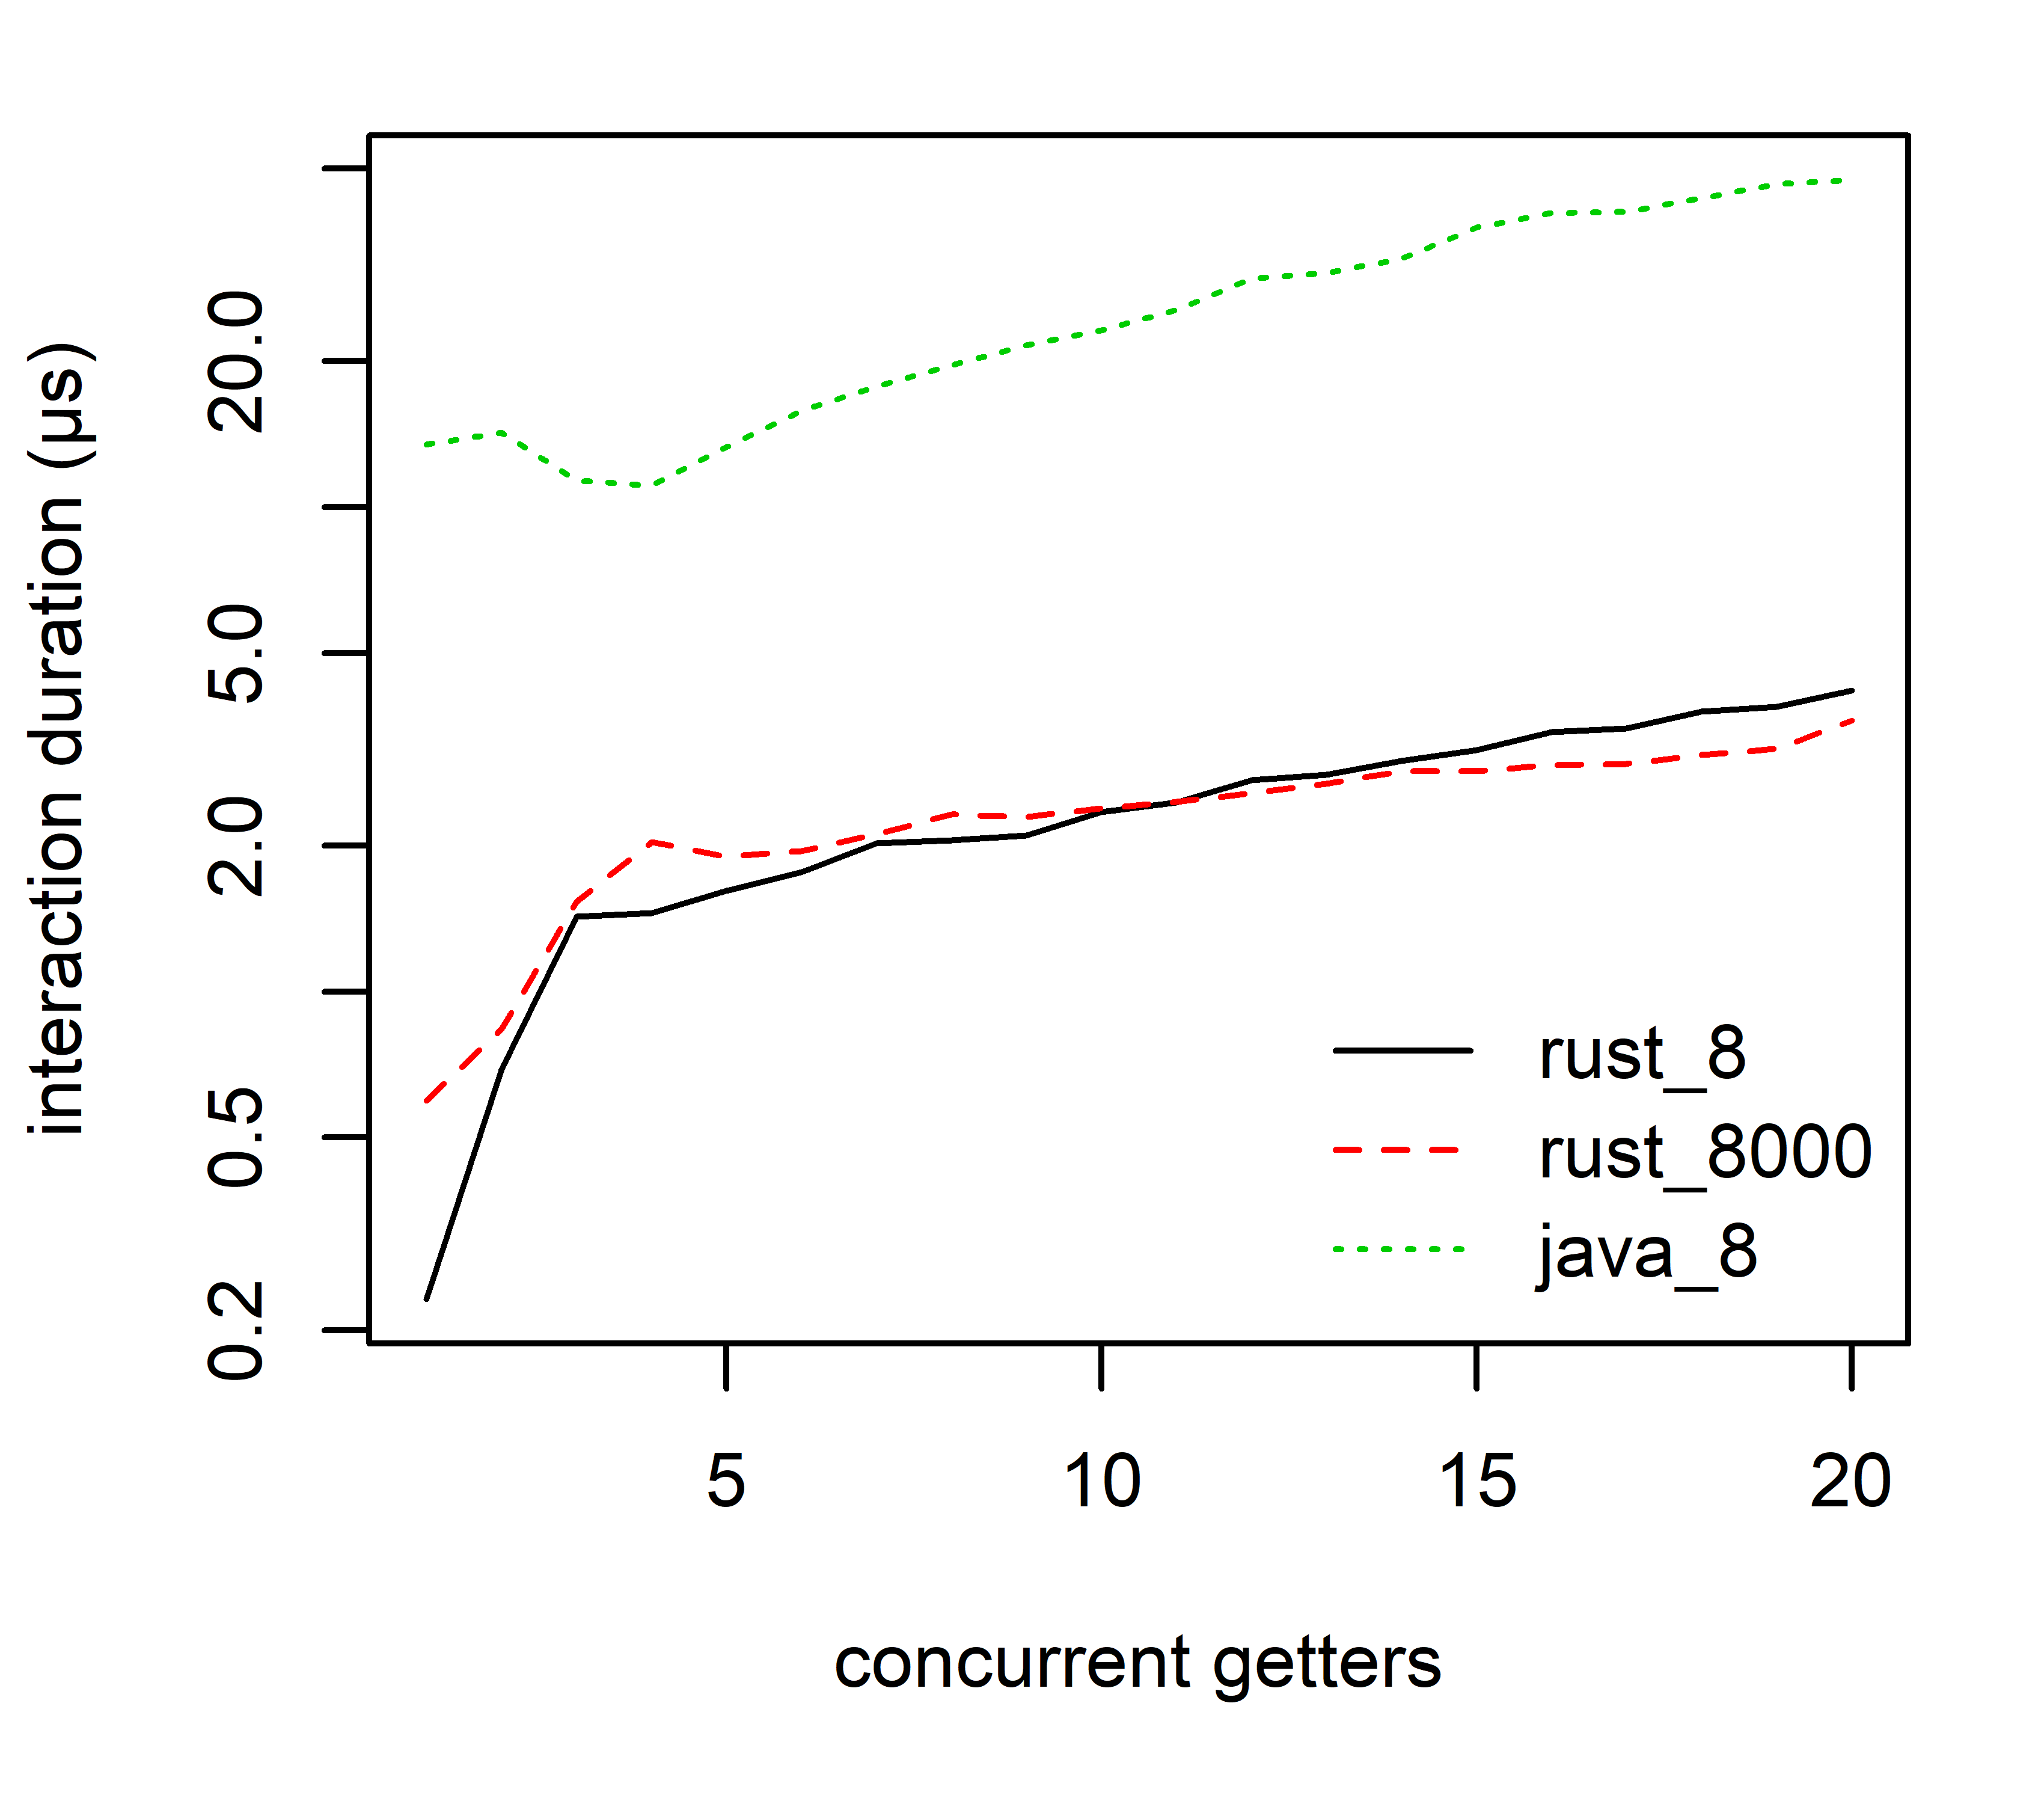
\includegraphics[width=\textwidth]{experiments/rust_v_java_1.png}
			\caption{}
			\label{fig:rust_v_java_1}
		\end{subfigure}%
	}
	\caption[Java vs.\ Rust interaction time for small values.]{Comparison of interaction time for the \textit{fetch} connector for both Java and Rust backends moving small-size values. `rust\_8' and `java\_8' both move a payload of 8~bytes (to match the reference size of the 64-bit JVM). `rust\_8000' gives an example of how the runtime of Reo-rs can change with respect to modest changes in data size. The two sub-figures mirror one another except for the linear and logarithmic y-axes respectively.}
	\label{fig:rust_v_java}
\end{figure}

The unfairness of our comparison cuts both ways, as there is not a clear means of comparing the transmission of large values; the Java version relies entirely on object-aliasing, effectively implementing different semantics. For Java, the size of values transmitted is largely irrelevant. We begin by a comparison on the only common ground; Figure~\ref{fig:rust_v_java_0} shows both Java and Rust are transmitting pointer-sized objects. Aside from the order of magnitude difference in runtime, we observe a different \textit{shape}. Reo-rs is observed to be significantly faster for a single-getter case. This is easy enough to explain; the type relied upon for protecting the coordinator's \textit{critical region} is \code{Mutex} from the \code{parking\_lot} crate, which provides implementations of these kinds of concurrency primitives. \code{Mutex}~is documented as having a \textit{fast path} optimization for when the lock is acquired \textit{uncontested}. Runs with one getter are thus able to take advantage of this optimization every time.

Figure~\ref{fig:rust_v_java_2} attempts to draw the same comparison as before, but in the case of large data-types. The Java-generated protocol objects do not do true value-passing. It is out of the scope of this project to attempt to implement this

\begin{figure}
	\centering
	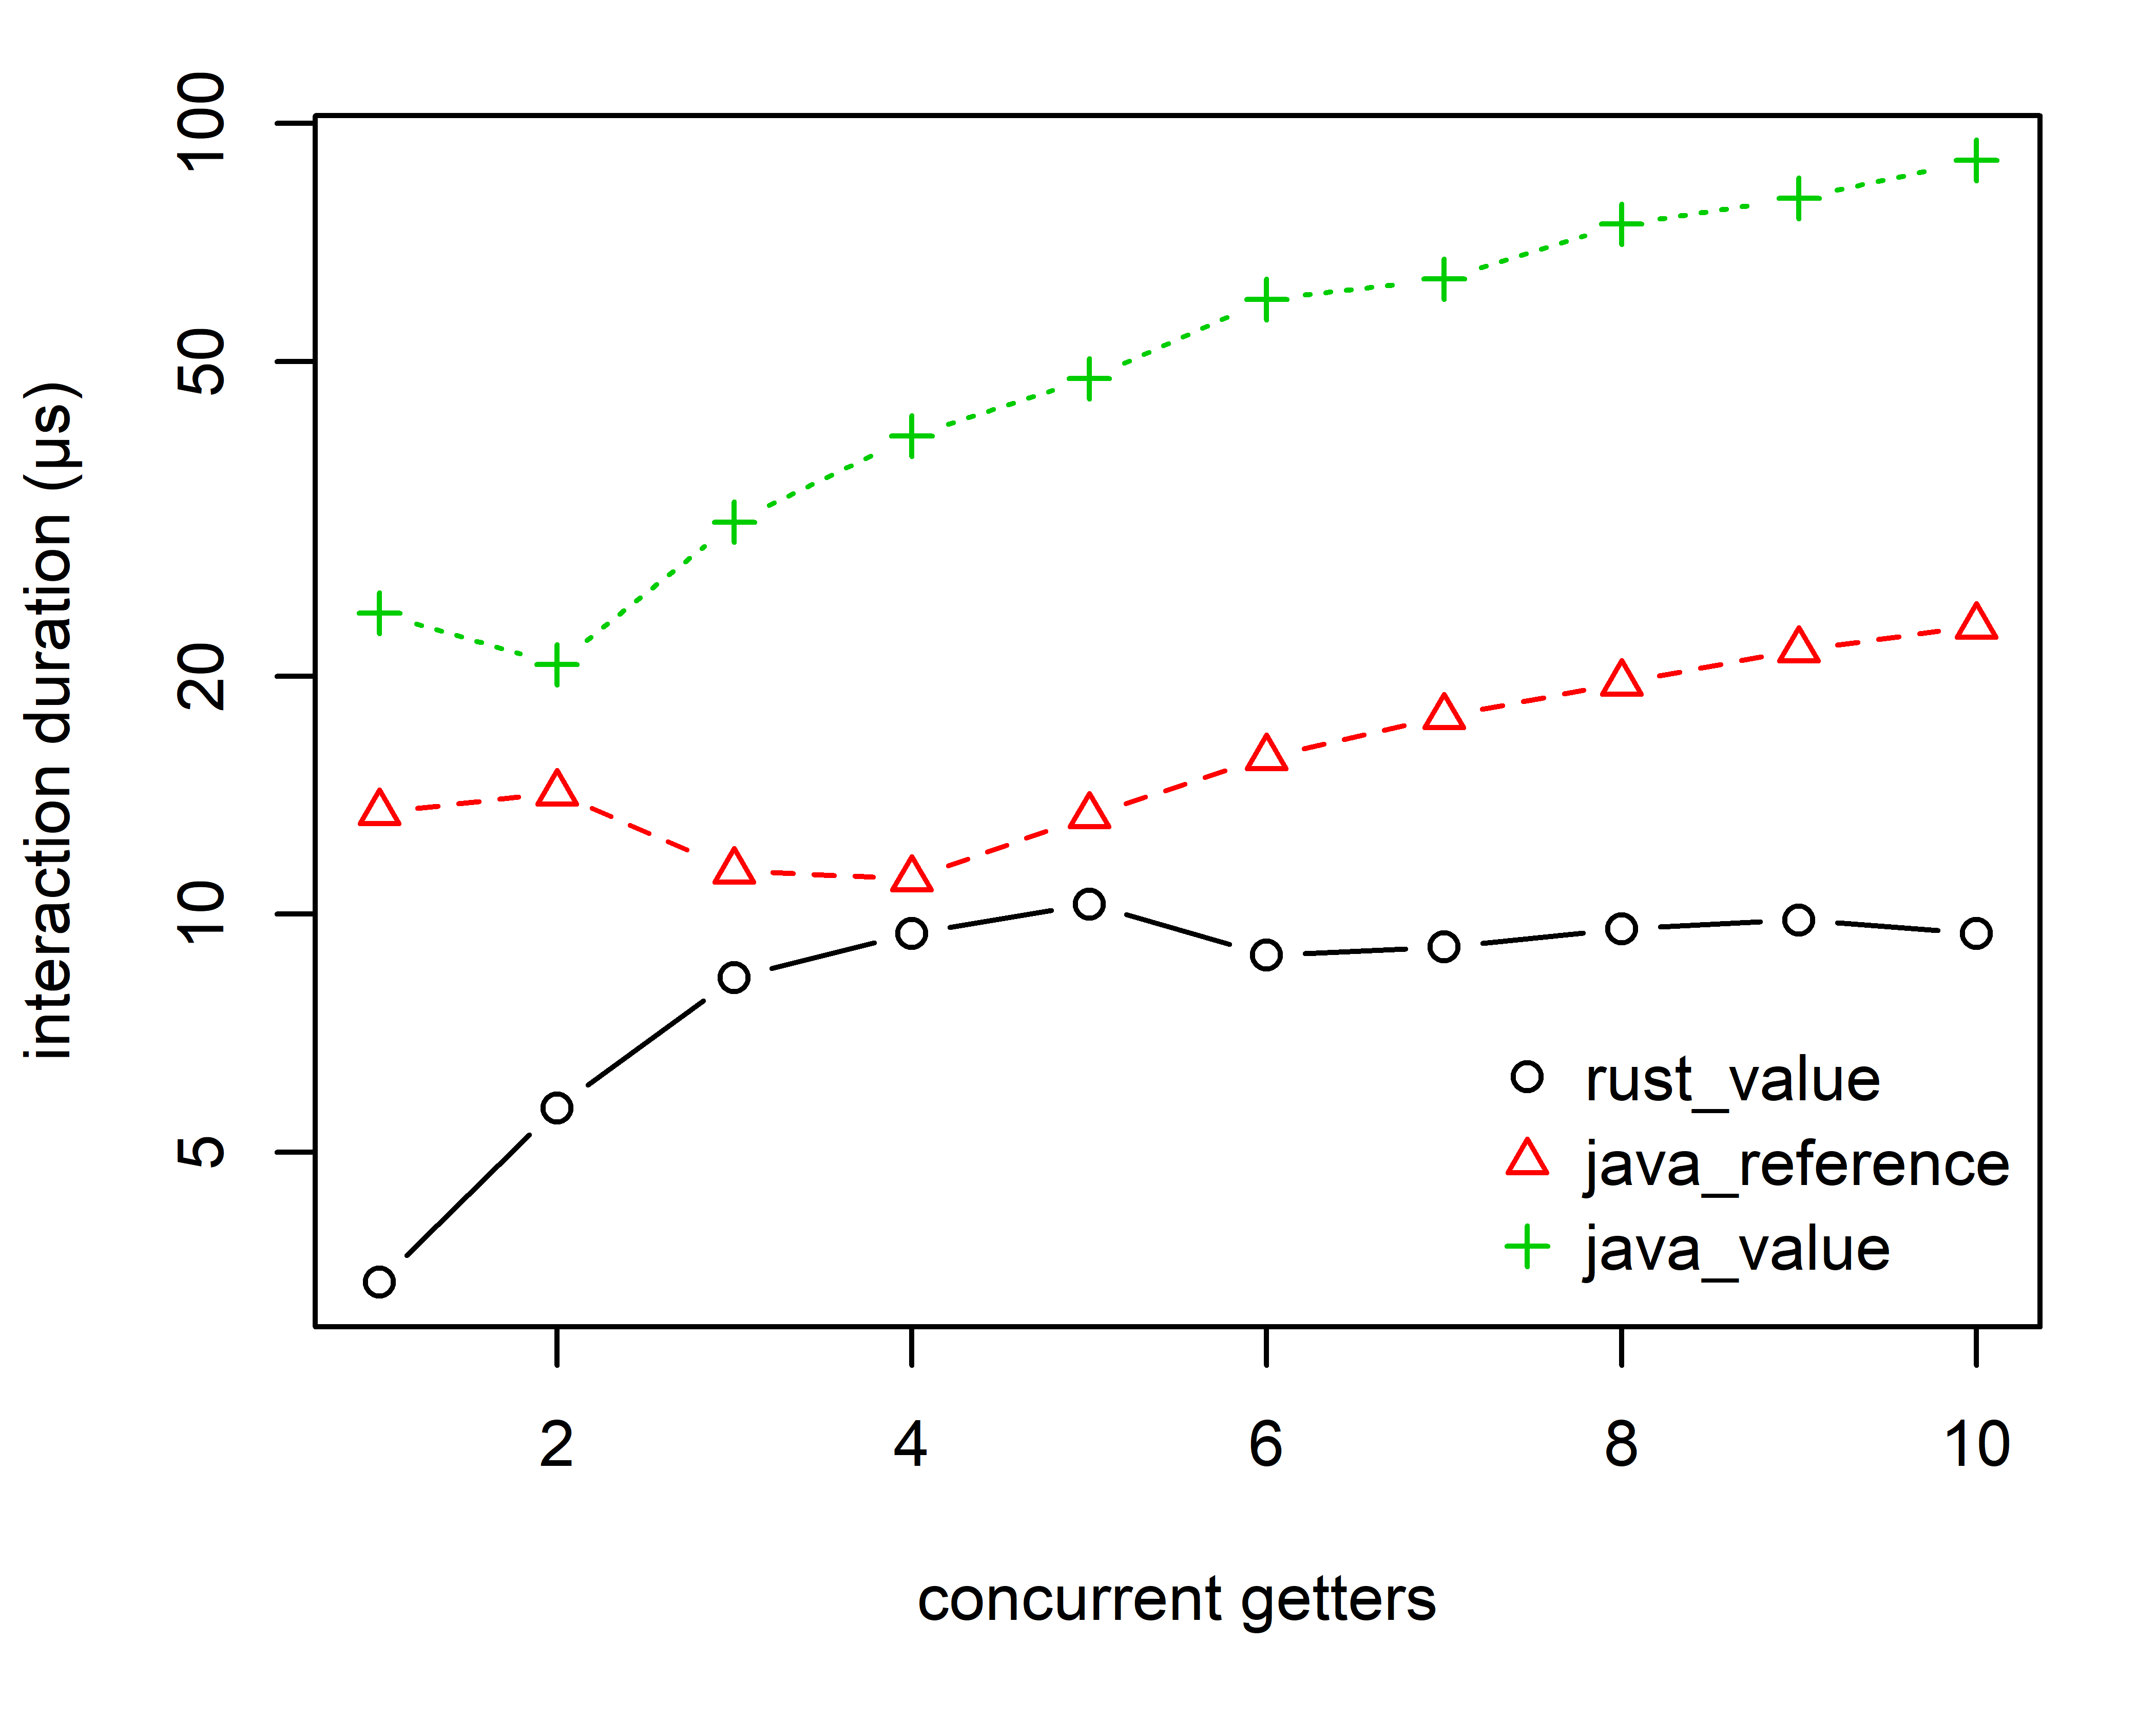
\includegraphics[width=0.80\textwidth]{experiments/rust_v_java_2.png}
	\caption[Java vs.\ Rust interaction time for large values.]{Comparison of interaction time for the \textit{fetch} connector for both Java and Rust backends moving 64-kilobyte-sized data. The Rust backend moves the datum by value, while the Java parallel `java\_reference' aliases the object (moving by reference). This backend does not support semantics-preserving value-passing. We achieve safety here by the coordinator injecting \code{clone} operations of byte arrays to mirror Rust's bit-wise copy, called `java\_value'. Note the logarithmic y-axis.}
	\label{fig:rust_v_java_2}
\end{figure}

\subsection{Versus Hand-Crafted Programs}

Clearly, Reo-rs cannot out-perform hand-optimized Rust on a case-by-case basis; whatever Reo-rs does, the hand-optimized code can mimic and specialize to surpass its performance. The utility of the library is to handle arbitrary Reo-generated protocol descriptions, hiding the details away from the user with an API that strikes a balance between flexibility, safety and performance. Here, we attempt to gauge the performance gap between Reo-rs for some small examples of connectors.

Firstly, we examine a case for which Reo-rs is expected to do poorly: the simple \textit{fifo1} connector. For this case, Reo-rs appears to overlook a myriad of optimization opportunities that are not available for connectors in general; for example, the port removing elements (the getter) wastes time checking if any other getters contend their removal of the buffered value (clearly not). Figure~\ref{fig:exper_rtt} compares the total `round trip time', measuring the mean duration of a `round trip' of a single element, ie.\ starting from the moment \code{put} begins to the moment \code{get} ends. Sub-figure~\ref{fig:exper_rtt_0} shows this in contrast to the simplest channels in Rust's standard library: \code{mpsc} (`multiple producer, single consumer').


\begin{figure}
	\centering
	\makebox[\textwidth][c]{
		\begin{subfigure}[b]{0.63\textwidth}
			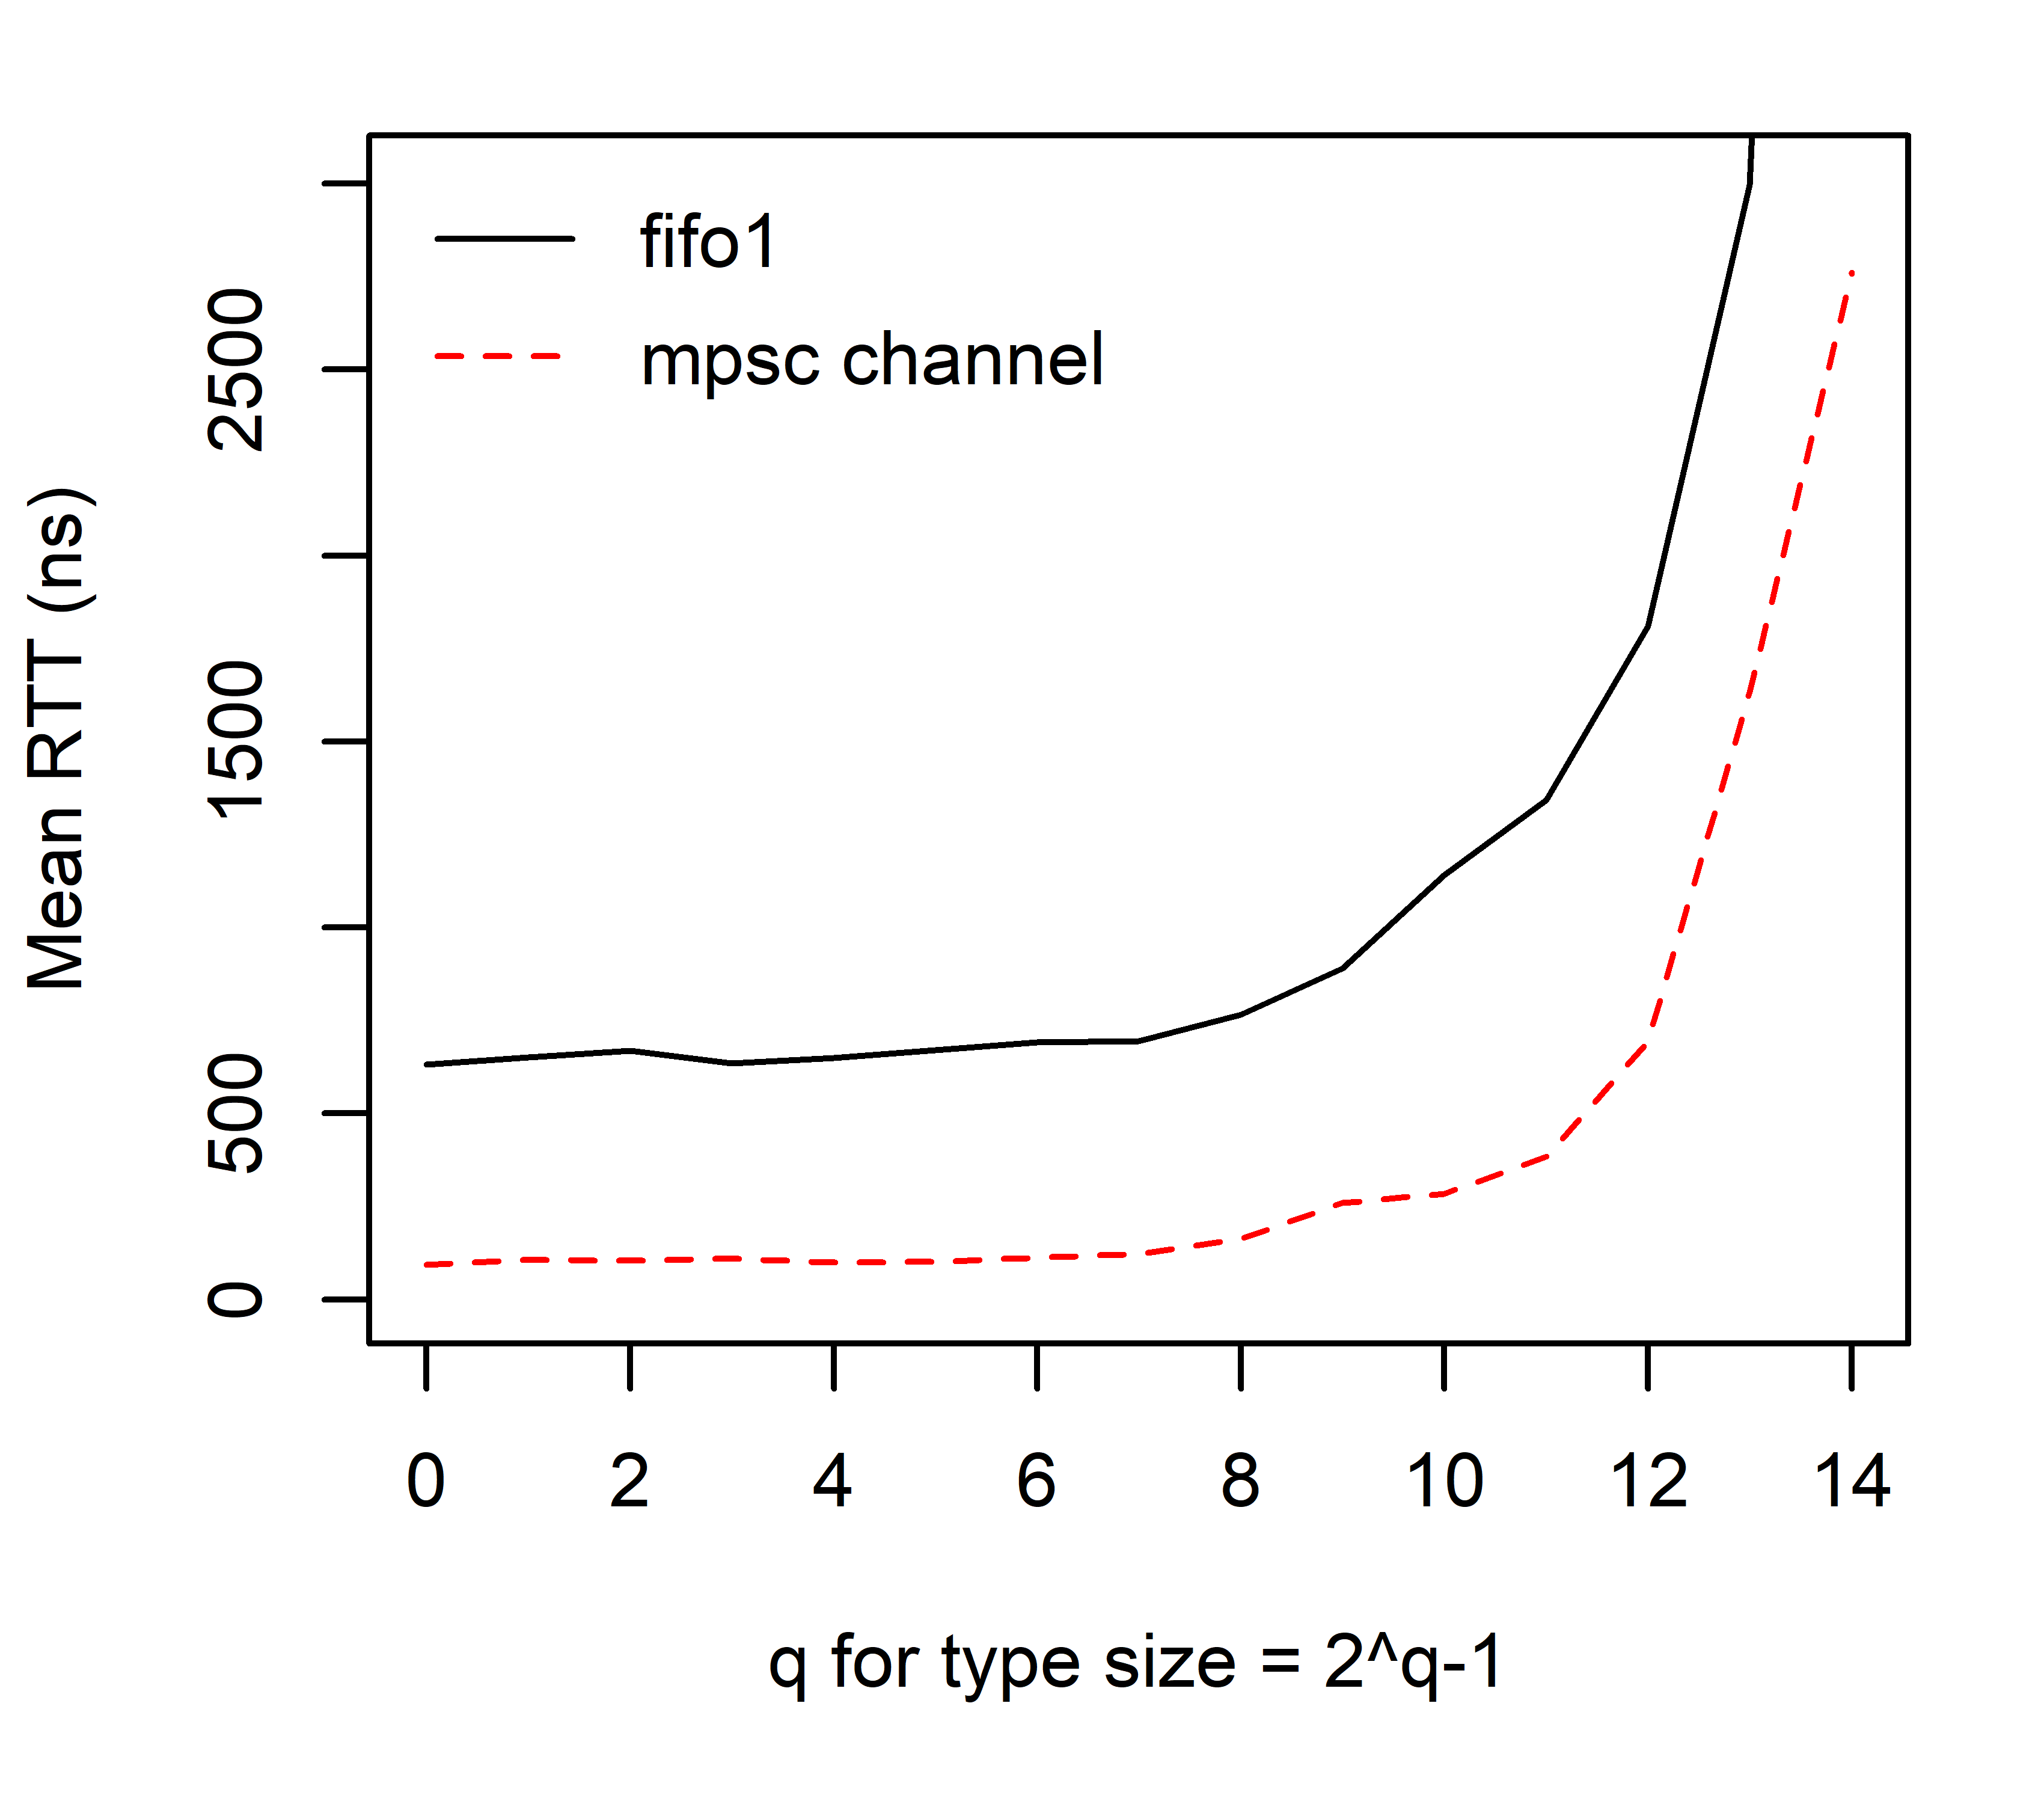
\includegraphics[width=\textwidth]{experiments/rtt_0.png}
			\caption{}
			\label{fig:exper_rtt_0}
		\end{subfigure}%
		\begin{subfigure}[b]{0.63\textwidth}
			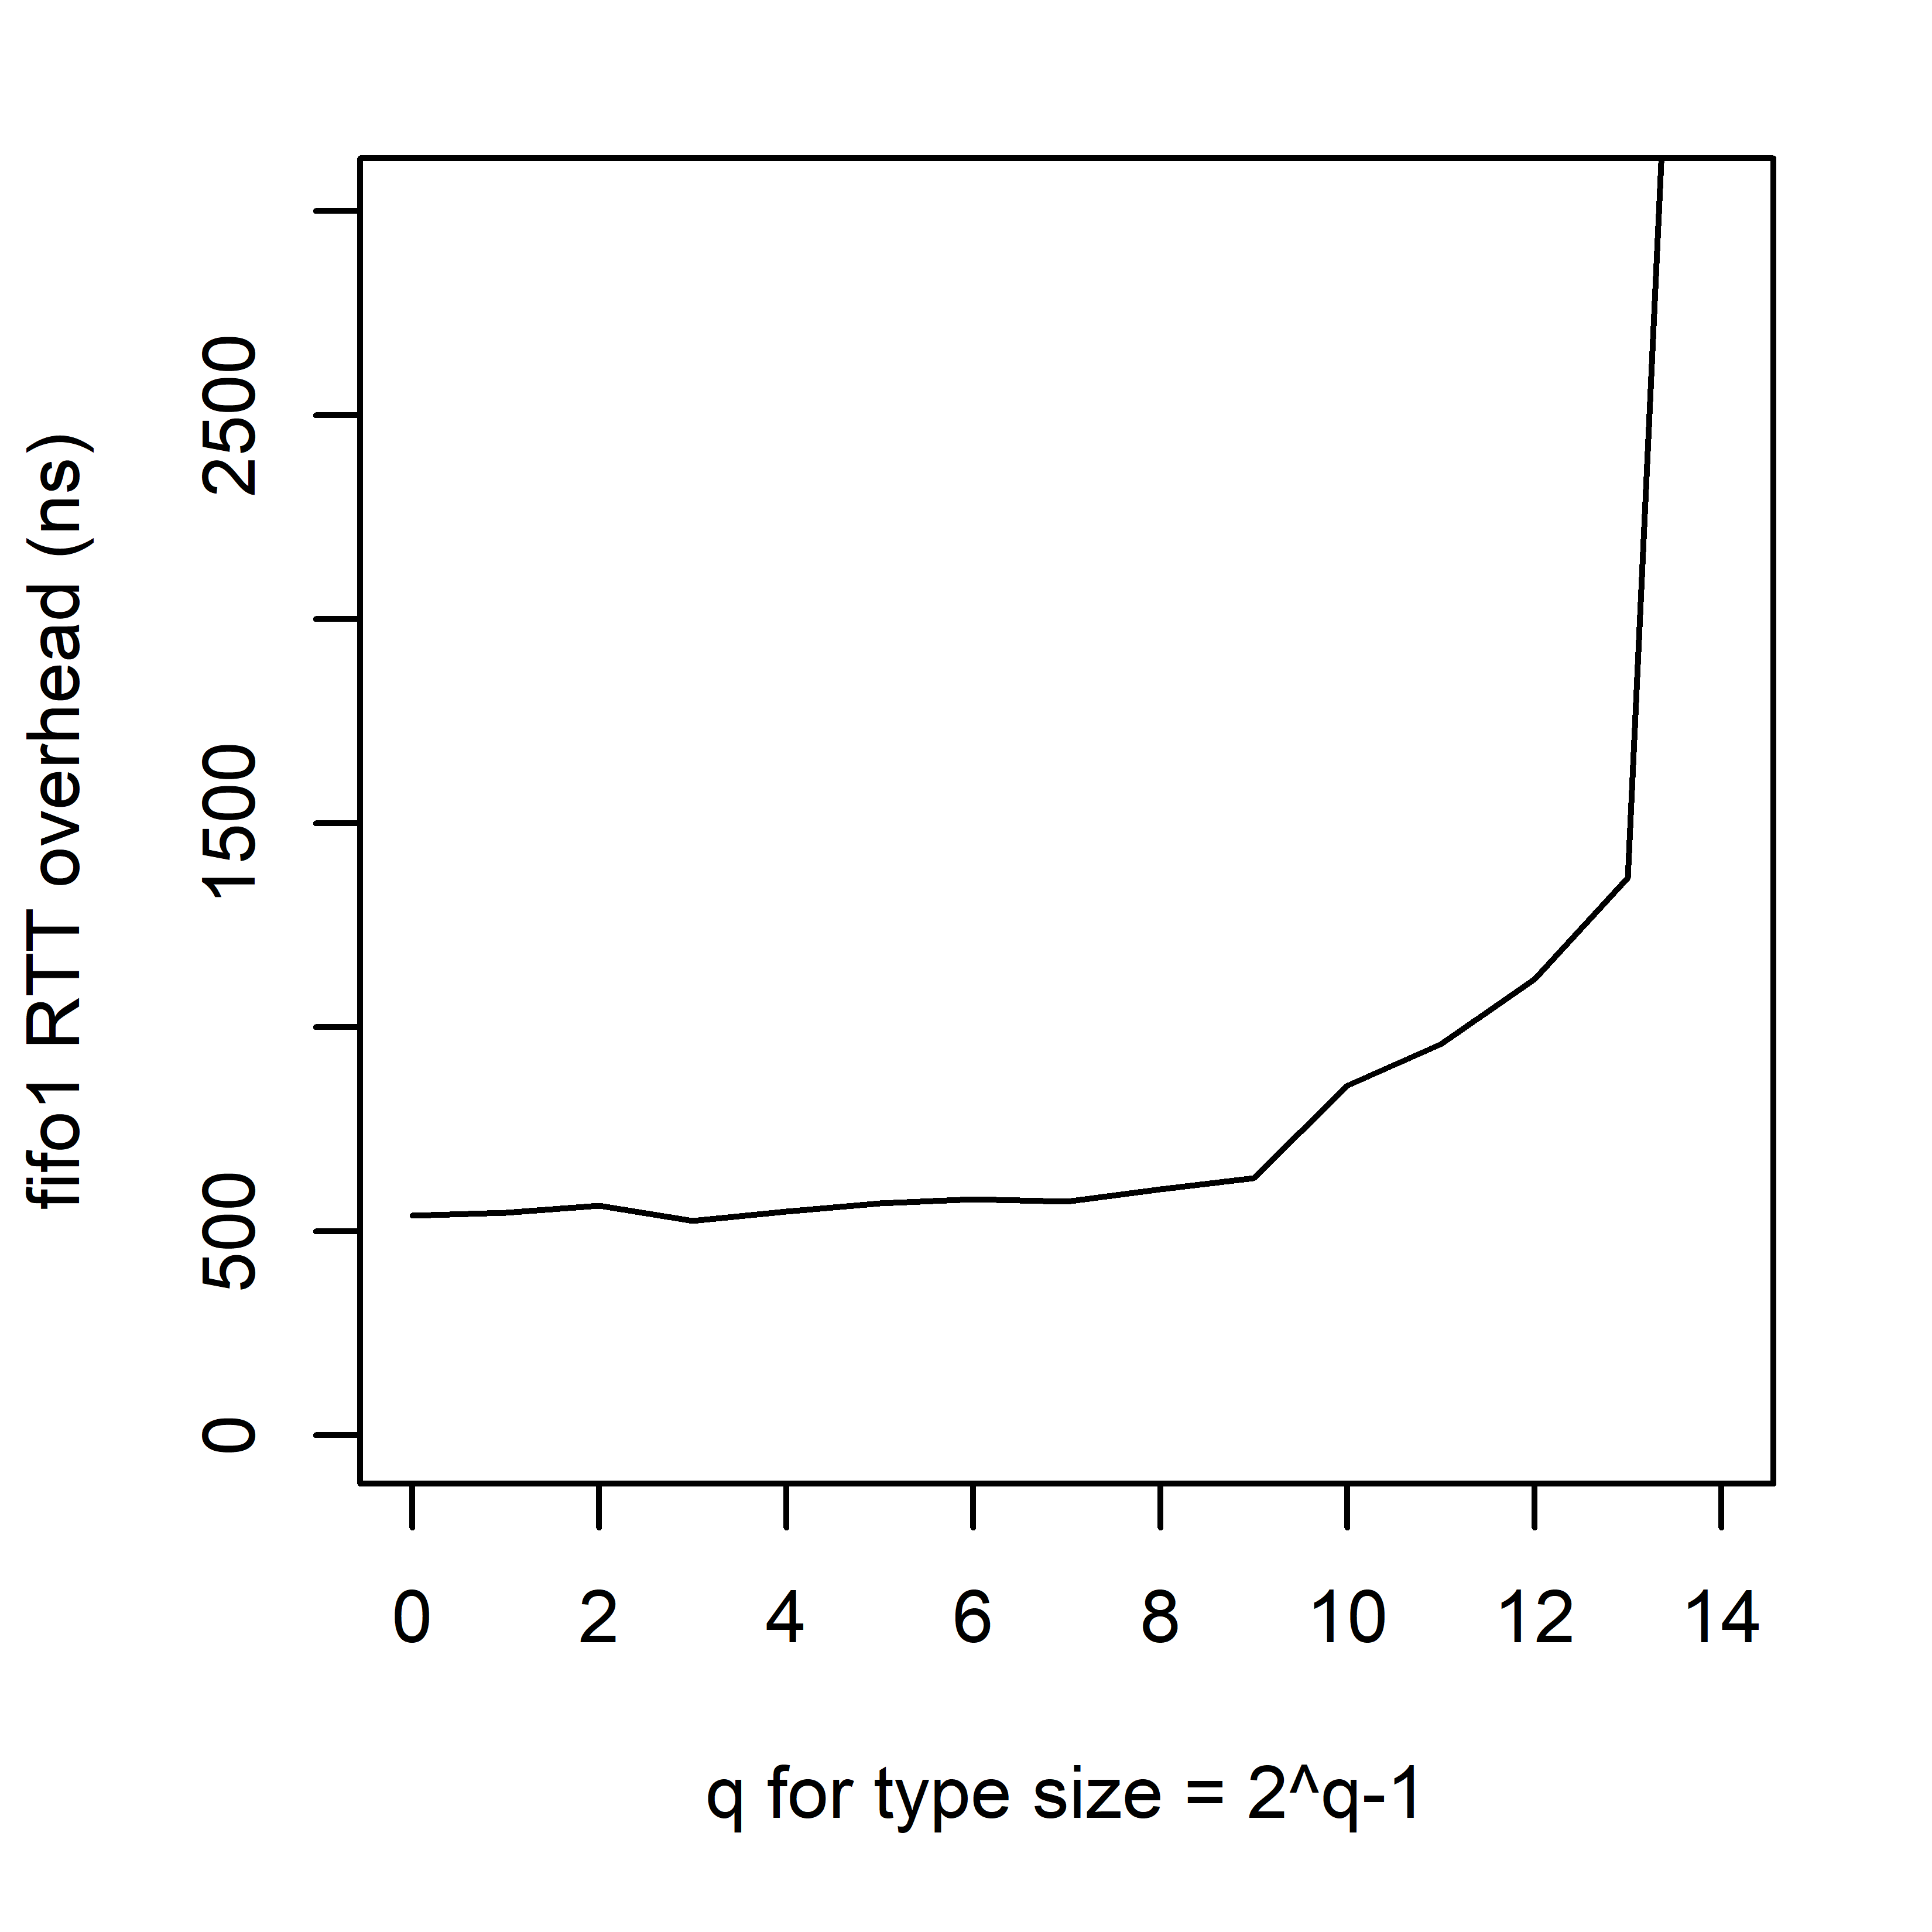
\includegraphics[width=\textwidth]{experiments/rtt_1.png}
			\caption{}
			\label{fig:exper_rtt_01}
		\end{subfigure}%
	}
	\caption[Performance of fifo1 connector vs.\ a standard channel type.]{Time from beginning of \code{put} to end of \code{get} in connector \textit{fifo1} compared to the time taken to send and received over an \code{mpsc} channel from the Rust standard library. Plots show the overhead in response to the size of the moved data. Figure~(b) shows the difference between the curves in Figure~(a), showing the overhead of Reo-rs more explicitly.}
	\label{fig:exper_rtt}
\end{figure}


These measurements show the range of times taken in response to changes in the data's size. The figure makes clear that compared to \code{mpsc}, Reo-rs experiences significant overhead in all cases. Some uniform overhead is to be expected, as \code{mpsc} is purpose-built and optimized for precisely this scenario. Reo-rs lacks the ability to optimize for this protocol to the same extent. For example, as explained in Section~\ref{sec:chosen_design}, all port-operations involve the acquisition of a shared protocol lock. Conceptually, Reo-rs has all the information it needs optimize for this protocol and particular and match the performance of \code{mpsc}. The generality of Reo-rs inhibits its ability to identify and specialize for these kinds of optimizations to the same extent as was done by hand for \code{mpsc}. A hand-optimized fifo1 channel could take advantage of the fact that the two ends of the channel need not share a lock at all. For this protocol, partitioning the coordinator such that each part only considers \textit{local} rules would be correct and cause less contention.

Figure~\ref{fig:exper_rtt_01} makes clear that Reo-rs is experiencing overhead that increases with the size of the moved value. At first glance, one can be forgiven for attributing this overhead to the presence of redundant movements of the data, which Section~\ref{sec:port_operations} explains can occur if llvm fails to optimize away the \textit{physical} movements from Rust's \textit{semantic} movements of values to new variable bindings. This turns out not to be the cause in this case. Rather, the overhead is caused by a more granular implementation detail; \code{mpsc} has a different method of moving its values. \code{mpsc} has some means to optimize data movements in the case of an x86-64 processor by `in-lining' it, spelling it out into a sequence of smaller movements hundreds of lines long. In this manner, \code{mpsc} is optimized to avoid the overhead of system calls\footnote{Listing~\ref{listing:mpsc_pop} in the Appendix gives a glimpse of the assembly for this procedure.}.


Things become more interesting when we apply Reo-rs to more complex problems that actually make use of its more expressive features such as synchrony and state. The \textit{alternator} is a canonical Reo circuit that routes messages from putters $\{P_0, P_1\}$ to getter $G$ in an alternating fashion (starting with $P_0$). The semantics of this connector are subtly different from that of a \textit{sequencer}; namely, the alternator only routes data when all three participants are simultaneously ready, after which $G$ receives a pair of messages in succession. The connector's semantics achieve this by transmitting the first value synchronously, and the dispatching latter asynchronously.
Listing~\ref{fig:alternator} shows an implementation of this protocol `by hand' in Rust using \code{Barrier} from the standard library, and the bounded-channel type from the ubiquitous \code{crossbeam} library with bounds~0 and~1 to act as synchronous (\textsc{aka} rendezvous) and asynchronous (\textsc{aka} buffered) channels for data. Figure~\ref{fig:alternator} shows the experimental results. Reo-rs never out-performed the hand-crafted code, but it was never far behind. As seen before, these optimized channels are able to more efficiently move data by using in-lining optimizations, increasing the gap as data gets larger. For values large enough to benefit from it, the figure also shows the speedup achieved by using the \textit{unsafe} reference-passing API, described in Section~\ref{sec:port_operations}.

Reo-rs is designed to handle the expressivity that characterizes the Reo language. The more synchronous and stateful a connector becomes, the more Reo-rs-\textit{like} the handcrafted implementation will be.

\begin{figure}
	\centering
	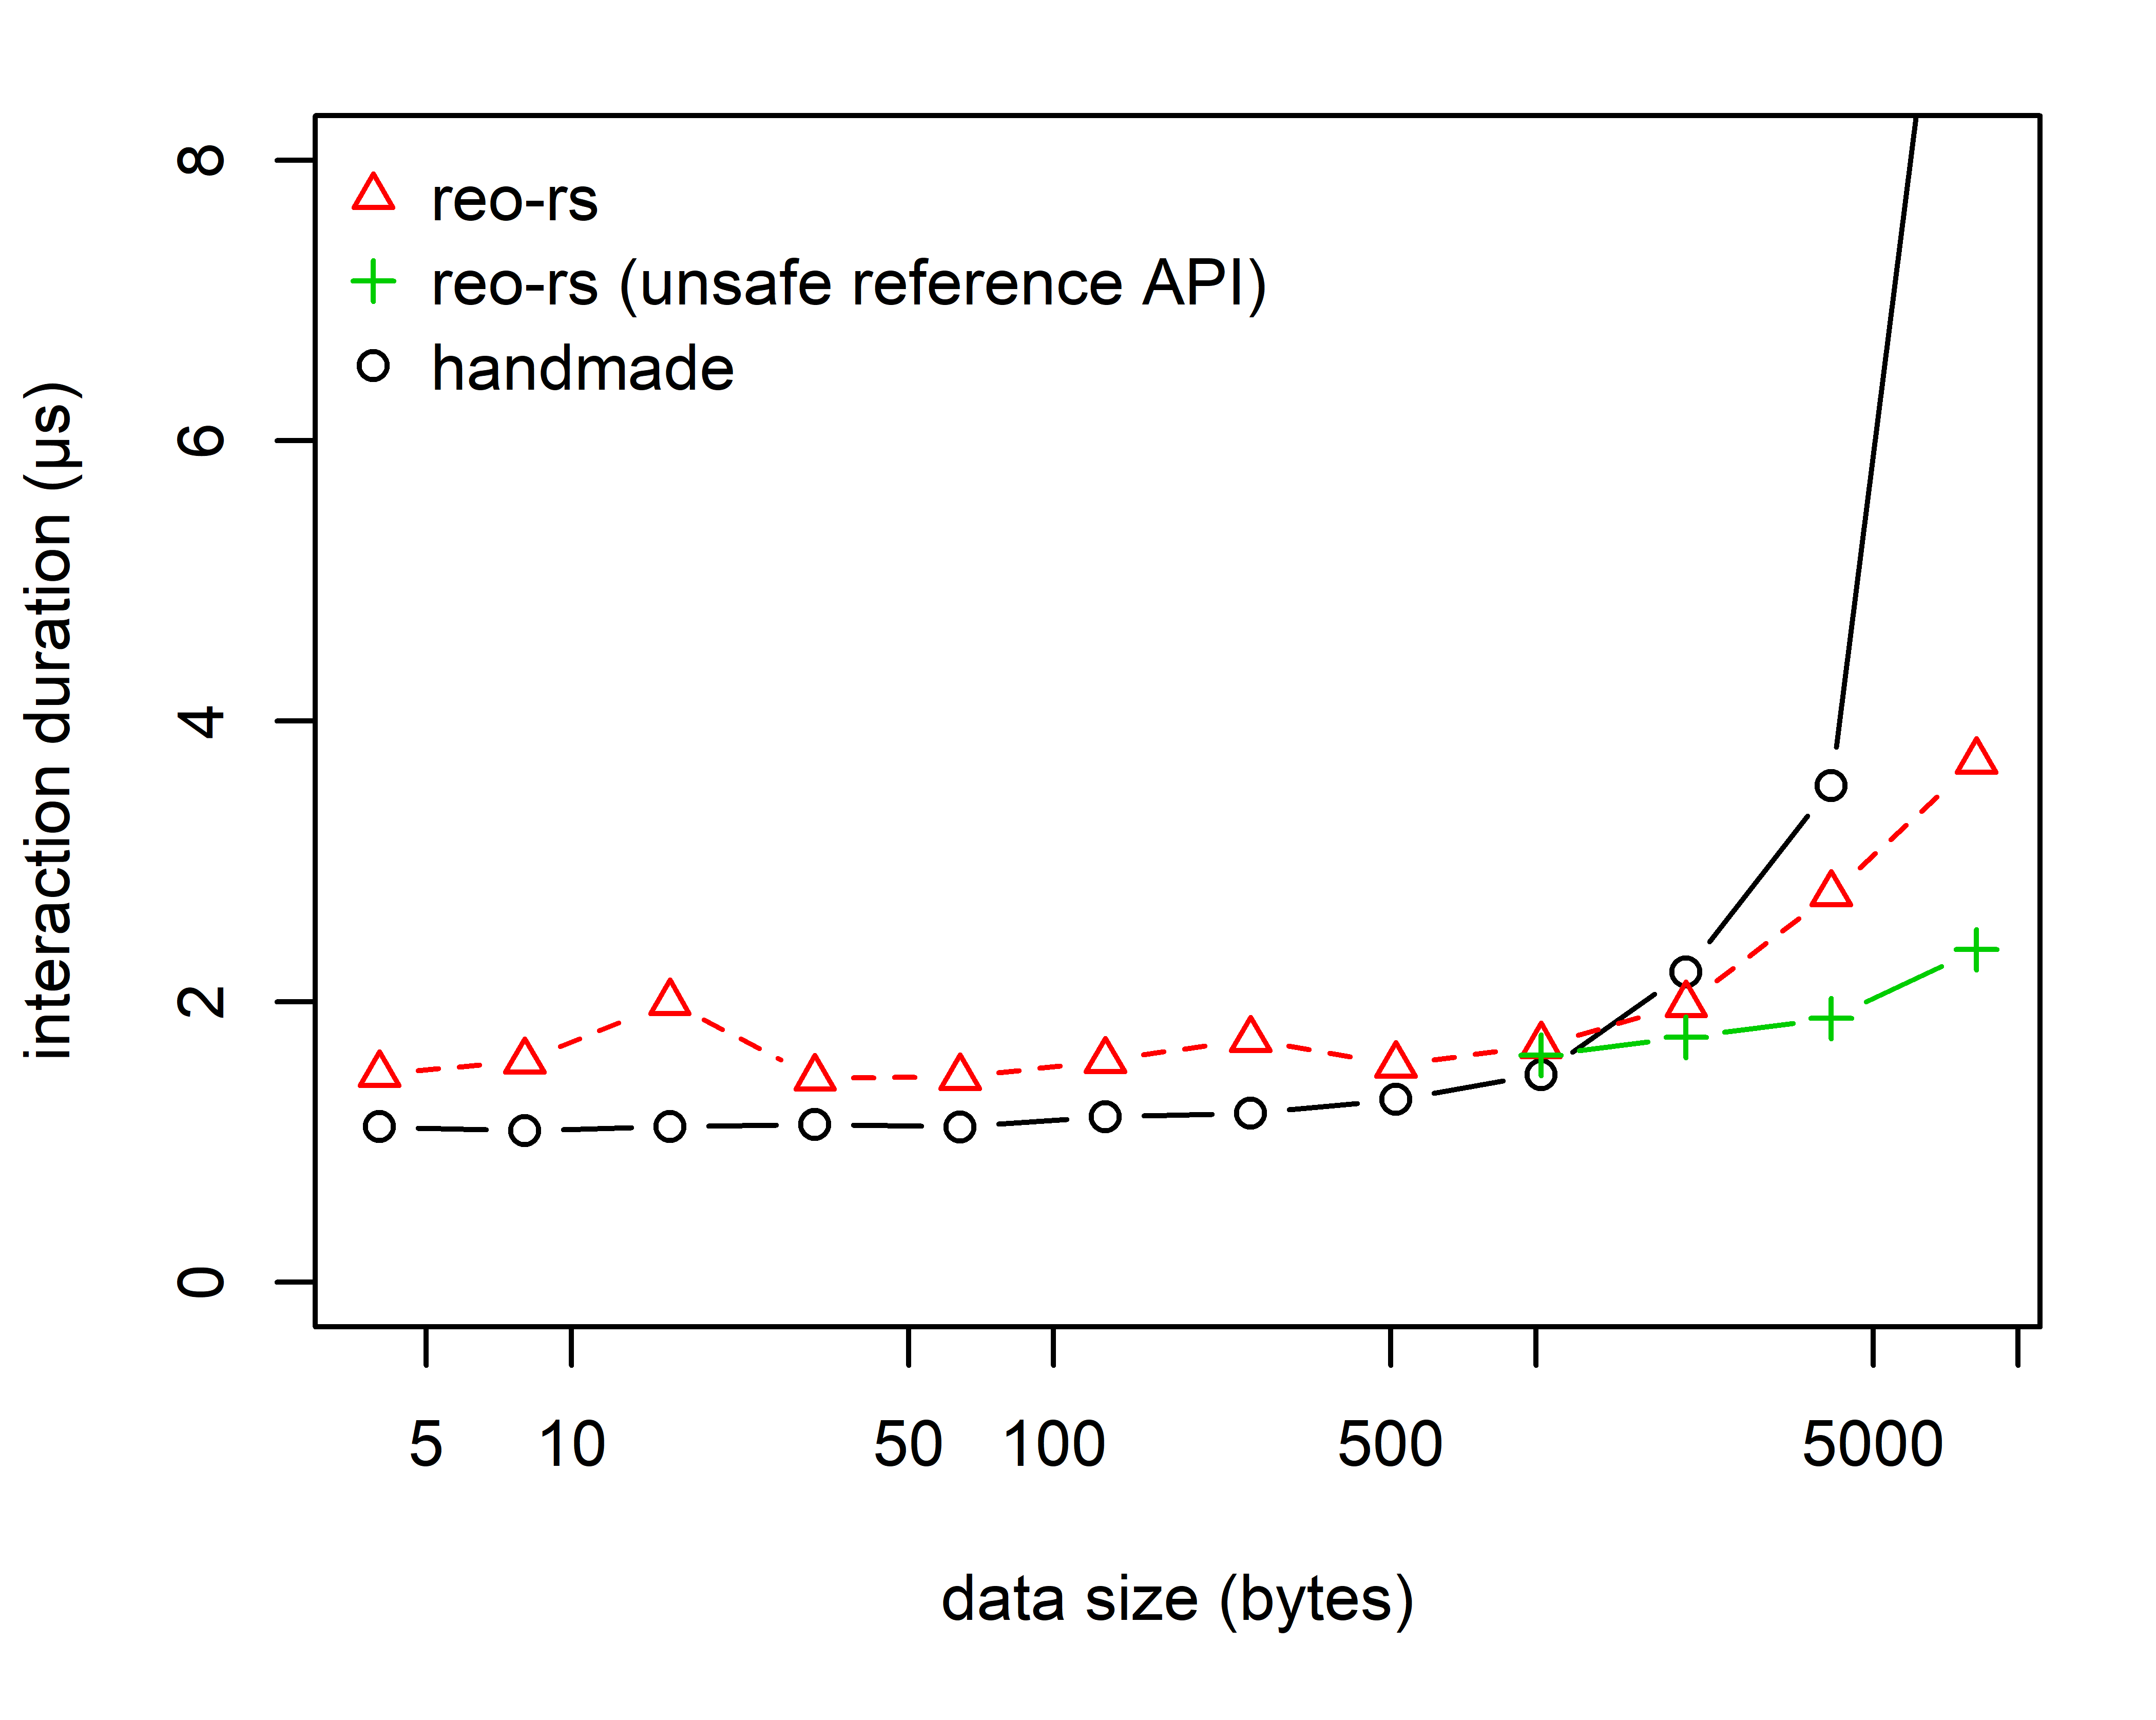
\includegraphics[width=0.80\textwidth]{experiments/alternator.png}
	\caption[Hand-crafted vs.\ Reo-generated Alternator.]{TODO.}
	\label{fig:alternator}
\end{figure}

\section{Overhead Examined}
Here, we examine the performance characteristics of Reo-rs in more detail under various circumstances. The goal is to understand how Reo-rs uses its computational resources, and how performance responds to properties of the specific protocol.

\subsection{Port-Operation Parallelism}

For connectors as simple as \textit{fifo1}, overhead is overhead. However, we are particularly interested in understanding how this overhead is partitioned; as connectors become more complex, different parts of this overhead impact \textit{parallelism} in different ways. Section~\ref{sec:protocol_runtime} explains the nature of the \textit{coordinator} role, and how its operations are performed holding the lock for the \code{Proto} instance which connects ports as their common communication medium. Table~\ref{tab:active_time} shows measurements for an experiment that attempts to understand which proportion of our overhead is incurred \textit{inside} the critical region, ie.\ by the coordinator. In the case of this experiment, our protocol has rules for movement which can be rendered as a \textit{bipartite graph}, allowing data flow from any putter in $\{P0, P1, P2\}$ to any getter in $\{G0, G1, G2\}$. As explained in Section~\ref{sec:data_exchange}, movements such as these do not buffer the data elements inside the protocol; getters take values from putters directly. As a consequence, putters are both the first and last to parttake in any of our rule firings' data movements. The table shows the mean duration for which each putter was involved in such a firing. Along with the total duration of the run, we are able to compute to which extent these putters were able to work in parallel. We distinguish between four cases, corresponding to rows in Table~\ref{tab:active_time}. The first three cases do not involve the \code{clone} operation, and are observed to have insignificant differences for all measurements. For this experiment, with modestly-sized values, we conclude that there is no large difference in performance between these three cases:
\begin{enumerate}
	\item [\textbf{move}] Values are moved from putter to getter synchonously.
	\item [\textbf{copy}] Putters retain their values, and getters replicate them with a bit-wise copy that does not mutate the original.
	\item [\textbf{signal}] Getters do not return any data. They return after releasing putters.
\end{enumerate}

The final \textbf{clone} case attempts to observe the effects of intentionally delaying getters outside of the lock by necessitating the use of an explicit \code{clone} operation whose duration is artificially lengthened\footnote{\code{sleep} calls were out of the question, as its variability is overwhelming at this scale. Instead, \code{clone} perform thousands of chaotic integer computations on the replica before returning it. This is intentionally obtuse such that the Rust compiler is unable to identify a trivializing optimization.}. For these runs, putters retained their original values, but the datum was not marked with the \code{Copy} trait. In all cases, we observed that even at this coarse granularity, there was significant parallelism. For the majority of the time, new rules were able to fire whilst interactions were being completed outside of the critical region. The final case in particular was within a small rounding error of perfect parallelism.

\begin{table}[]
	\begin{tabular}{l|lll|ll}
		& \multicolumn{3}{l|}{mean active time} & \multirow{2}{*}{\begin{tabular}[c]{@{}l@{}}run\\ duration\end{tabular}} & \multirow{2}{*}{\begin{tabular}[c]{@{}l@{}}mean\\ parallelism\end{tabular}} \\
		& p0 & p1 & p2 &  &  \\ \hline
		move & 2.037µs, & 2.031µs, & 2.017µs & 214.991ms & 2.83 \\
		copy & 1.744µs, & 1.852µs, & 1.844µs & 197.676ms & 2.75 \\
		signal & 1.962µs, & 1.956µs, & 1.937µs & 207.181ms & 2.83 \\
		\hline
		clone & 94.021µs, & 94.082µs, & 94.058µs & 9420.148ms & 2.995 
	\end{tabular}
	\caption[Parallelism between getters in runs of the SISO connector.]{Runs of 3 putters greedily sending their data directly to any of 3 getters, 100000 times. This test was performed with 4~variants, differing on the properties of the data and whether the putter retained the original. The last column is derived, showing to what extent these putters were able to work in parallel.}
	\label{tab:active_time}
\end{table}

\subsection{Overhead Inside the Critical Region}
The previous section, we saw an experiment with data moving between putters and getters. These runtimes included the putter's time spent not only on the movement itself, but also on the time spent in the role of \textit{coordinator}. Here, we examine the work that pertains to this role and how changes to the definition of rules influence overhead. Figure~\ref{fig:check_time} shows the overhead incurred by a coordinator that traverses \textit{unsatisfied} rules before finding one to fire. It is apparent that in all cases, the overhead scales linearly, as expected. The time taken to evaluate the satisfaction of a rule varies greatly dependent on its definition; the evaluation of a rule involves many different operations mirroring the intricacies of the \textit{imperative form} it models, described in Chapter~\ref{sec:imperative_form}. To represent the possibility space, the figure shows measurements for a simple protocol which encounters replicas of one unsatisfied rule repeatedly, where its nature comes in four distinct variants:
\begin{enumerate}
	\item [\textbf{guard}] A rule where some port is not ready. This is detected almost immediately by cheap \textit{bit vector} operations, as explained in Section~\ref{sec:minimizing_the_bottleneck}. Evaluation takes 8.76ns.
	
	\item [\textbf{false}] A rule whose first instruction checks the predicate \textit{false}. Evaluation takes 18.91ns.
	\item [\textbf{ands}] A rule whose first instruction is a tree-like formula structure of twenty-five conjunctions, only the last of which is \textit{false}. Evaluation takes 180.72ns.
	\item [\textbf{alloc}] A rule whose first instruction allocates a fresh boolean-type resource with value \textit{false}. The second instruction checks that this temporary value is true. Upon failure, the allocation must be rolled back, discarding the temporary value. Evaluation takes 316.51ns.
\end{enumerate}


\begin{figure}
	\centering
	\makebox[\textwidth][c]{
		\begin{subfigure}[b]{0.63\textwidth}
			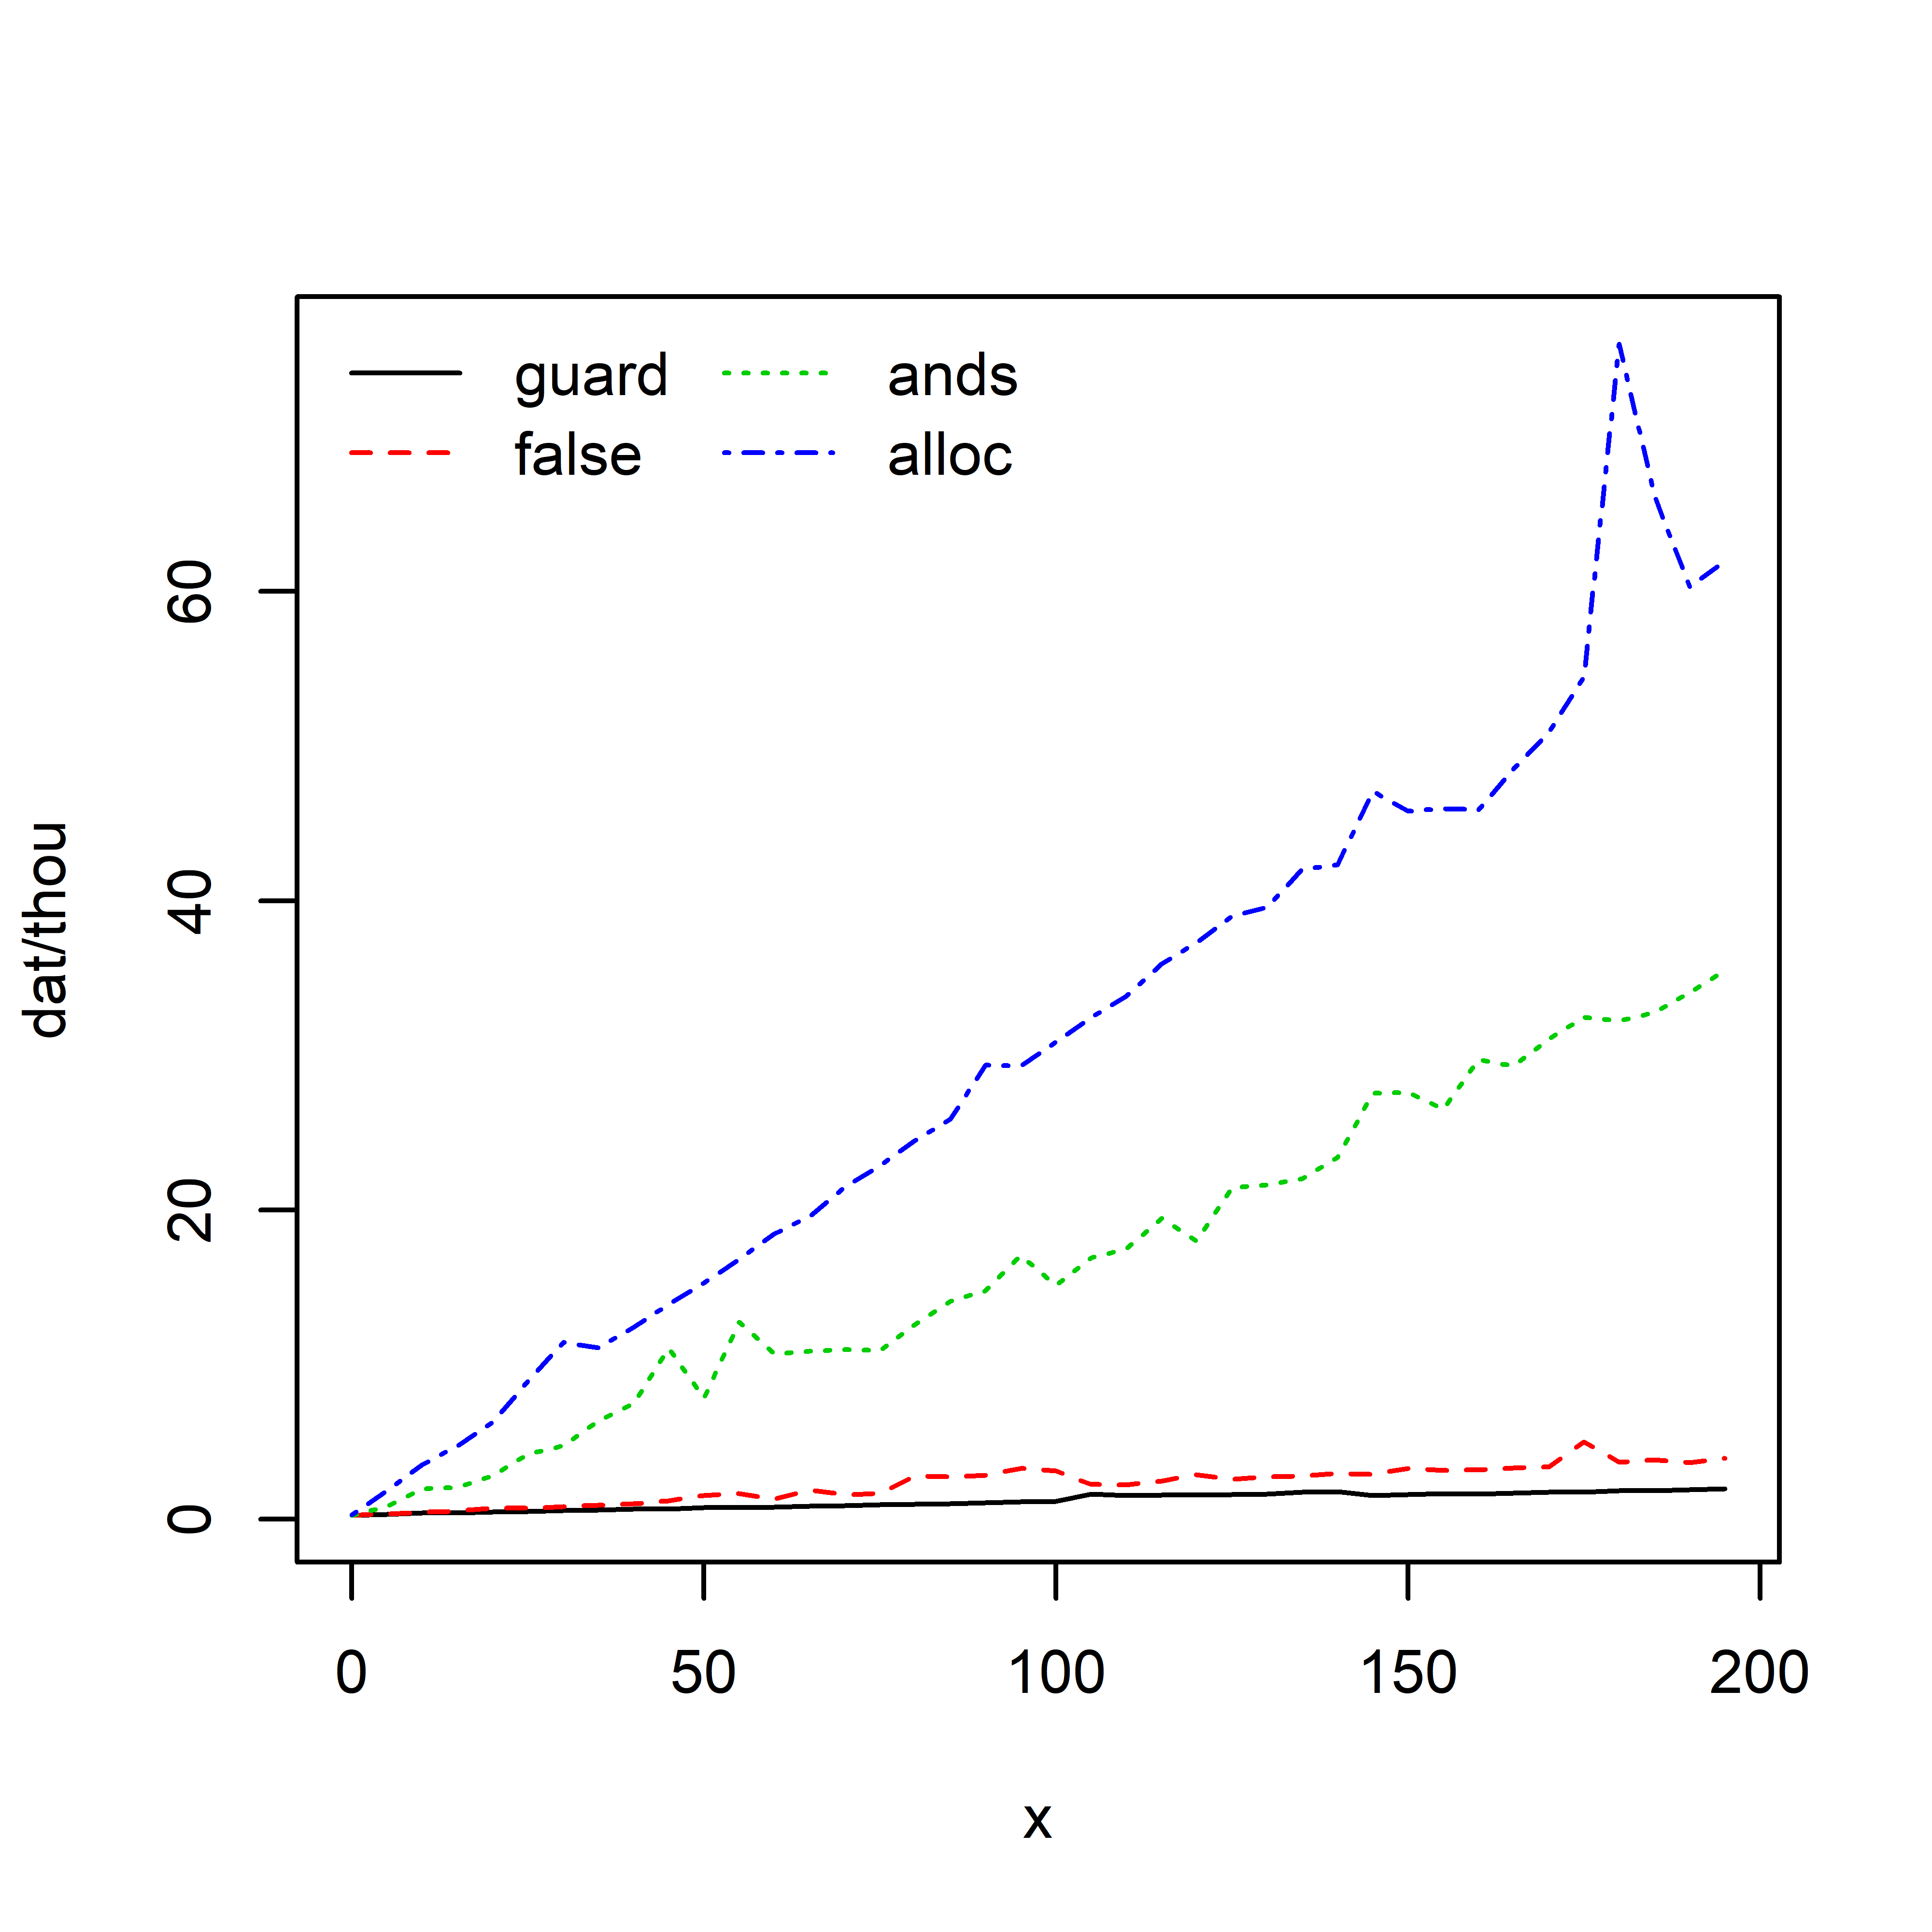
\includegraphics[width=\textwidth]{experiments/check_time_0.png}
			\caption{}
			\label{fig:check_time_0}
		\end{subfigure}%
		\begin{subfigure}[b]{0.63\textwidth}
			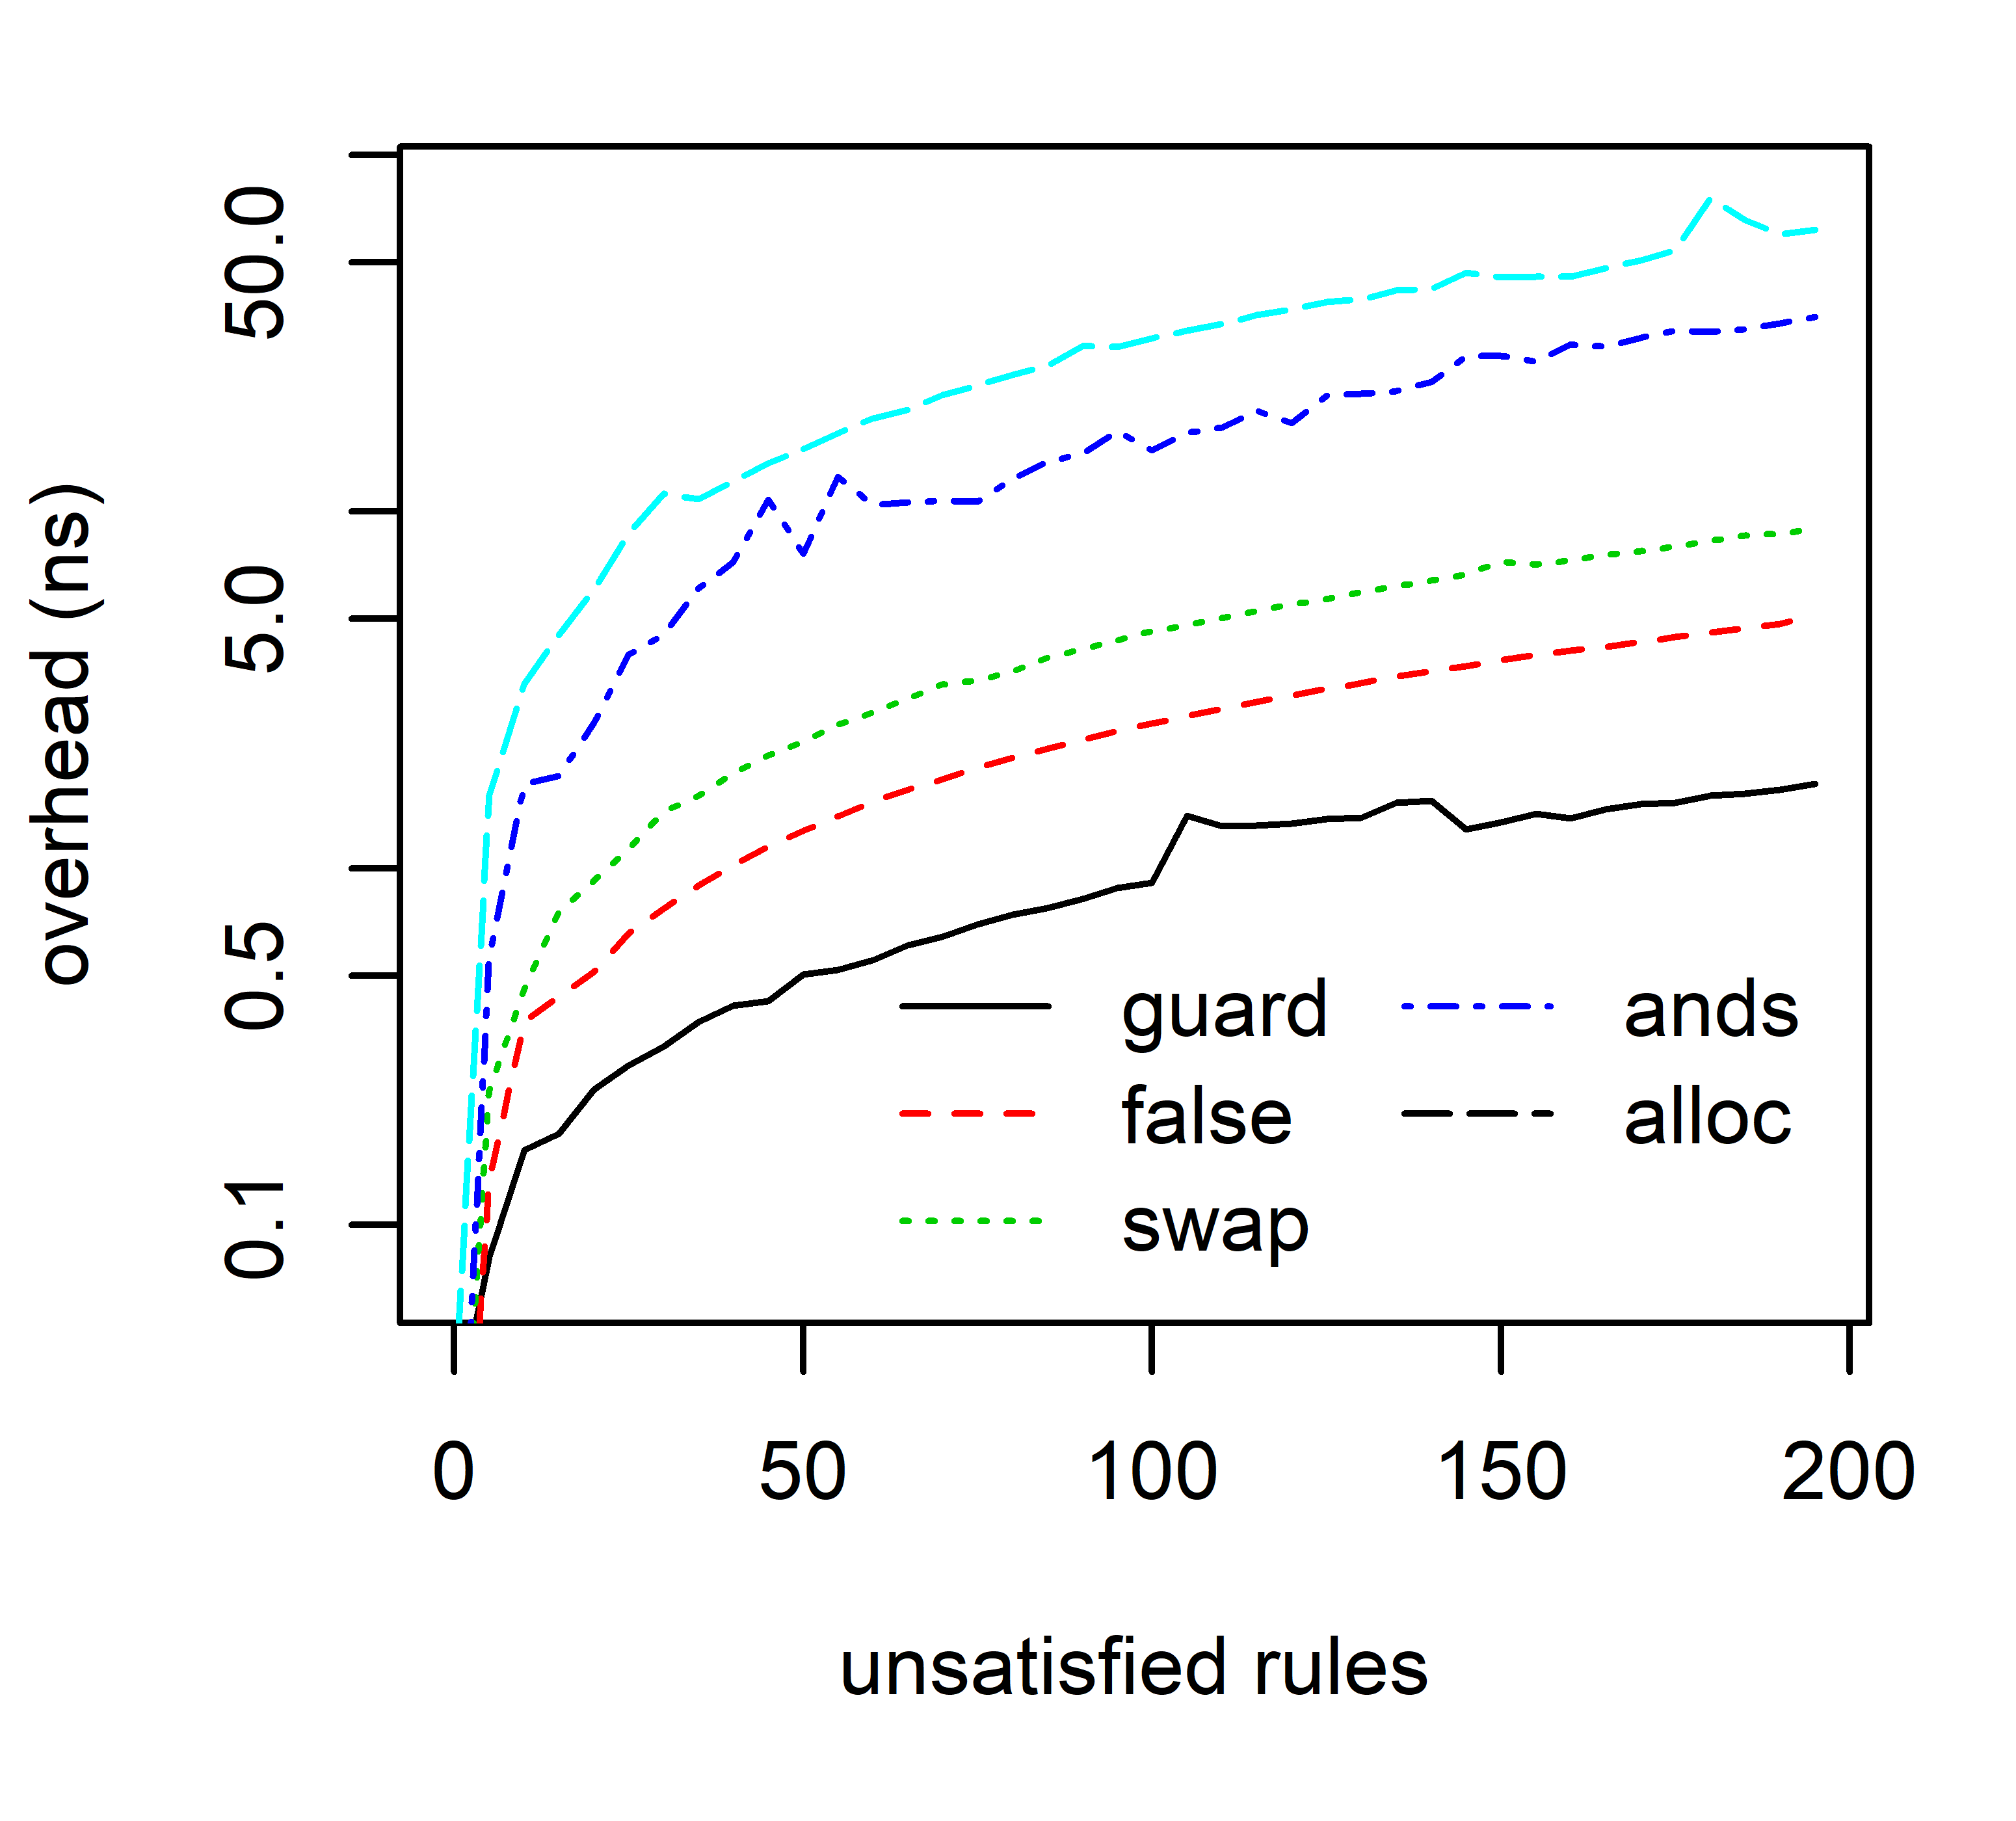
\includegraphics[width=\textwidth]{experiments/check_time_1.png}
			\caption{}
			\label{fig:check_time_2}
		\end{subfigure}%
	}
	\caption[Overhead of evaluating unsatisfied rules.]{Overhead as a result of evaluating a sequence of identical unsatisfied rules before firing something. Experiment is repeated for four variants of unsatisfied rules varying in the complexity of the operations they before before being deemed unsatisfied. The two sub-figures show the same information, with (b) representing it with a logarithmic y-axis to accentuate the small-scale differences.}
	\label{fig:check_time}
\end{figure}

These results meet our expectations. Rules can be arbitrarily complex, and perform an arbitrary amount of work before concluding that they are not satisfied, and will not fire. Even for this small set of relatively simple examples, we are able to see orders of magnitude in difference between the best case (in which the rule is skipped as early as possible by evaluating a bit-vector), to the worst case (involving several complex instructions). Fortunately, realistic Reo connectors will be defined almost entirely by rules that are either skipped as a result of evaluating these bit-vectors, or not at all. Even more expensive guards can expect to incur overhead in the order of nanoseconds as long as they involve no more than a handful of reasonable instructions. 

\begin{figure}
	\centering
	\makebox[\textwidth][c]{
		\begin{subfigure}[b]{0.63\textwidth}
			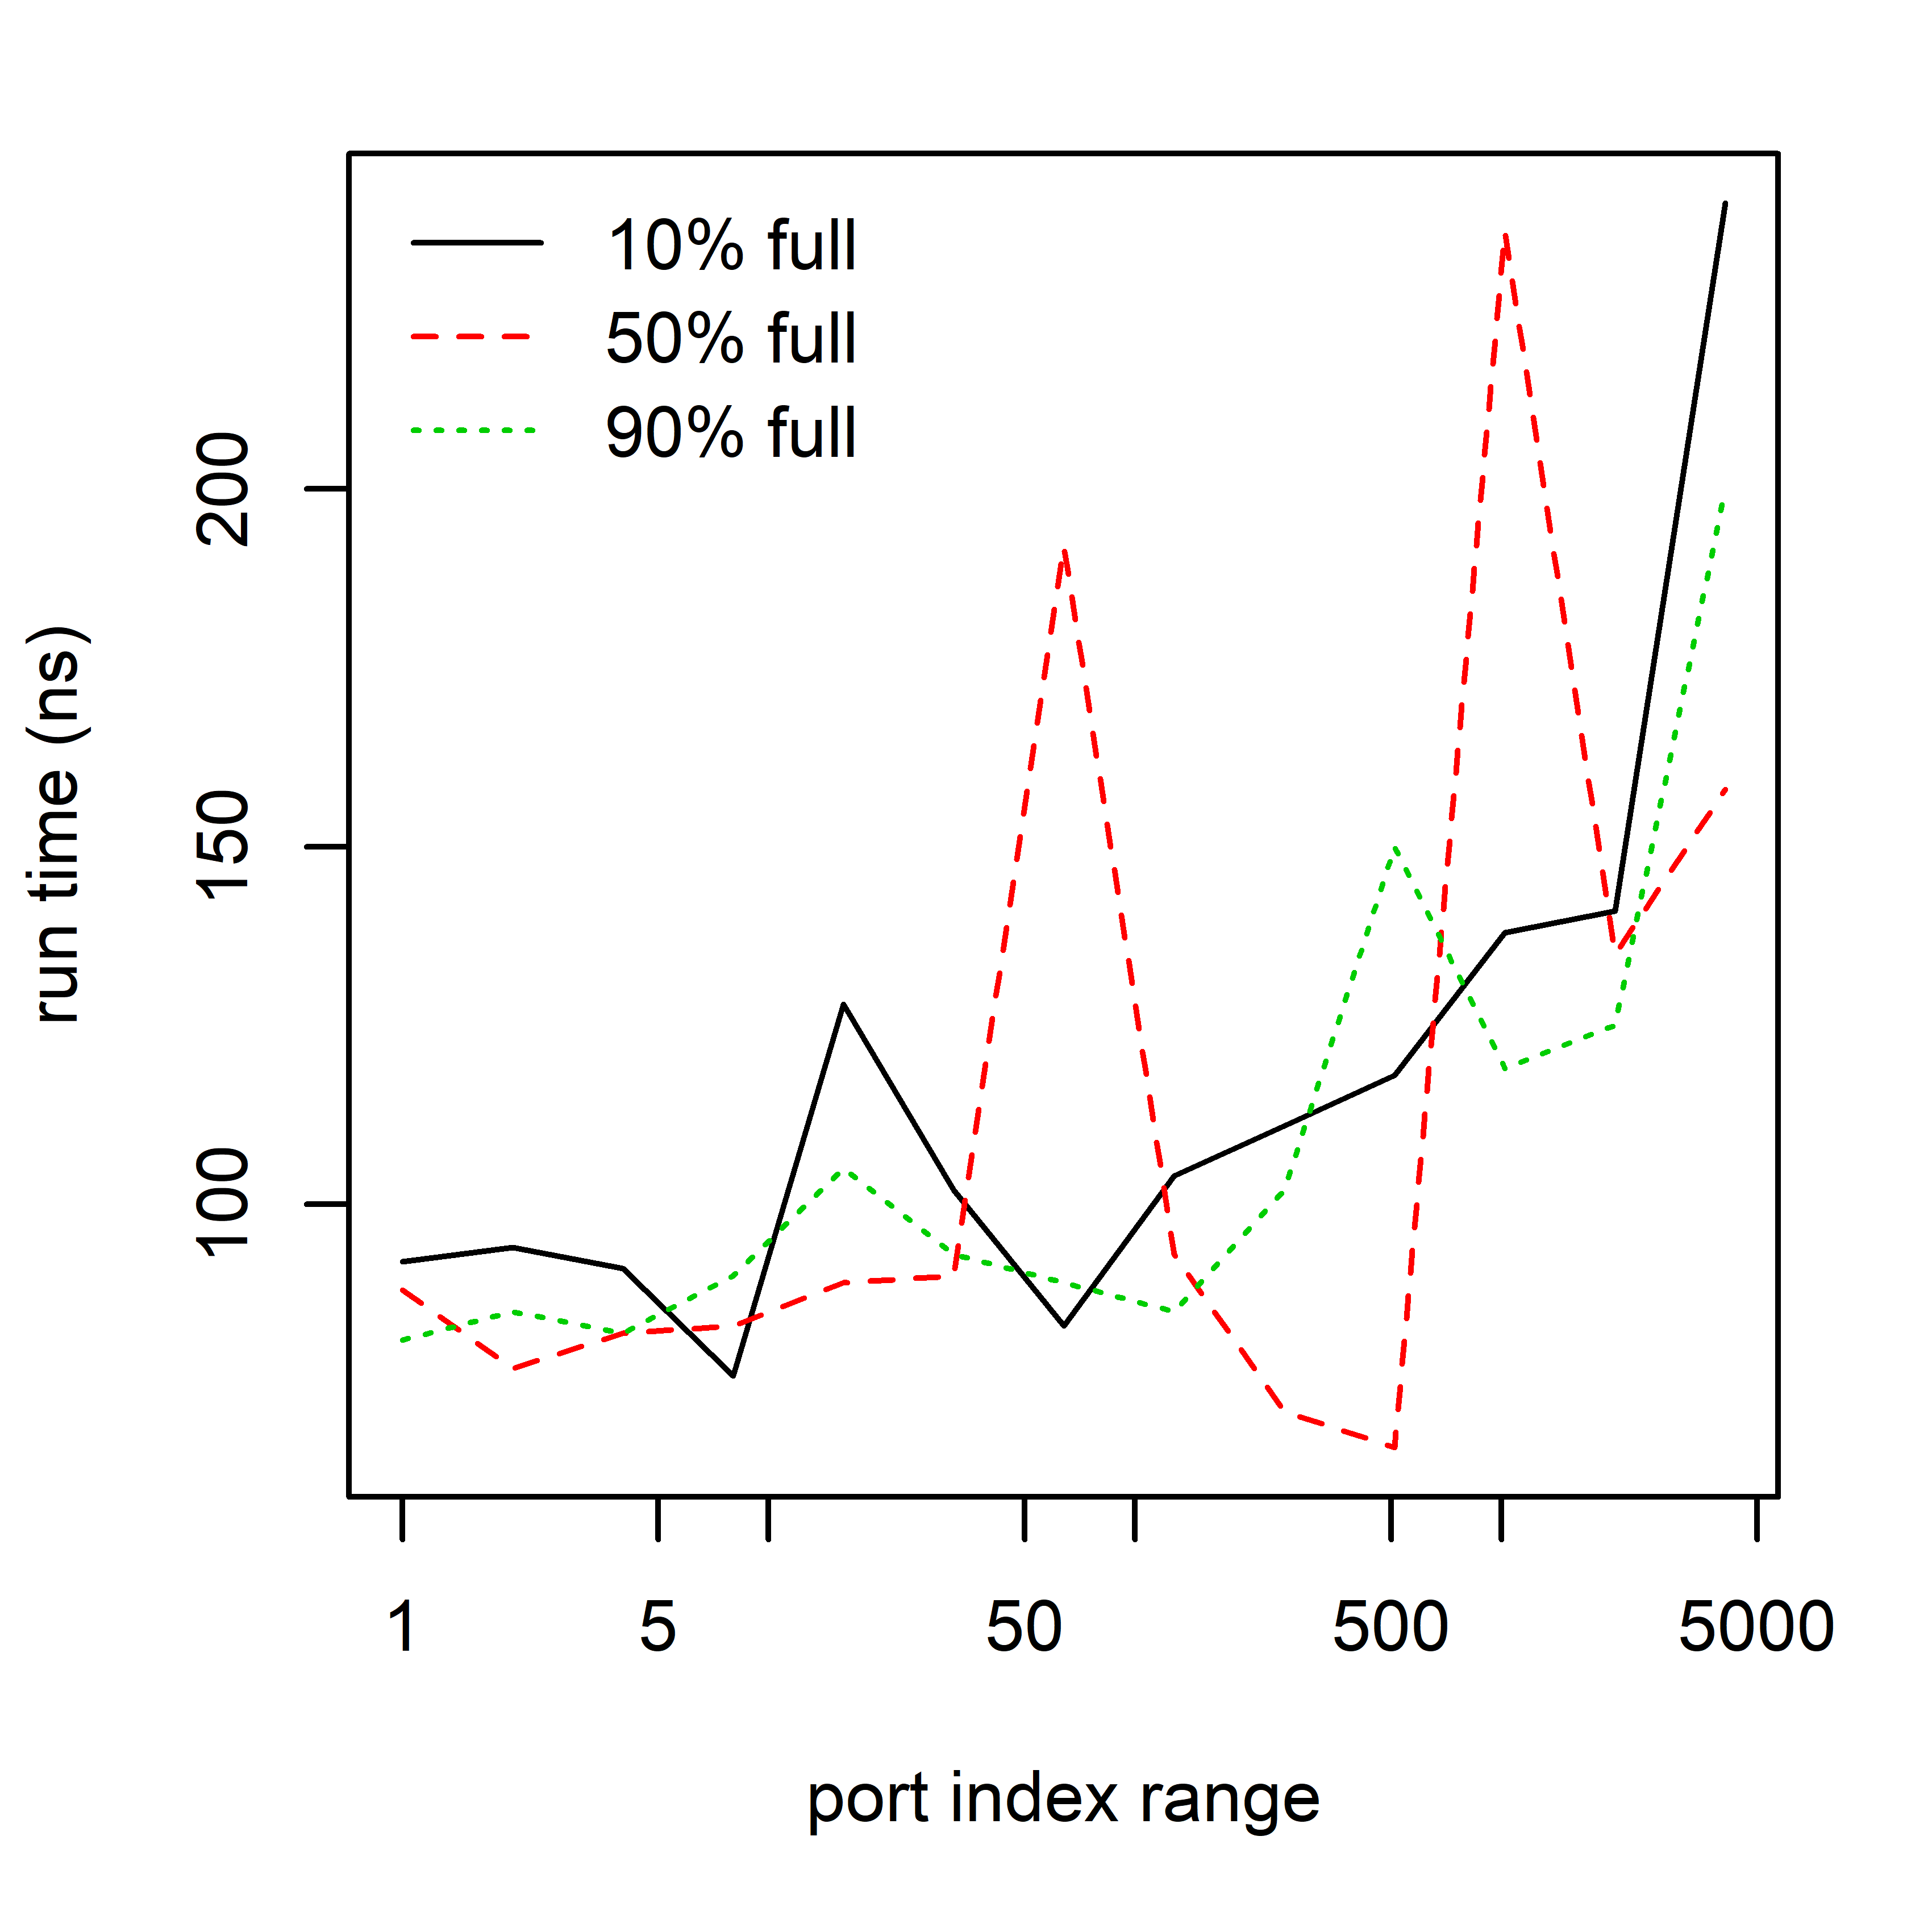
\includegraphics[width=\textwidth]{experiments/bits_0.png}
			\caption{}
			\label{fig:bits_0}
		\end{subfigure}%
		\begin{subfigure}[b]{0.63\textwidth}
			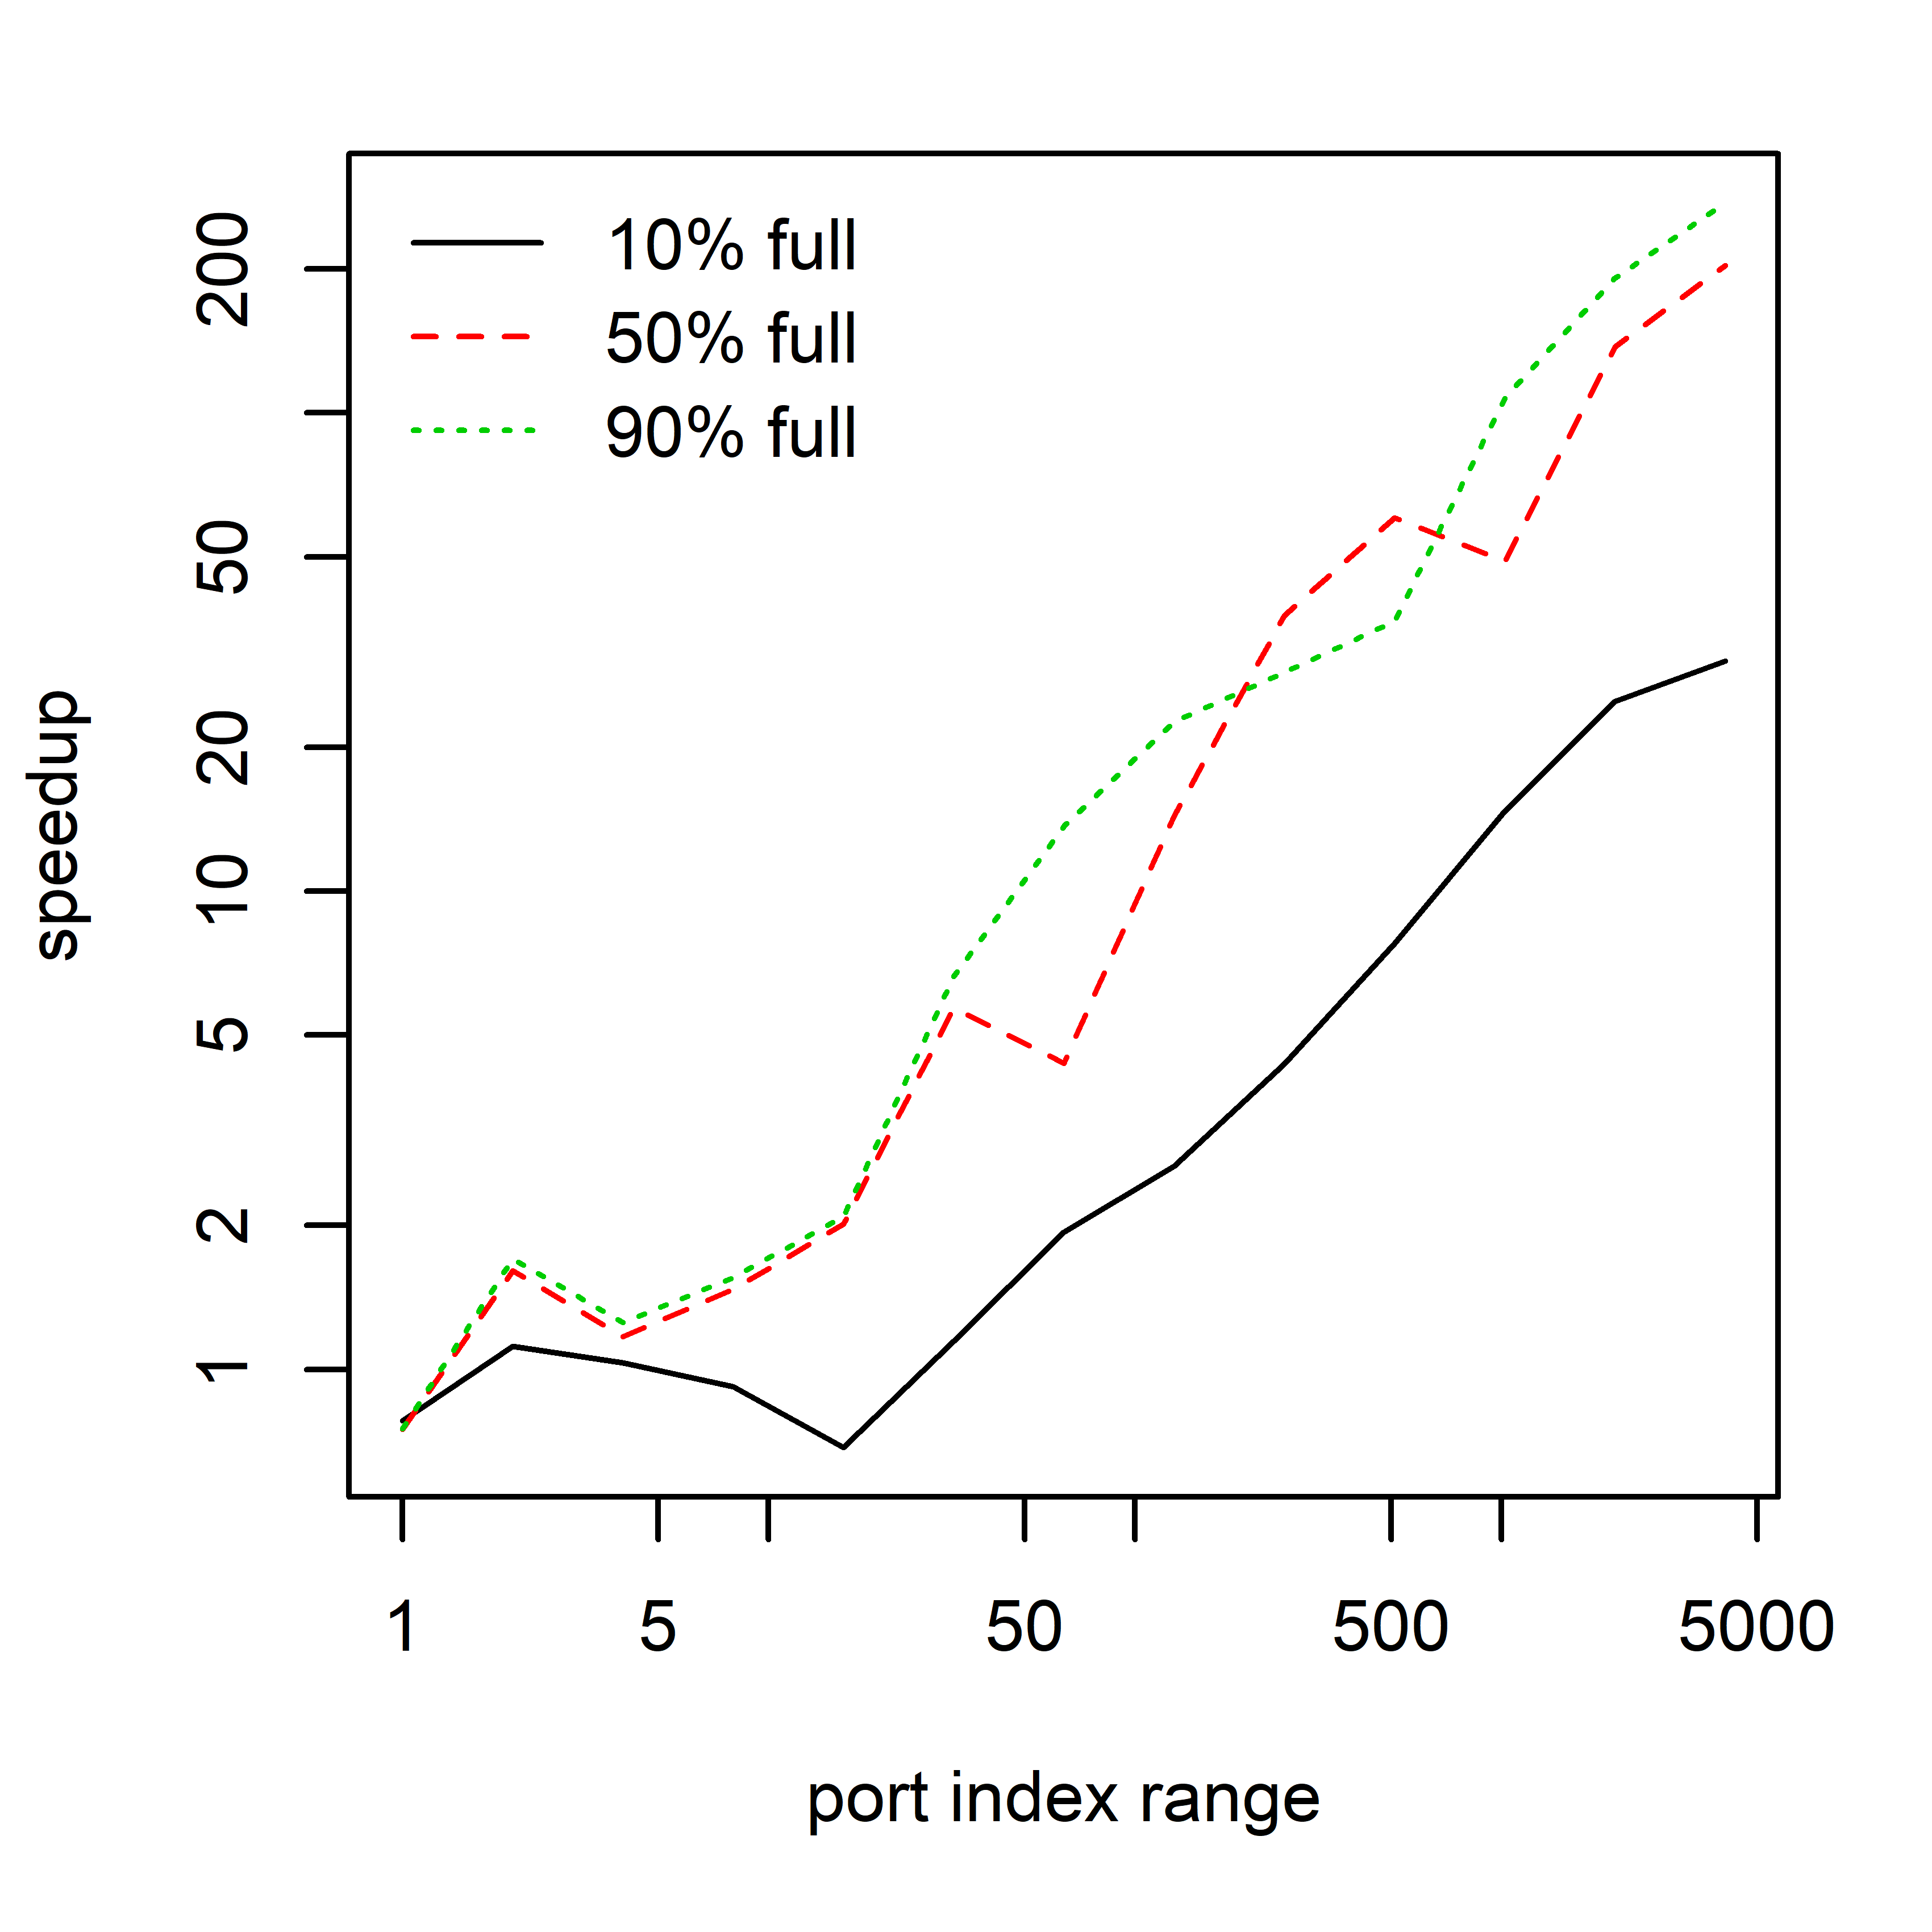
\includegraphics[width=\textwidth]{experiments/bits_1.png}
			\caption{}
			\label{fig:bits_1}
		\end{subfigure}%
	}
	\caption[Bit vector speedup over hashset.]{Run time of the \code{is\_subset} operation for bit vectors and canonical hash sets. This operation is used very frequently by the coordinator to determine whether a rule is satisfied. Figures show (a) run times for the bit vector in response to a changing maximal element, ie.\ number of ports, and (b) the speedup of the bit vector in comparison to the hash set. Note the logarithmic axes.}
	\label{fig:bits}
\end{figure}



The efficiency of the bit vector \textit{subset} operation is key to the speed of the coordinator. This is the first first three things evaluated for each and every rule, checking whether all involved ports are ready, and if all the relevant memory cells are full or empty. The bit-set capitalizes on how unusually often we need this operation. Figure~\ref{fig:bits} shows how bit vectors are very efficient at checking whether one is a subset of another. Here we see the time taken to evaluate the \textit{positive} case, representing the best-case scenario for our speedup. It is guaranteed to occur at least three times every time a rule fires. Figure~\ref{fig:bits_0} shows how low the cost of the operation stays, even when there are very many ports involved. Figure~\ref{fig:bits_1} shows how significant the speedup over the subset operation of canonical \code{HashSet} type. Admittedly, the majority of realistic Reo circuits are on the low-end with respect to number of ports; if nothing else, this is a result to encourage the development of more complex connectors. Observe that the cost of the operation is agnostic to the \textit{fullness} in the case of the bit-vector. This is not so for the hash set, for which a fuller hash set makes for a more expensive operation. 



\subsection{Overhead Outside the Critical Region}
After data exchanges are initiated by the coordinator, the protocol's lock is released. Time spent exchanging can therefore only impact the threads that play a part directly. Figure~\ref{fig:simo_copy} shows measurements of the \textit{siso} protocol, which synchronously distributes a putter's datum to a set of getters. First, we concentrate on the case where this datum implements the \code{Copy} trait, communicating to Reo-rs that it is safe to replicate elements of the ports' data type with bit-wise shallow copies. The experiment shows the mean time to finish one such interaction, varying in response to the size of the datum, and repeated for a different number of getters. As expected, runs with more getters took longer to complete, as the putter cannot return until everyone else is finished. The cost of the copy operations can also be seen to grow approximately linearly. Figure~\ref{fig:simo_copy_1} shows the runs normalized to that of the case with a single getter; here we observe that as the data gets larger, the overhead of the additional getters decreases in proportion to that of the single getter. The measurements for four and five getters are unexpectedly high compared to the rest. We are not able to fully explain this, and imagine it has something to do with these threads sharing resources with one another. Regardless, runs with these slower getters adhere to the prior observations, suggesting that whatever is influencing their performance is multiplying their overhead by a constant factor.
\begin{figure}
	\centering
	\makebox[\textwidth][c]{
		\begin{subfigure}[b]{0.63\textwidth}
			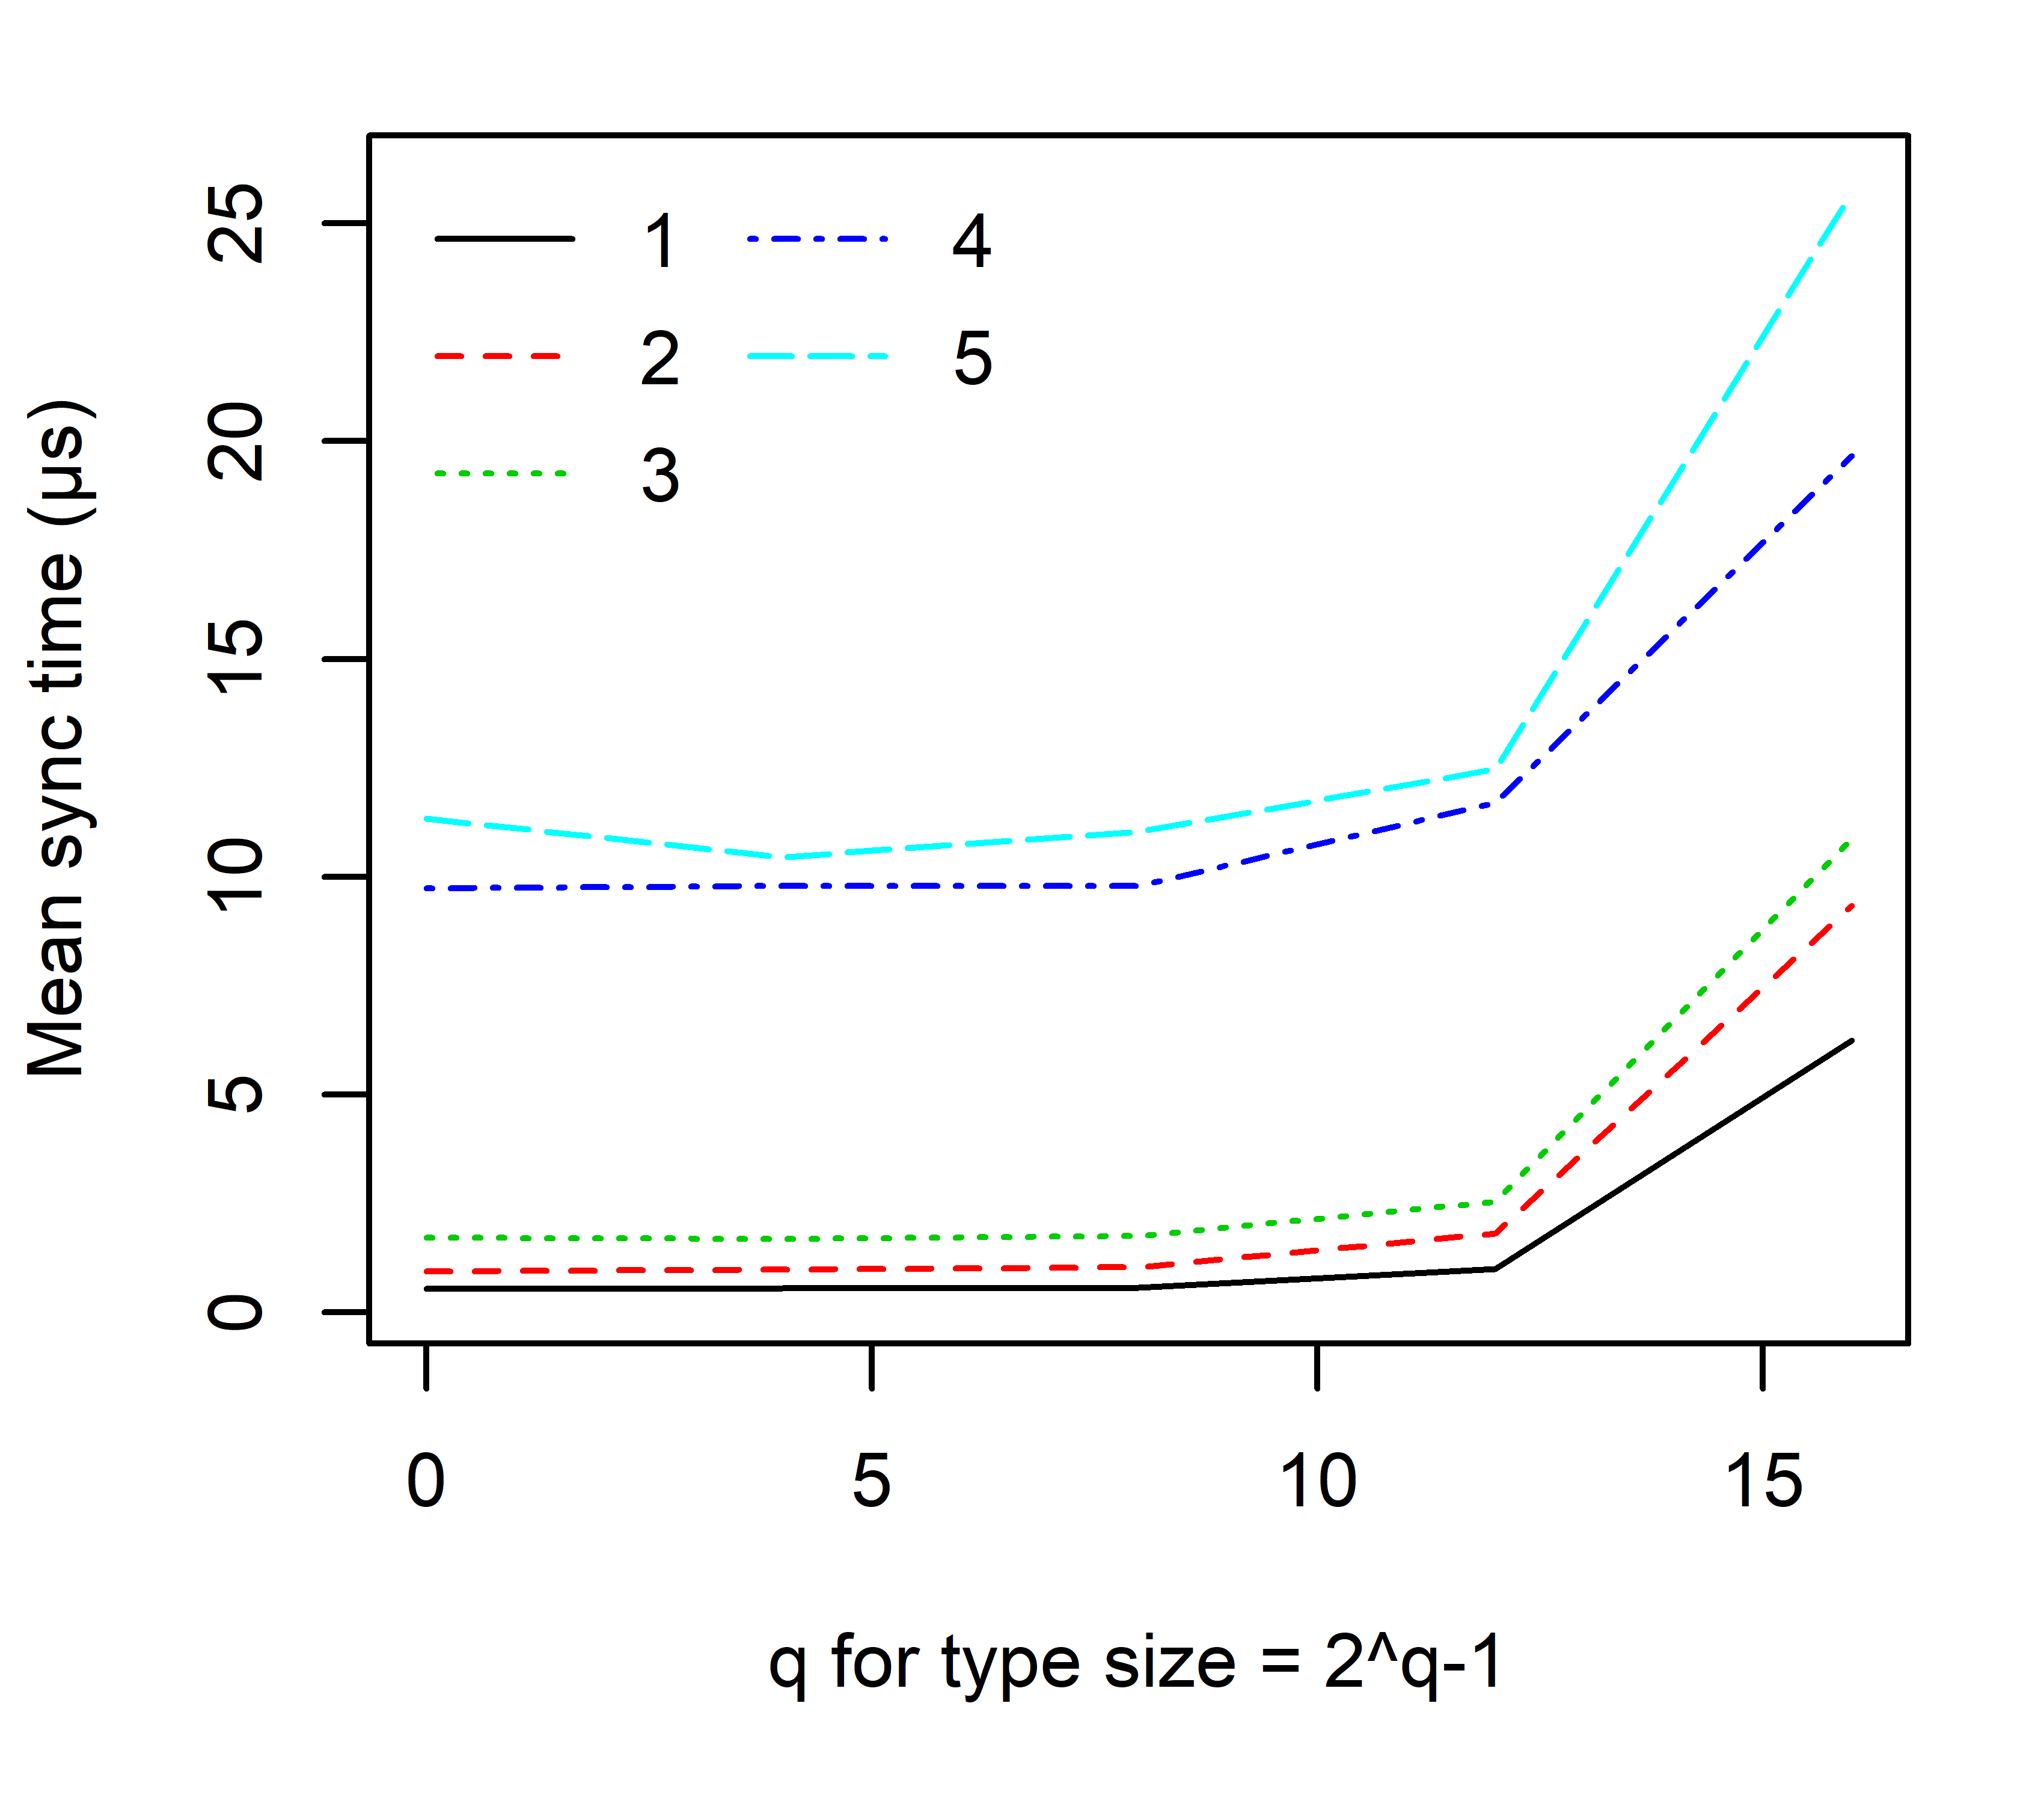
\includegraphics[width=\textwidth]{experiments/simo_copy_0.png}
			\caption{}
			\label{fig:simo_copy_0}
		\end{subfigure}%
		\begin{subfigure}[b]{0.63\textwidth}
			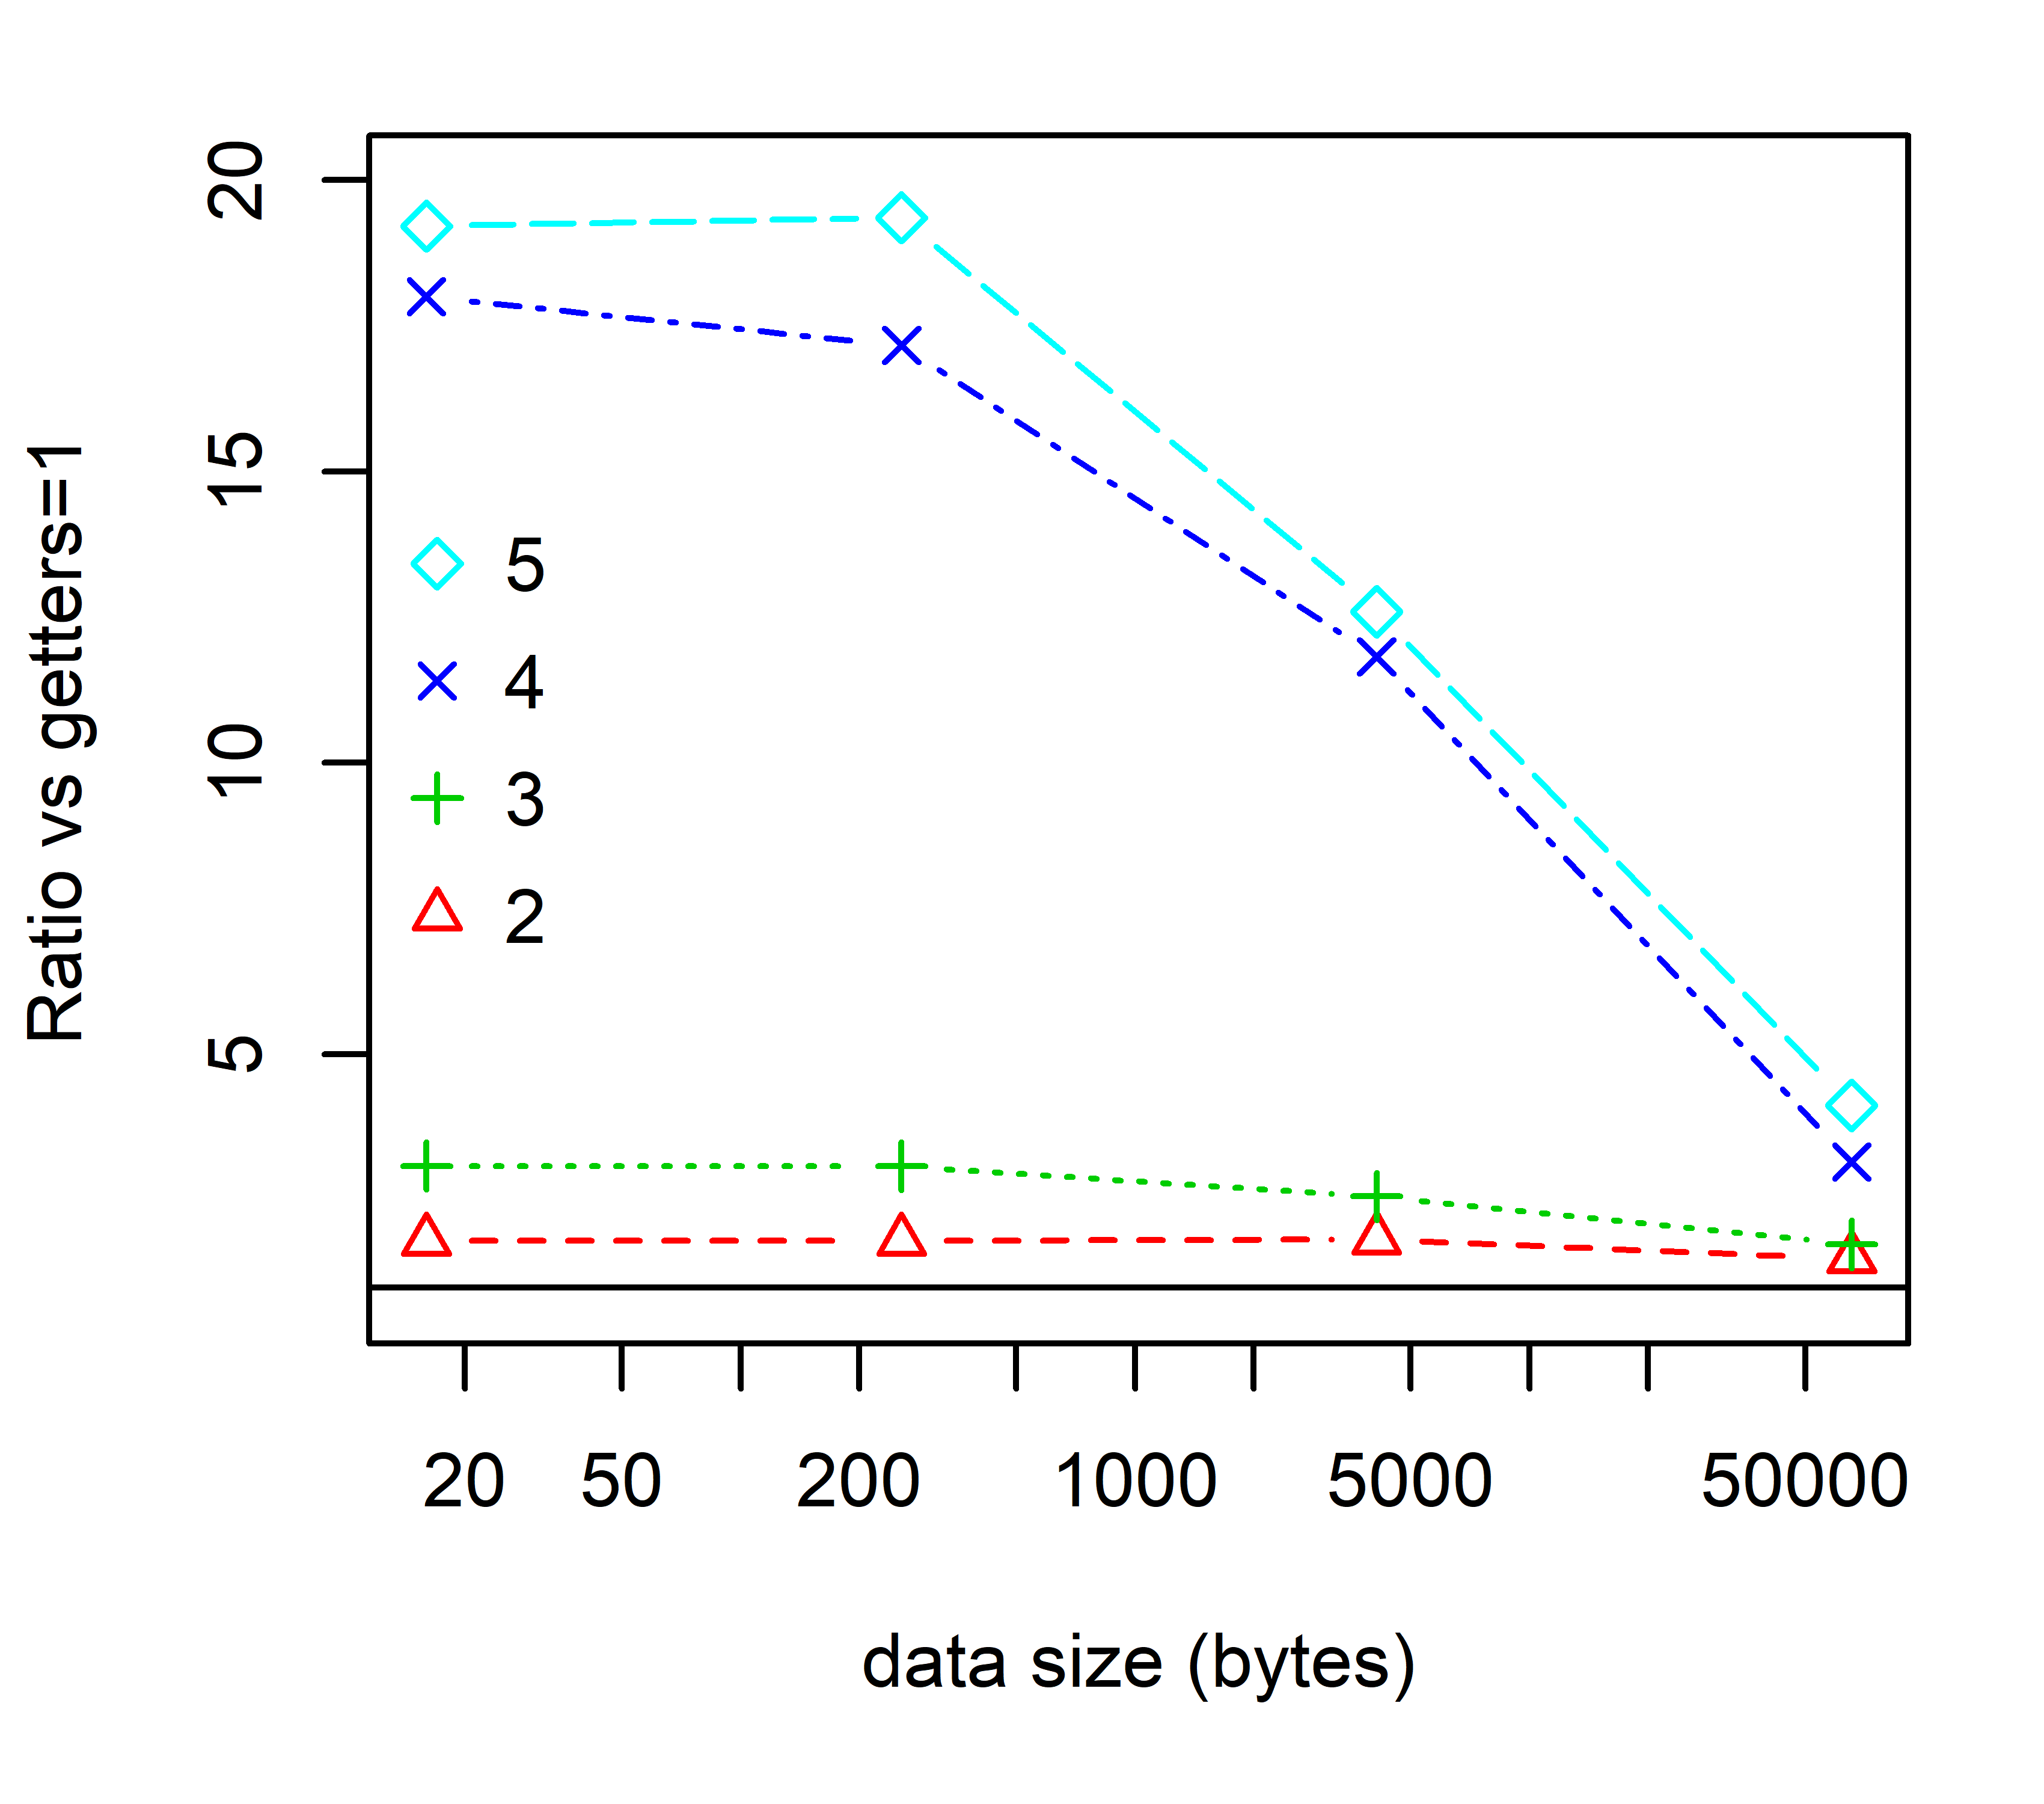
\includegraphics[width=\textwidth]{experiments/simo_copy_1.png}
			\caption{}
			\label{fig:simo_copy_1}
		\end{subfigure}%
	}
	\caption[Synchronization duration for SISO with copy-type data.]{Duration of a synchonization event from the perspective of a putter, putting to a set of getters. The data type implements \code{Copy}, allowing getters to copy the value bit-wise in parallel. Plots show five variants, corresponding to getter sets of sizes one through five, plotted in response to a data type with a changing size in memory.}
	\label{fig:simo_copy}
\end{figure}



The experiment with connector \textit{siso} is shown repeated in Figure~\ref{fig:clone_compete}. This time, the data type is not marked \code{Copy}. Section~\ref{sec:data_exchange} explains how the dissemination of these values to multiple getters are handled, as there are multiple requirements on the order of operations such that correctness can be guaranteed. In this context, Figure~\ref{fig:clone_compete_0} shows that the case of a single getter is exceptionally fast. This is to be expected, as even for non-copy data-types, all but one getter must clone; someone gets the putter's original. These results demonstrate the benefits of this optimization; it is worth noting that invoking a clone also incurs the overhead of an added \textit{virtual function call}.
In this experiment, the cost of \code{clone} was manipulated synthetically as before. As expected, beyond a threshold, the cost of the clone operation dominates, causing runtimes to converge, regardless of the number of getters.



\begin{figure}
	\centering
	\makebox[\textwidth][c]{
		\begin{subfigure}[b]{0.63\textwidth}
			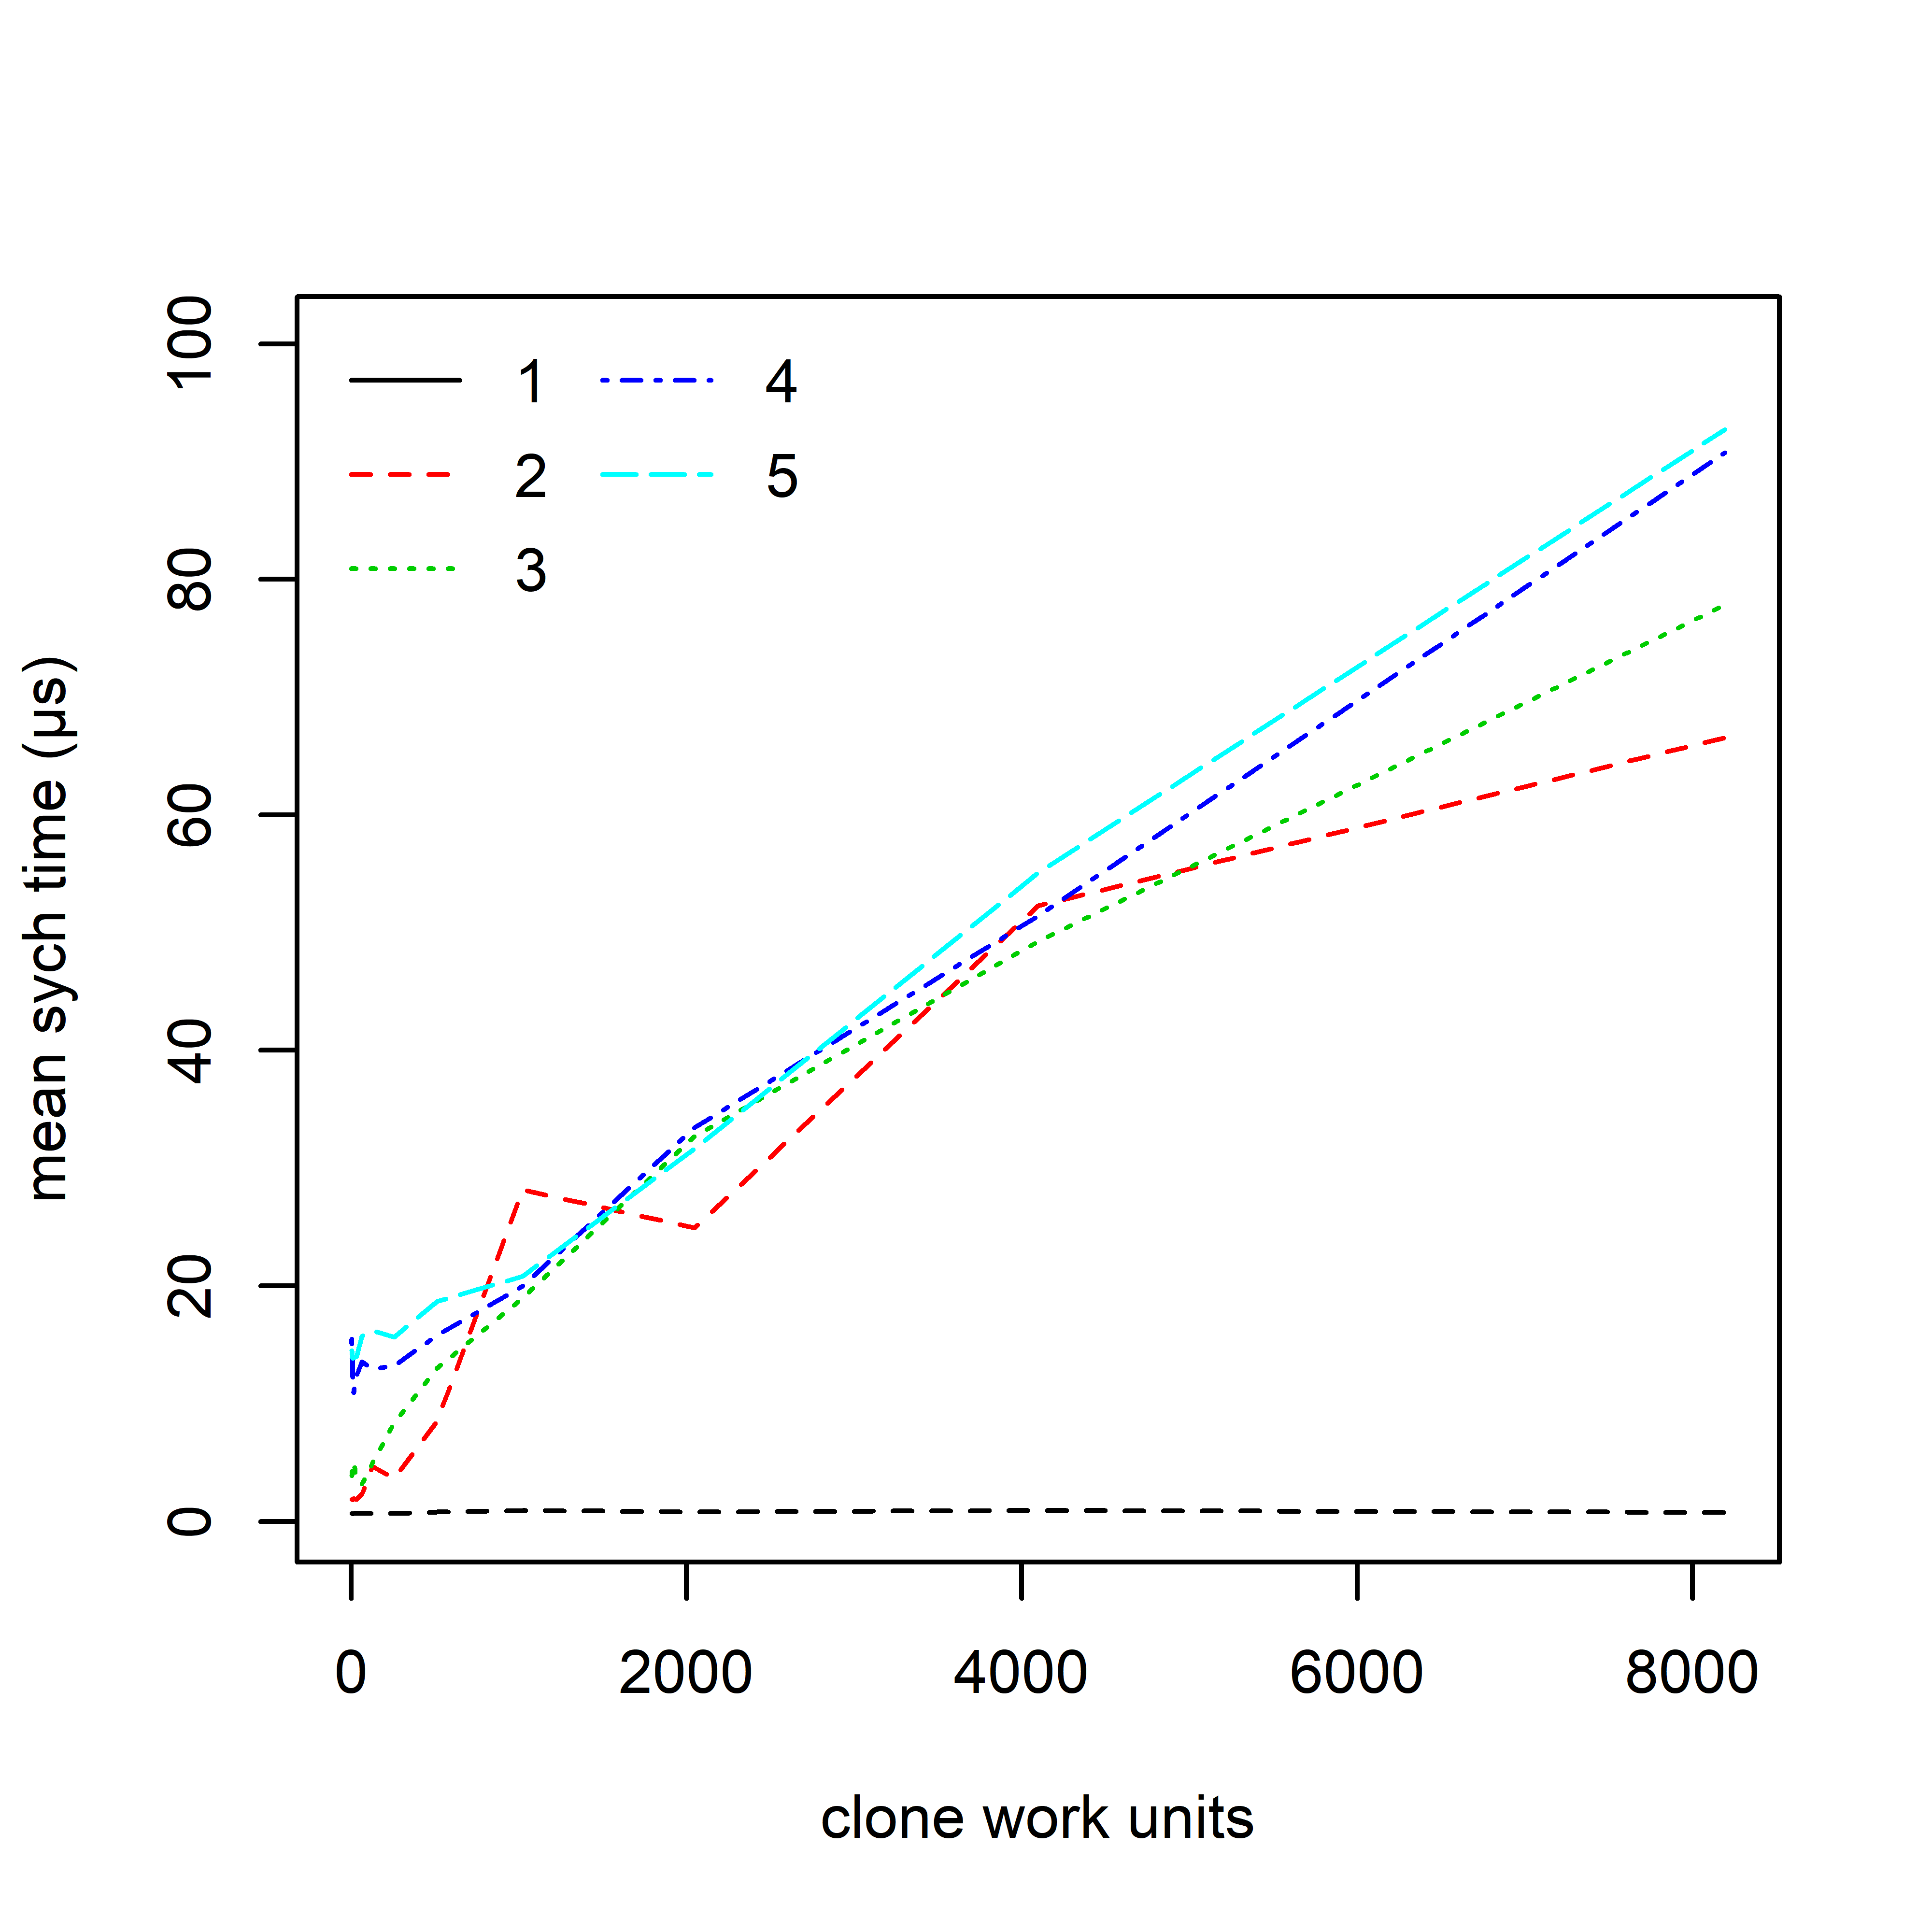
\includegraphics[width=\textwidth]{experiments/clone_compete_0.png}
			\caption{}
			\label{fig:clone_compete_0}
		\end{subfigure}%
		\begin{subfigure}[b]{0.63\textwidth}
			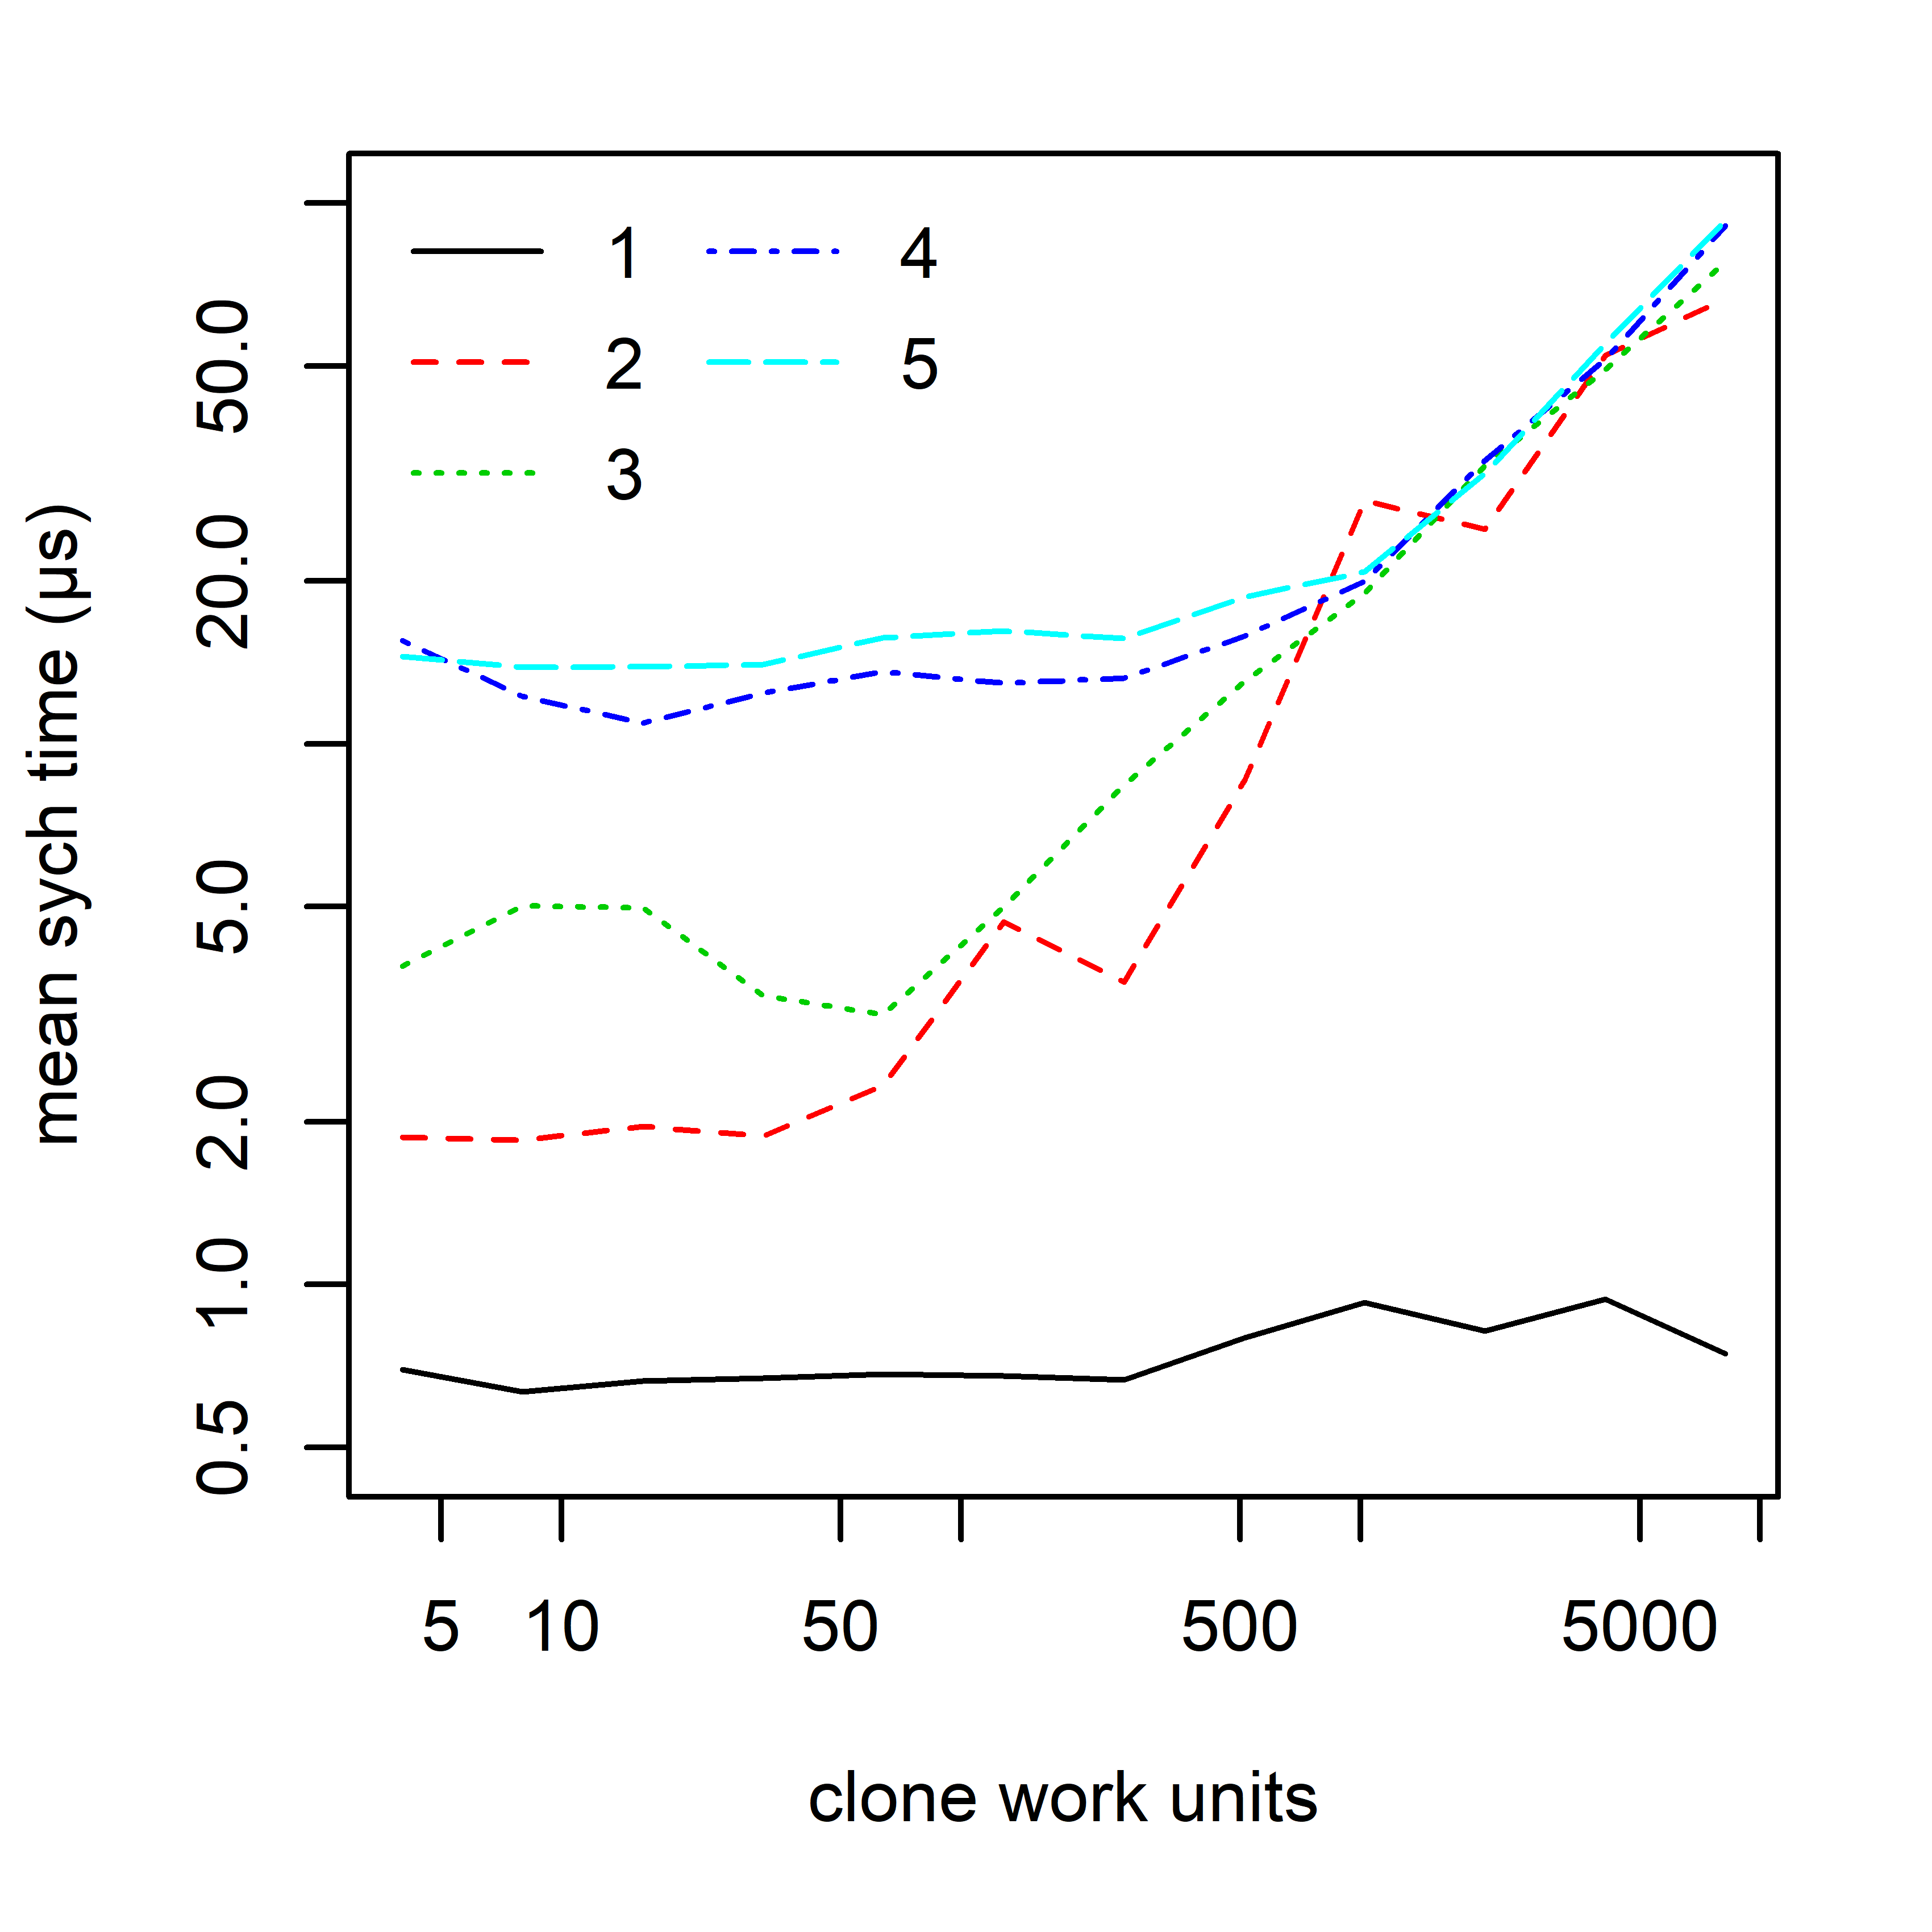
\includegraphics[width=\textwidth]{experiments/clone_compete_1.png}
			\caption{}
			\label{fig:clone_compete_1}
		\end{subfigure}%
	}
	\caption[Duration of interaction in siso connector with clonable data.]{Duration of an interaction in a \textit{siso} connector. Runs are distinguished by the number of getters per interaction with one putter, plotted over an increasingly expensive \code{clone} operation. Figure~(b) repeats the information of (a) to make the subtle differences more visible.}
	\label{fig:clone_compete}
\end{figure}


Figure~\ref{fig:clone_compete_2} omits the exceptional single-getter case to show the effects of competing cloners. Measurements for cheap clone operations differ in runtimes both as a result of increased contention on concurrency primitives, but also as a result of simply having a larger group of getters to wait for, giving more opportunities for stragglers to delay completion. 


\begin{figure}
	\centering
	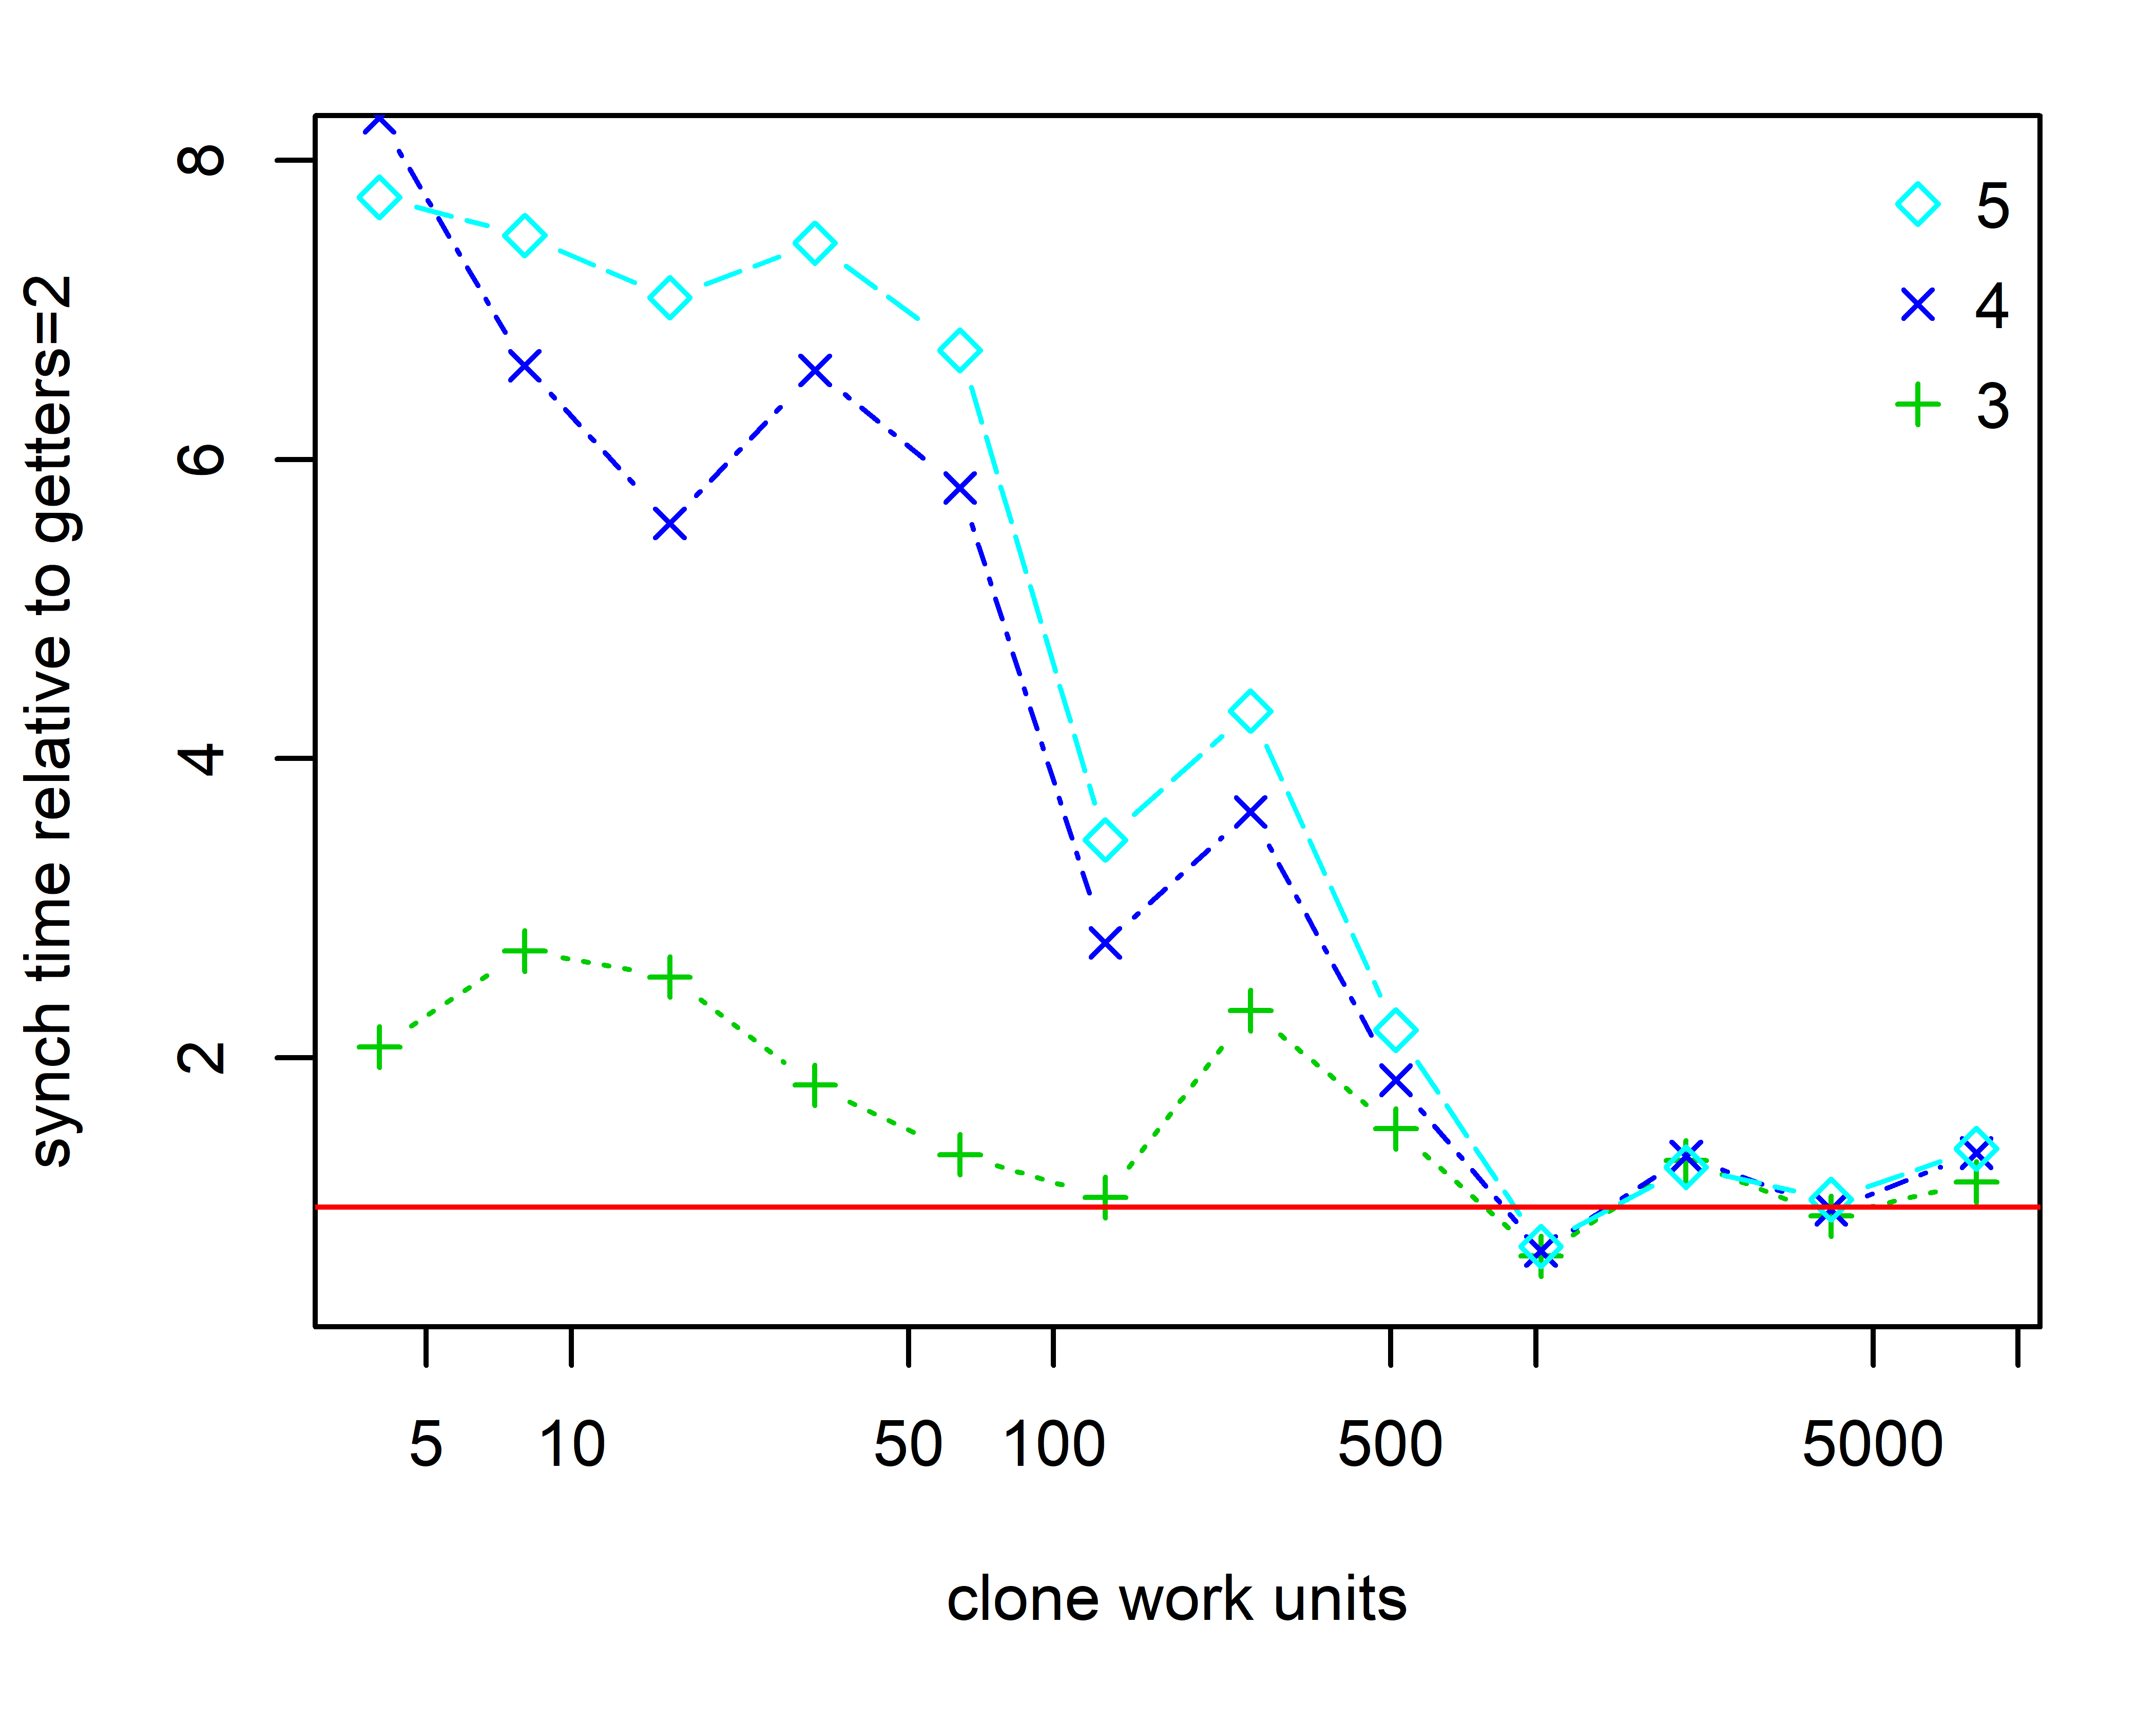
\includegraphics[width=0.80\textwidth]{experiments/clone_compete_2.png}
	\caption[Duration of interaction in siso connector with clonable data plotted relative to the speed of the 2-getter case.]{Measurements of all runs involving the \code{clone} operation from Figure~\ref{fig:clone_compete}, shown plotted relative to that of the case with 2-getters.}
	\label{fig:clone_compete_2}
\end{figure}


\part{Reflection}
\chapter{Discussion}
In this chapter, we reflect on the work and findings in Chapters~\ref{sec:imperative_form}--\ref{sec:benchmarking}. This includes a subjective assessment of the results of the project as a whole, and identification of promising directions for future work.

\label{sec:discussion}
\section{Future Work}
As with any project, there was insufficient time to investigate every topic we encountered. In this section, we highlight promising starting-points for future work related to Reo in general, or to our contributions in Chapters~\ref{sec:imperative_form}--\ref{sec:api}.

\subsection{Imperative Form Compiler}
Chapters~\ref{sec:imperative_form} and~\ref{sec:protocol_runtime} explain how the Reo-rs runtime makes use of a lightweight interpreter to bring life to our protocol objects at runtime according to the appropriate specification. This \textit{commandification} pattern has its advantages; namely, protocol behavior is alterable at runtime by manipulating the interpreted data. However, this flexibility does not come for free. The interpretation steps incur overhead both to the protocol construction procedure, and more importantly, to the work of \textit{port operations}. Fortunately, our \textit{imperative form} does not necessitate the use of an interpreter. Future work could investigate replacing the \code{build} procedure of Reo-rs with another compilation step such that the behavior is represented in native, directly-executable Rust. 

Futhermore, future work might investigate the use of custom \textit{domain specific languages} for compiling imperative form in a manner that it performs the same checking as in \code{build} \textit{statically}. the obvious means of doing this is to build a compiler from scratch. However, other options exist that can make better use of existing tools. For example, Rust's \textit{procedural macros} allow the programmer to define arbitrary transformations of Rust's \textit{abstract syntax trees} during compilation. Essentially, one is able to invoke arbitrary, pre-compiled Rust code \textit{inside} the user's Rust compiler itself. In this manner, one can embed the needed domain-specific language into the Rust compiler itself.

\subsection{Distributed Components}
This work focuses on coordination between threads in shared memory. This approach can already be applied in the context of distributed components by abstracting ports behind local ones. However, we are unable to distribute our protocol components, as they presuppose a single, monolithic shared state in our current scheme. One can get around this by fragmenting protocols into smaller ones, and distributing those smaller protocols across the system. However, this cannot currently be done in all cases, as this fragmentation does not preserve synchrony. 

Reo has a rich academic history in this distributed context. Future work might investigate how our contributions (eg.\ reference-passing optimizations, static governors, etc.) can be applied in distributed systems.


\subsection{Optimize Rule Branching}
\label{sec:future_branches}
Reo-rs is able to represent protocols whose rules contain \textit{branching}. Rule-based form has already shown us the correspondence between our RBA rules and propositional logic, where the formula corresponds to a protocol, with disjuncts as rules~\cite{dokter2018rule}. In the same way such terms can be manipulated until the formula is in \textit{disjunctive normal form}, so too are we able to remove branching from our rules by splitting them. For example, a rule with data constraint $(P_0=C_0\vee{}P_1=C_1)\wedge{}P_2=C_2$ can be converted into two rules with data constraints $P_0=C_0\wedge{}P_2=C_2$ and $P_0=C_0\wedge{}P_2=C_2$ respectively. Such transformations are not particularly meaningful to the outside observer; clearly they have  no influence on the protocol's semantics\footnote{Changing the granularity of rules can be semantically meaningful once it affects our ability to express interesting properties. For example, fine-grained rules can be desirable when the protocol is lifted to consider \textit{preference} between nondeterministic branching.}. However, they do have interesting implications on performance. It is easy to contrive of examples for both extreme ends of the spectrum for which this splitting is either beneficial or detrimental to the performance of the protocol object, as we are able to both introduce and eliminate redundant work by splitting rules. As an example of a rule \textit{not} worth splitting, consider one with very many \textit{instructions} $I$ before reaching a 3-way branch $a\vee{}b\vee{}c$ where the branch is not entirely nondeterministic (ie. there are cases for which $a$ cannot be chosen, etc.). Before splitting, $I$ is computed once, and then one of $\{a,b,c\}$ will occur. After splitting, three separate rules for $a$, $b$, and $c$ might be considered, each computing $I$ before the third fires successfully.

In our case, only the Reo compiler's internals perform manipulations on protocol rules, while Reo-rs restricts itself to the treatment of tautologies and contradictions. Future work might investigate more extensive manipulation of protocol rules to optimize rules by conditionally splitting them to remove branching.

\subsection{Runtime Governors}
Chapter~\ref{sec:api} explains how our design for static protocol governors is able to enforce protocol adherence at compile time. This approach is not always suitable, as it presupposes that we \textit{trust} the compilation process enforcing the governance. If the situation calls for a degree of separation between the compilation process and its use at runtime, this may no longer be a good choice. For example, consider the use of Reo to coordinate peers in a distributed system, where the behavior of a component originates from a remote source, traveling over the network.

Our static governors also have limitations on how finely they can distinguish the states of the protocol. In a perfect world, governors would use perfect models of the protocol's state. Section~\ref{sec:approximating_rba} gives an example of some practical reasons to approximate the protocol instead, resulting in a governor that attempts to strike a non-trivial balance between accuracy and simplicity of its local automaton. \textit{Dynamic} governors are given a far easier task, as they are able to make choices at runtime, when all the relevant information is available. Generally, these governors can therefore be more accurate. Future work might investigate how these two extremes of the spectrum compare, and to what extent it may be practical to use some facets of \textbf{both} to make an application more robust. There may be systems in which redundant checking is worth its cost to runtime performance.

\subsection{Further Runtime Optimization}
Section~\ref{sec:behavior_implementation} discusses various optimizations of Reo-rs's runtime performance applied in this work, chief of which is arguably the use of reference-passing inside the protocol's state as part of the implementation of rules such that it preserves Reo's value-passing semantics. Other optimization opportunities presented themselves during the project, but were not investigated thoroughly as they conflicted with our current goals, or were simply deemed less fruitful than other tasks. Future work might investigate these optimizations:

\begin{enumerate}
	\item Simplify rules in the context of a known \textit{priority ordering} on the rules to break nondeterminism. For example, given that rule $r_a$ has priority over rule $r_b$, the satisfaction of these rules must be checked in the same order; if $r_a$ fails, $r_b$ can be simplified such that is \textit{presumes} that $r_a$ did not hold. Such cases can occur frequently in practice, particularly when rules are split from branches, as dicussed in Section~\ref{sec:future_branches}. For example, consider rules  with data constraints $M_0=M_1$ and $M_0\neq{}M_1$; if these rules are prioritized in the order of their appearance here, the second rule can take the negation of the first's data constraint for granted, resulting in the second becoming trivial.
	
	\item Remove indirection inside Reo-rs when representing values smaller than the pointer-size, by `stuffing' the value inside the pointer field. This optimization has complex interactions with the \textit{memory storage} system described in Section~\ref{sec:memory_cells}, which uses pointers as keys to look up a value's reference count. Future work may investigate either (1) conditionally using stuffed pointers when it would not interact with the memory storage system, or (2) finding a way to make the memory storage system disambiguate these stuffed pointers
	
	
	\item More extensively pre-process the imperative form as its executable object is built (explained in Section~\ref{sec:translation_phase_2}). For example, instructions can be fragmented and re-organized such that the effects of a fired rule are unaltered, but rules are able to detect and recover from \textit{unsatisfied guards} and rolling back earlier.	
	
	\item Reduce the number of atomic operations used for the exchange of meta-information during data exchange (Section~\ref{sec:data_exchange}). Assuming realistic numbers of ports (ie. $2^{32}$) we are able to collapse several atomic operations into one, using modulo arithmetic. For example, we are able to increment two (logical) numbers using a single atomic counter by atomically adding $1 + 2^32$. In this fashion, the \textit{move} and \textit{countdown} variables may be unified to reduce lock contention.
	
	\item Some of the information currently exchanged between threads using atomics can be independently derived by reading the protocol's \textit{rules}. For example, getters can deduce their putter and whether they are permitted to move the datum this way, rather than being told by the coordinator explicitly. It is unclear whether this is an improvement, as these threads must spend extra time recovering this information, performing work redundant to that of the coordinator. 
\end{enumerate}
\subsection{Avoid Lock Re-Entry}
Section~\ref{sec:chosen_design} motivates the lack of a dedicated coordinator thread to back protocol objects at runtime. As a consequence, port-threads must share the responsibility of manipulating a shared protocol state in accordance with the protocol's movement through its configuration space. Protocols have non-trivial configuration spaces once they involve one or more memory cells in rules. To manipulate their contents safely, \textit{locks} are required around the shared `bookkeeping' structures that track these cells' states. Section~\ref{sec:data_exchange} explains how our design optimizes for the concurrency of rule-firings by moving the work of interacting with memory cells \textit{outside} of the critical reason. A consequence of this approach is the occasional need for threads to \textit{re-enter} the critical region to update the state of a memory cell. For example, the first lock event instigates the rule firing and updates state, but marks memory cell $M$ as `busy' to ensure it cannot be involved in a rule-firing until all \textit{data movements} outside the critical region have completed. Once done, some thread has the responsibility to mark $M$ as ready once again, necessitating a second lock event.

Future work might investigate more efficient mechanisms for achieving the same effect. As the mechanism is rather intricate, a vast space of possibilities exist. For example, one might investigate the effect of forgoing the second lock-event in favor of leaving a message for a later coordinator to handle. This could take the form of an efficient parallel-queue, highly optimized for the addition of new elements in parallel. More radical changes may also result in superior performance. Perhaps the locking can be avoided entirely if all the data structures representing the protocol's state become lock-free?

\subsection{Runtime Reconfiguration}
Chapter~\ref{sec:behavior_implementation} explains how Reo-rs uses a lightweight interpreter to implement protocol behavior at runtime, reading rules from a dense data structure. A result of this approach is the ability to alter a protocol object's behavior at runtime arbitrarily by manipulating the data representing its rules. Future work might investigate the introduction of a reconfiguration procedure to change the protocol without tearing the instance down or influencing the compute components in motion. The use of an interpreter trivializes the work of manipulating the rules themselves, but care must be taken to change the protocol object's \textit{meta-state} safely such that it results in a new protocol which is again internally consistent (eg.\ reconfiguring the structures used for primitive concurrency, message channels etc.).

\section{Conclusion}

The chosen design and implementation of a Rust code generator as part of the Reo compiler achieved satisfactory results. Despite usually being slower than a hand-written Rust program, our protocol objects were competitively performant in the case of non-trivial protocols. This is despite their data-oriented implementation, which has the added benefit of facilitating the \textit{reconfiguration} of a protocol's behavior at runtime. Exploiting this feature was out of the scope of this project, but provides an entrypoint for interesting future work.

By the nature of Reo, safety was always the primary concern of the behavior of our protocol objects at runtime. Still, this work also emphasized the importance of performance from its inception, motivating the choice of the Rust language in particular. The hope was to leverage its static \textit{ownership system} to achieve the reference-passing optimization employed by the Java backend, but free from its safety problems. However, the Rust compiler was not able to verify safety of interactions involving the transference of values between threads. Ultimately, our solution followed the Rust idiom of manually managing ownership within a minimal \textit{unsafe} scope, and wrapping it in an API that was safe once again. Rust's ownership and mutual-access semantics were invaluable for user-facing functionality for creating and destroying protocols and ports. Ultimately, we were able to provide an API that guarantees that a user cannot create ill-formed protocol or port objects, or experience system behavior that contradicts the specification of the protocol (unintentionally or otherwise) without intentionally circumventing Rust's safety semantics with unsafe code. Our design was able to avoid relying on specialized threads for protocol objects. Consequently, the user benefits from trivial protocol termination detection, and increased runtime performance for protocol objects repeatedly accessed by a single thread.

Rust's affine types were instrumental in our design of static governors, which allow a programmer to verify that their components do not threaten the liveness of the system at large almost entirely at compile-time. Our design demonstrates how an affine type system is able to communicate powerful correctness guarantees at compile-type across an API boundary. In our case, we are able to embed a complex requirement `the component does not perform a port-action that contradicts the specification of a stateful protocol' into terms the compiler can understand and enforce: preserve the affine semantics of variables. Our design allows the user to opt-into tasking their Rust compiler with performing this check themselves, effectively allowing them to extend the verification capabilities of their compiler with little more than a dependency. 


The complexity of the translation procedure from Reo to Rust
proved more complex than expected. Originally, the \textit{imperative form} intermediate representation was added out of necessity to curb the complexity of type-checking and various optimizations without bloating the Reo compiler itself with Rust-specifics. Unexpectedly, this introduction of this new form became integral to our protocol object's design, enabling us to extend its capabilities beyond what was originally intended. When compiling to Rust, the Reo compiler safely support more exotic Reo primitives such as \textit{filter} and \textit{transform}, which are able to perform \textit{tentative} computations as part of synchronous interactions. Imperative form also shows promise as an intermediary step for languages similar to Rust; it is conceivable that existing targets such as Java (or others not yet implemented) can leverage this representation to reduce the work of adding new language targets to the Reo compiler. 



\bibliographystyle{alpha}
\bibliography{references}

\end{document}